\documentclass[11pt,a4paper]{article}

\def\nyear {2025}
\def\nterm {Spring}
\def\nlecturer {Nir Lazarovich}
\def\ncourse {Algebraic Topology}

\makeatletter

% packages
\usepackage{amssymb,amsfonts,amsmath,calc,tikz,pgfplots,geometry,mathtools}
\usepackage{color}   % May be necessary if you want to color links
\usepackage[svgnames]{xcolor}
\usepackage[hidelinks]{hyperref}
\usepackage{forest}
\usepackage{commath} % ew
\usepackage{esvect} % \vv makes vectors
\usepackage{centernot} % for the comparison
\usepackage{esdiff}
\usepackage{esint}
\usepackage{amsthm}
\usepackage{fancyhdr}
\usepackage{bm}
\usepackage{witharrows}
\usepackage{bookmark}
\usepackage{tikz-cd}
\usepackage{quiver}
\usepackage{bbm}
\usepackage{textcomp}
\usepackage{float}
\usepackage{gensymb}
\usepackage{cleveref}
\usepackage{environ}
\usepackage{comment}
\usepackage{cancel}
\usepackage{xparse}

% Inevitable cs
\usepackage{listings}
\usepackage[]{algorithm2e}

% tikz libraries
\usetikzlibrary{positioning}
\usetikzlibrary{matrix}
\usetikzlibrary{arrows}
\usetikzlibrary{bending}
\usetikzlibrary{arrows.meta}
\usetikzlibrary{decorations.markings}
\usetikzlibrary{decorations.pathreplacing}
\usetikzlibrary{decorations.markings}
\usetikzlibrary{patterns}
\usetikzlibrary{backgrounds}

% Page style setup
\pagestyle{fancy}
\fancyhfoffset{0pt}
\renewcommand{\headwidth}{\textwidth}
\geometry{margin=1in}
\pgfplotsset{compat=1.18}
\setlength{\headheight}{14.6pt}
\addtolength{\topmargin}{-1.6pt}
\hypersetup{
    colorlinks=false,
    linktoc=section,
    linkcolor=black,
}

%% maketitle setup
\ifx \nauthor\undefined
  \def\nauthor{Yeheli Fomberg}
\else
\fi

\ifx \nemail\undefined
  \def\nemail{\href{mailto:yp@campus.technion.ac.il}
  {\texttt{<yp@campus.technion.ac.il>}}}
\else
\fi

\ifx \ncoursehead \undefined
  \def\ncoursehead{\ncourse}
\fi

\lhead{\emph{\nouppercase{\leftmark}}}
\ifx \nextra \undefined
  \rhead{
    \ifnum\thepage=1
    \else
      \ncoursehead
    \fi}
\else
  \rhead{
    \ifnum\thepage=1
    \else
      \ncoursehead \ (\nextra)
    \fi}
\fi

\def\notes{notes}
\def\problems{problems}

\ifx \ntype \undefined
  \def\ntype{notes}
\else
\fi

\ifx \ntype \notes
  \let\@real@maketitle\maketitle
  \renewcommand{\maketitle}{\@real@maketitle\begin{center}
  \begin{minipage}[c]{0.9\textwidth}\centering\footnotesize
  These notes are not endorsed by the lecturers.
  I have revised them outside lectures to incorporate supplementary
  explanations, clarifications, and material for fun.
  While I have strived for accuracy, any errors or misinterpretations 
  are most likely mine.
  \end{minipage}\end{center}}
\else
  \ifx \ntype \problems
    \let\@real@maketitle\maketitle
    \renewcommand{\maketitle}{\@real@maketitle\begin{center}
    \begin{minipage}[c]{0.9\textwidth}\centering\footnotesize
    These problems are mostly based on the problem sets I was given
    when taking the course.
    
    While I have strived for accuracy and completeness,
    some of the problems would not have been here without the help of
    friends.
    \end{minipage}\end{center}}
  \else
  \fi
\fi


% theorem environments
\theoremstyle{definition}
\newtheorem{definition}{Definition}[section]
\newtheorem{remark}{Remark}[section]
\newtheorem{example}{Example}[section]
\newtheorem{exercise}{Exercise}[section]
\newtheorem{paradox}{Paradox}[section]
\newtheorem{entry}{Entry}[section]
\newtheorem*{solution}{Solution}
\newtheorem*{question}{Question}
\newtheorem*{answer}{Answer}
\newtheorem*{problem}{Problem}
\theoremstyle{plain}
\newtheorem{theorem}{Theorem}[section]
\newtheorem{proposition}[theorem]{Proposition}
\newtheorem{lemma}[theorem]{Lemma}
\newtheorem{corollary}[theorem]{Corollary}
\newenvironment{proofof}[1]{%
    \renewcommand{\proofname}{Proof of #1}%
    \begin{proof}
}{%
    \end{proof}
}
% tikz customization
\pgfarrowsdeclarecombine{twolatex'}{twolatex'}{latex'}{latex'}{latex'}{latex'}
\tikzset{->/.style = {decoration={markings,
                                  mark=at position 0.999
                                  with {\arrow[scale=2]{latex'}}},
                      postaction={decorate}}}
\tikzset{<-/.style = {decoration={markings,
                                  mark=at position 0.001 with {\arrowreversed[scale=2]{latex'}}},
                      postaction={decorate}}}
\tikzset{-->/.style = {decoration={markings,
                                  mark=at position 0.999
                                  with {\arrow[scale=2]{latex'[sep=0pt -2.5]}}},
                      postaction={decorate}}}
\tikzset{<--/.style = {decoration={markings,
                                  mark=at position 0.001
                                  with {\arrowreversed[scale=2]{latex'[sep=0pt -2.5]}}},
                      postaction={decorate}}}
\tikzset{<->/.style = {decoration={markings,
                                  mark=at position 0.001 with {\arrowreversed[scale=2]{latex'}},
                                  mark=at position 0.999 with {\arrow[scale=2]{latex'}},},
                      postaction={decorate}}}
\tikzset{->-/.style = {decoration={markings,
    mark=at position 0.50+0.225/#1 with {\arrow[scale=2]{latex'}}},
                      postaction={decorate}}}
\tikzset{-<-/.style = {decoration={markings,
                                   mark=at position 0.50-0.225/#1 with {\arrowreversed[scale=2]{latex'}}},
                       postaction={decorate}}}
\tikzset{->>/.style = {decoration={markings,
                                  mark=at position 1 with {\arrow[scale=2]{latex'}}},
                      postaction={decorate}}}
\tikzset{<<-/.style = {decoration={markings,
                                  mark=at position 0 with {\arrowreversed[scale=2]{twolatex'}}},
                      postaction={decorate}}}
\tikzset{<<->>/.style = {decoration={markings,
                                   mark=at position 0 with {\arrowreversed[scale=2]{twolatex'}},
                                   mark=at position 1 with {\arrow[scale=2]{twolatex'}}},
                       postaction={decorate}}}
\tikzset{->>-/.style = {decoration={markings,
                                   mark=at position 0.50+0.450/#1 with {\arrow[scale=2]{twolatex'}}},
                       postaction={decorate}}}
\tikzset{-<<-/.style = {decoration={markings,
                                   mark=at position 0.50-0.450/#1 with {\arrowreversed[scale=2]{twolatex'}}},
                       postaction={decorate}}}

\pgfarrowsdeclare{biggertip}{biggertip}{%
  \setlength{\arrowsize}{1pt}
  \addtolength{\arrowsize}{.1\pgflinewidth}
  \pgfarrowsrightextend{0}
  \pgfarrowsleftextend{-5\arrowsize}
}{%
  \setlength{\arrowsize}{1pt}
  \addtolength{\arrowsize}{.1\pgflinewidth}
  \pgfpathmoveto{\pgfpoint{-5\arrowsize}{4\arrowsize}}
  \pgfpathlineto{\pgfpointorigin}
  \pgfpathlineto{\pgfpoint{-5\arrowsize}{-4\arrowsize}}
  \pgfusepathqstroke
}
\tikzset{
	EdgeStyle/.style = {>=biggertip}
}

\tikzset{circ/.style = {fill, circle, inner sep = 0, minimum size = 3}}
\tikzset{scirc/.style = {fill, circle, inner sep = 0, minimum size = 1.5}}
\tikzset{mstate/.style={circle, draw, black, text=black, minimum width=0.7cm}}

\tikzset{eqpic/.style={baseline={([yshift=-.5ex]current bounding box.center)}}}

\definecolor{mblue}{rgb}{0.2, 0.3, 0.8}
\definecolor{morange}{rgb}{1, 0.5, 0}
\definecolor{mgreen}{rgb}{0, 0.4, 0.2}
\definecolor{mred}{rgb}{0.5, 0, 0}

% topology
\DeclareMathOperator{\dfr}{dfr} % deformation retract
\newcommand{\Cells}{\text{Cells}}
\newcommand{\RP}{\mathbb{RP}}
\newcommand{\CP}{\mathbb{CP}}

% order theory
\newcommand{\join}{\vee}
\newcommand{\meet}{\wedge}

% algebraic geometry
\DeclareMathOperator{\Rad}{Rad} % Radical of modules
\DeclareMathOperator{\Spec}{Spec}
% \renewcommand{\div}{\mathrm{div}} % divisors
\DeclareMathOperator{\Mer}{Mer} % Meromorphic functions
\DeclareMathOperator{\Exc}{Exc} % Exceptional divisor
\DeclareMathOperator{\Td}{Td} % Todd classes

% algebra

\DeclareMathOperator{\trdeg}{tr.deg.}
\DeclareMathOperator{\odd}{odd}
\DeclareMathOperator{\even}{even}
\DeclareMathOperator{\lcm}{lcm}
\DeclareMathOperator{\ord}{ord}
\DeclareMathOperator{\codim}{codim}
\DeclareMathOperator{\Ann}{Ann}
\DeclareMathOperator{\Ext}{Ext}
\DeclareMathOperator{\Sym}{Sym}
\DeclareMathOperator{\Out}{Out}
\DeclareMathOperator{\Aut}{Aut}
\DeclareMathOperator{\End}{End}
\DeclareMathOperator{\Inn}{Inn}
\DeclareMathOperator{\Mat}{Mat}
\DeclareMathOperator{\Fix}{Fix}
\DeclareMathOperator{\std}{std}
\DeclareMathOperator{\sgn}{sgn}
\DeclareMathOperator{\adj}{adj}
\DeclareMathOperator{\id}{id}
\DeclareMathOperator{\op}{op}
\DeclareMathOperator{\tr}{tr}
\DeclareMathOperator{\diag}{diag}
\DeclareMathOperator{\rank}{rank}
\DeclareMathOperator{\rk}{rk}
\DeclareMathOperator{\coker}{coker}
\DeclareMathOperator{\Mult}{Mult} % multiplier algebra
\DeclareMathOperator{\Frac}{Frac} % fraction field
\DeclareMathOperator{\Rat}{Rat}
\DeclareMathOperator{\Gal}{Gal}
\newcommand{\ioplus}{\overset{\text{int}}{\oplus}} % interior direct sum
\newcommand{\GG}{\mathcal G} % Galois correspondence
\newcommand{\FF}{\mathcal F} % Galois correspondence
\newcommand{\cupp}{\smile} % cup product
\newcommand{\capp}{\frown} % cap product
\newcommand{\actson}{\curvearrowright}
\newcommand{\bra}{\left\langle}
\newcommand{\ket}{\right\rangle}
\newcommand{\idealin}{\triangleleft\,}
\newcommand{\normalin}{\triangleleft\,}
\newcommand{\ip}[2]{\left\langle #1, #2 \right\rangle}
\newcommand{\bigslant}[2]
{{\raisebox{.2em}{$#1$}\left/\raisebox{-.2em}{$#2$}\right.}}
\newcommand{\properideal}{%
  \mathrel{\ooalign{$\lneq$\cr\raise.22ex\hbox{$\lhd$}\cr}}}

% categories
\newcommand{\cat}[1]{\mathbf{#1}}
\newcommand{\Ch}{\cat{Ch}} % Chain complexes   
\newcommand{\Set}{\cat{Set}}
\newcommand{\Grp}{\cat{Grp}}
\newcommand{\Ab}{\cat{Ab}}
\newcommand{\Ring}{\cat{Ring}}
\newcommand{\CRing}{\cat{CRing}}
\newcommand{\Top}{\cat{Top}}
\newcommand{\Vect}{\cat{Vect}}
\newcommand{\cmod}{\cat{mod}}

%% matrix groups
\newcommand{\GL}{\mathrm{GL}}
\newcommand{\Or}{\mathrm{O}}
\newcommand{\PGL}{\mathrm{PGL}}
\newcommand{\PSL}{\mathrm{PSL}}
\newcommand{\PSO}{\mathrm{PSO}}
\newcommand{\PSU}{\mathrm{PSU}}
\newcommand{\SL}{\mathrm{SL}}
\newcommand{\msl}{\mathrm{sl}}
\newcommand{\SO}{\mathrm{SO}}
\newcommand{\Spin}{\mathrm{Spin}}
\newcommand{\Sp}{\mathrm{Sp}}
\newcommand{\SU}{\mathrm{SU}}
\newcommand{\U}{\mathrm{U}}
\let\char\relax
\newcommand{\char}{\text{char}}

% analysis
\renewcommand{\Re}{\mathrm{Re}}
\renewcommand{\Im}{\mathrm{Im}}
\NewDocumentCommand{\dx}{o}{
  \IfNoValueTF{#1}
    {\dif x}                  % if no optional argument
    {\dif^{#1} \!x}         % if optional argument
}
\NewDocumentCommand{\dy}{o}{
  \IfNoValueTF{#1}
    {\dif y}                  % if no optional argument
    {\dif^{#1} \!y}         % if optional argument
}
\newcommand{\dt}{\dif t}
\newcommand{\du}{\dif u}
\newcommand{\dv}{\dif v}
\newcommand{\dz}{\dif z}
\newcommand{\ds}{\dif s}
\newcommand{\dw}{\dif w}
\newcommand{\dr}{\dif r}
\newcommand{\dm}{\dif m}
\newcommand{\df}{\dif f}
\newcommand{\dV}{\dif V}
\newcommand{\dS}{\dif S}
\newcommand{\dA}{\dif \mathrm{A}}
\newcommand{\dmu}{\dif \mu}
\newcommand{\dnu}{\dif \nu}
\newcommand{\dtheta}{\dif \theta}
\newcommand{\domega}{\dif \omega}
\newcommand{\dsigma}{\dif \sigma}
\newcommand{\dtau}{\dif \tau}
\newcommand{\dvarphi}{\dif \varphi}
\renewcommand{\dif}{\mathrm{d}}
\renewcommand{\Dif}{\mathrm{D}}
\renewcommand{\triangle}{\Delta}
\newcommand{\ptriangle}{\partial \triangle}
\DeclareMathOperator{\im}{im}
\DeclareMathOperator{\cis}{cis}
\DeclareMathOperator{\rot}{rot}
\DeclareMathOperator{\vspan}{span}
\DeclareMathOperator{\grad}{grad}
\DeclareMathOperator{\curl}{curl}
\DeclareMathOperator{\esssup}{esssup}
\newcommand{\hodge}{{\mathnormal{\star}}}
\DeclareMathOperator{\range}{range}
\DeclareMathOperator{\Hom}{Hom}
\DeclareMathOperator{\Int}{Int}
\DeclareMathOperator{\Conv}{Conv} % convex hull
\newcommand{\ind}{\mathbbm{1}}
\DeclareMathOperator{\Res}{Res}
\DeclareMathOperator{\graph}{graph}
\DeclareMathOperator{\diam}{diam}
\DeclareMathOperator{\supp}{supp}
\DeclareMathOperator{\Vol}{Vol} % Volume
\DeclareMathOperator{\Area}{Area} % Area
\DeclareMathOperator{\area}{area}
\DeclareMathOperator{\Ind}{Ind} % Index
\newcommand{\length}{\mathrm{length}}

% logic
\DeclareMathOperator{\MOD}{MOD}
\DeclareMathOperator{\Theory}{Theory}
\newcommand{\notimplies}{%
  \mathrel{{\ooalign{\hidewidth$\not\phantom{=}$\hidewidth\cr$\implies$}}}}

% nice
\newcommand{\half}{\frac{1}{2}}
\newcommand{\pair}{\del}
\newcommand{\taking}[1]{\xrightarrow{#1}}
\newcommand{\otaking}[1]{\xleftarrow{#1}}
\newcommand{\inv}{^{-1}}
\newcommand{\ot}{\leftarrow}
\newcommand{\ninfty}{-\infty}
\newcommand{\pinfty}{+\infty}
\newcommand{\floor}[1]{\left\lfloor #1 \right\rfloor}
\newcommand{\ceil}[1]{\left\lceil #1 \right\rceil}
\newcommand{\viff}{\Big\Updownarrow} % vertical iff
\newcommand{\bmid}{\,\middle\vert\,} % big mid

% probability
\newcommand{\Prob}{\mathbf{P}}
\renewcommand{\vec}[1]{\boldsymbol{\mathbf{#1}}}
\DeclareMathOperator{\Bin}{Bin}
\DeclareMathOperator{\Geo}{Geo}
\DeclareMathOperator{\Poi}{Poi}
\DeclareMathOperator{\Exp}{Exp}
\DeclareMathOperator{\Var}{Var} % Variance
\DeclareMathOperator{\Cov}{Cov}

% special letters
\newcommand{\N}{\mathbb{N}}
\newcommand{\Z}{\mathbb{Z}}
\newcommand{\Q}{\mathbb{Q}}
\newcommand{\R}{\mathbb{R}}
\newcommand{\C}{\mathbb{C}}
\newcommand{\F}{\mathbb{F}}
\newcommand{\E}{\mathbf{E}}
\newcommand{\D}{\mathbb{D}}
\renewcommand{\H}{\mathbb{H}}
\newcommand{\ps}{\mathcal{P}}
\newcommand{\M}{\mathcal{M}}
\renewcommand{\L}{\mathcal{L}}
\renewcommand{\O}{\mathcal{O}}
\renewcommand{\U}{\mathcal{U}}
\newcommand{\Omicron}{O}
\newcommand{\powerset}{\mathcal{P}}

% text
\newcommand{\st}{\text{ s.t. }}
\newcommand{\tand}{\quad \text{and} \quad}
\newcommand{\tor}{\quad \text{or} \quad}
\newcommand{\stand}{\text{ and }}
\newcommand{\stor}{\text{ or }}
\renewcommand{\tt}[1]{\textnormal{\textbf{(#1).}}} %tt=theorem title GET RID OF

% title format
\title{\textbf{\ncourse}}

\ifx \ntype \notes
  \author{Notes taken by \nauthor\, \nemail \\ Based on lectures by \nlecturer}
  \date{\nterm\ \nyear}
\else
  \ifx \ntype \problems
    \author{These problems were solved by \nauthor \\ \nemail}
  \else
  \fi
\fi

\makeatother

\newcommand{\face}[1]{[v_0,\dots,\hat{v}_{#1},\dots,v_n]}
\newcommand{\CW}{\scalebox{0.6}{\textrm{CW}}}

\tikzset{every picture/.style={
    % every node/.style={sloped, allow upside down},
    every path/.style={very thick},
}}

\tikzset{varrow/.style={
    -{Straight Barb[length=3.15, sep=0pt -1]}}}

% \newcommand{\midarrowrev}{\tikz \draw[-{Straight Barb[reversed, length=3.15, sep=0pt -1]}] (0,0) -- +(.1,0);}

\begin{document}
\maketitle

% Insert cool image here

\newpage
\tableofcontents
\newpage

\section{Homology}
\subsection{\texorpdfstring{$\Delta$}{D}-complexes}
In algebraic topology we study maps that take topological spaces
to algebraic data.
\[
  \set{\text{Top spaces}} \to \text{Algebraic data}
\]
one instance of these maps is the map $\pi_0(X)$ that we saw in
point set topology
\[
  X \mapsto \pi_0(X) = \set{\text{path connected components}}
\]
another instance it the map $\pi_1(X)$ that we say in topology
\[
  X,x_0 \mapsto \pi_1(X,x_0) = \set{\text{the fundamental group of $X$ based
  at $x_0$}}.
\]
\begin{remark}
  In general elements of $\pi_n$ are maps from $S^n$ to the space.
\end{remark}

\begin{definition}[Affinitely independent vectors]
  Let $v_0,\dots,v_n \in \R^n$.
  They are called affinitely independent if
  $v_1 - v_0,\dots,v_n - v_0$ are linearly independent.
\end{definition}
% $\tilde W \widetilde W$
\begin{definition}[$n$-simplex]
  An $n$-simplex is the convex hull of $n+1$ affinitely independent
  points in $\R^m$.
\end{definition}

\begin{example}
  A $0$-simplex is a point.
  A $1$-simplex is an edge.
  A $2$-simplex is a triangle.
  A $3$-simplex is a tetraeder.
\end{example}

\begin{definition}[Standard $n$-simplex]
  The standard $n$-simplex is given by the convex hull of the
  $n+1$ unit vectors in $\R^{n+1}$
  \[
    \triangle^n := [e_0,\dots,e_N].
  \]
\end{definition}
\begin{remark}
  We see that $\triangle^n$ parameterizes all other $n$-simplexes,
  with the map
  \[
    (t_0,t_1,\dots,t_n) \mapsto \sum_{i=0}^{n} t_i v_i.
  \]
\end{remark}

\begin{definition}[Barycentric map]  
  The map
  $b_{[v_0,\dots,v_n]} \colon \triangle^n \mapsto [v_0,\dots,v_n]$
  is called the barycentric map.
  It is given by
  \[
    b_{[v_0,\dots,v_n]}\del{t_0,t_1,\dots,t_n} = \sum_{i=0}^{n} t_i v_i.
  \]
\end{definition}

\begin{definition}[Face]
  A face of $[v_1,\dots,v_n]$ is given by
  \[
    [v_1,\dots,\hat{v}_i,\dots,v_n] = 
    [v_1,\dots,v_{i-1},v_{i+1},\dots,v_n]
  \]
  for any $1 \le i \le n$.
\end{definition}
\begin{remark}
  The face of $[v_0,\dots,v_n]$ is an $(n-1)$-simplex.
  The ordering of the face is induced by the ordering of the original
  $n$-simplex.
\end{remark}

\begin{definition}[Boundary of a simplex]
  Let $\Delta^n$ be a simplex.
  The boundary of $\Delta^n$ is defined as
  $\partial \Delta^n = \bigcup \set{\text{faces of }\Delta^n}$.
  Moreover, we now have
  the interior of the simplex which is
  $\mathring{\Delta}^n = \Delta^n - \partial \Delta^n$.
\end{definition}

\begin{definition}[$\Delta$-complex]
  \label{def:sigma-complex}
  A $\Delta$-complex structure on a topological space $X$ is a collection of
  continuous maps
  $\set{\sigma_\alpha \colon \Delta^{n_{\alpha}} \to X}_{\alpha}$ so that
  \begin{enumerate}
    \item[(1)] $\sigma_{\alpha}\vert_{\mathring{\Delta}^{n_{\alpha}}}$
      is injective and each $x \in X$
      is in the image of exactly one such restriction
      $\sigma_{\alpha}\vert_{\mathring{\Delta}^{n_{\alpha}}}$. 
    \item[(2)] The restriction of $\sigma_{\alpha}$ to a face of
      $\Delta^{n_{\alpha}}$ is some $\sigma_{\beta}$.
    \item[(3)] $U \subset X$ is open if and only if
      $\sigma_{\alpha}^{-1}(U) \subset \Delta^{n_{\alpha}}$ is open
      for all $\alpha$.
  \end{enumerate}
\end{definition}

\begin{remark}
  In $(2)$ from \Cref{def:sigma-complex} 
  make sure you understand that
  \[
    \sigma_{\beta} = \sigma_{\alpha} \circ b_{\face{i}} \colon
    \Delta^{n-1} \to X,
  \]
  which is equivalent to $\sigma_{\alpha}\vert_{\face{i}}$.
\end{remark}

\begin{remark}
  We sometimes use the notation $\Delta_n$ to represent the set of all
  simplices of dimension $n$.
  The set $\Delta_0$ represents all the vertices in the $\Delta$-complex,
  the set $\Delta_1$ represents all the edges etc.
\end{remark}

\begin{example}[$\Delta$-complex of $S^1$]
  Let $S^1$ the unit circle in $\R^2$,
  we define the $\Delta$-complex:
  \begin{center}
    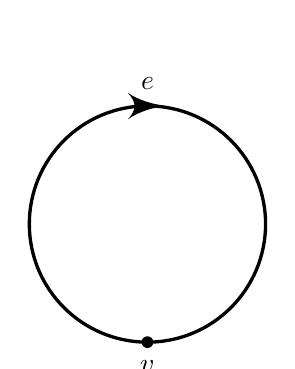
\begin{tikzpicture}[scale=1.5]
      \draw[-->] (90:1) arc[start angle=90, end angle=-270, radius=1];
      \node[fill, circle, inner sep=1.5pt, label=below:$v$] (v) at (0,-1) {};
      \node[inner sep=1.5pt, label=above:$e$] (e) at (0,1) {};
    \end{tikzpicture}
  \end{center}
  with the maps
  \begin{gather*}
    v \colon \Delta^0 \to S^1 \\
    e \colon \Delta^1 \to S^1
  \end{gather*}
  where $v$ maps its point $\Delta^0$ to the vertex $v$ and
  $e$ maps its interval $\Delta^1 = [v_0,v_1]$ to the edge $e$.
\end{example}

\begin{remark}
  A nonexample of constructing $S^1$ is defining $\aleph$ different
  $\Delta^0$ simplicies for each point of $S^1$.
  The reason this is a nonexample, is because condition $(3)$
  from \Cref{def:sigma-complex} would imply any subset of $S^1$
  is open.
  Although this pathological structure is a nonexample of $S^1$
  with its standard topology, it is a completely valid $\Delta$-simplex
  of $S^1$ with the discrete topology.
\end{remark}

\begin{example}[$\Delta$-complex of $T^1$]
  Let $T = S^1 \times S^1$ be the standard torus.
  \begin{center}
    \begin{tikzpicture}
        \draw[pattern=north west lines,opacity=0.7,pattern color=green] (-2,-2) -- (-2,2) -- (2,2) -- cycle;
        \draw[pattern=dots,opacity=0.7,pattern color=pink] (-2,-2) -- (2,-2) -- (2,2) -- cycle;
        \draw[->-=4,red] (-2,2) -- (2,2);
        \draw[-<-=4,blue] (2,2) -- (2,-2);
        \draw[-<-=4,red] (2,-2) -- (-2,-2);
        \draw[->-=4,blue] (-2,-2) -- (-2,2);
        \draw[->>-={sqrt(32)}] (-2,-2) -- (2,2);
        \node[fill, circle, inner sep=1.5pt, label=left:$r$] (r1) at (-2,-2) {};
        \node[fill, circle, inner sep=1.5pt, label=right:$r$] (r2) at (2,2) {};
        \node[fill, circle, inner sep=1.5pt, label=right:$r$] (r3) at (2,-2) {};
        \node[fill, circle, inner sep=1.5pt, label=left:$r$] (r4) at (-2,2) {};
        \node[label=left:$e$] (e1) at (-2,0) {};
        \node[label=right:$e$] (e2) at (2,0) {};
        \node[label=above:$f$] (f1) at (0,2) {};
        \node[label=below:$f$] (f2) at (0,-2) {};
        \node[label=center:$V$] (V) at (-0.8,0.8) {};
        \node[label=center:$L$] (L) at (0.8,-0.8) {};
        \node[label=below right:$g$] (g) at (-0.2,0.2) {};
        \node[label=center:{\scalebox{4}{$\circlearrowleft$}}]
          (circ1) at (0.8,-0.8) {};
        \node[label=center:{\scalebox{4}{$\circlearrowright$}}]
          (circ2) at (-0.8,0.8) {};
    \end{tikzpicture}
  \end{center}
  This $\Delta$-complex of the torus is the collection of
  $r \colon \Delta^0 \to T$ and $e,f,g \colon \Delta^1 \to T$
  and $V,L \colon \Delta^2 \to T$ as can be seen in the diagram.
\end{example}

\begin{example}[$\Delta$-complex of $\RP^2$]
  \label{exmp:delta-complex-rp2}
  Let $\RP^2 := \D^2/\forall x \in S^1 : x \sim -x$ be the following space.
  \[
  \tikz[eqpic]{
        \draw[pattern=north west lines,opacity=0.7,pattern color=green] (-2,-2) -- (-2,2) -- (2,2) -- cycle;
        \draw[pattern=dots,opacity=0.7,pattern color=pink] (-2,-2) -- (2,-2) -- (2,2) -- cycle;
        \draw[-<-=4,red] (-2,2) -- (2,2);
        \draw[->-=4,blue] (2,2) -- (2,-2);
        \draw[-<-=4,red] (2,-2) -- (-2,-2);
        \draw[->-=4,blue] (-2,-2) -- (-2,2);
        \draw[->>-={sqrt(32)}] (-2,-2) -- (2,2);
        \node[fill, circle, inner sep=1.5pt, label=left:$r$] (r1) at (-2,-2) {};
        \node[fill, circle, inner sep=1.5pt, label=right:$r$] (r2) at (2,2) {};
        \node[fill, circle, inner sep=1.5pt, label=right:$w$] (r3) at (2,-2) {};
        \node[fill, circle, inner sep=1.5pt, label=left:$w$] (r4) at (-2,2) {};
        \node[label=left:$e$] (e1) at (-2,0) {};
        \node[label=right:$e$] (e2) at (2,0) {};
        \node[label=above:$f$] (f1) at (0,2) {};
        \node[label=below:$f$] (f2) at (0,-2) {};
        \node[label=center:$V$] (V) at (-0.8,0.8) {};
        \node[label=center:$L$] (L) at (0.8,-0.8) {};
        \node[label=below right:$g$] (g) at (-0.2,0.2) {};
        \node[label=center:{\scalebox{4}{$\circlearrowright$}}]
          (circ1) at (0.8,-0.8) {};
        \node[label=center:{\scalebox{4}{$\circlearrowleft$}}]
          (circ2) at (-0.8,0.8) {};
      } \quad \simeq \quad
    \tikz[eqpic]{
        \draw[pattern=north east lines,opacity=0.7,pattern color=green] (2,0) circle (2cm);
        \node[fill, circle, inner sep=1.5pt, label=above:$r$] (r1) at (2,2) {};
        \node[fill, circle, inner sep=1.5pt, label=below:$r$] (r2) at (2,-2) {};
        \node[label=left:$e$] (e1) at (0,0) {};
        \node[label=right:$e$] (e2) at (4,0) {};
        \node[label=center:$L$] (L) at (2,0) {};
        \draw[-->] (0,0) arc[start angle=-180, end angle=180, radius=2];
        \draw[-->] (0,0) arc[start angle=-180, end angle=360, radius=2];
    }
    \]
  This $\Delta$-complex of the real projective plane is the collection of
  $r,w \colon \Delta^0 \to \RP^2$ and $e,f,g \colon \Delta^1 \to \RP^2$
  and $V,L \colon \Delta^2 \to \RP^2$ as can be seen in the diagram.
  Notice that the right hand side is not a $\Delta$-complex,
  it is just the quotient space that represents the real projective
  plane.
\end{example}

\begin{remark}[Orienatation of the faces]
  \label{rem:order}
  In \Cref{exmp:delta-complex-rp2},
  we need to have all of the edges
  in the faces $V$, $L$, in a very specific order.
  For example if $V \colon [v_0,v_1,v_2] \to \RP^2$
  then by part $(2)$ of \Cref{def:sigma-complex}
  the maps $V\vert_{[v_0,v_1]}$, $V\vert_{[v_1,v_2]}$
  and $V\vert_{[v_0,v_2]}$ must all be part of the sigma complex.
  The circular arrows represent if the vertices $v_0$, $v_1$,
  and $v_2$ are order clockwise or counterclockwise.
  In this case the orientation of $V$ is counterclockwise and indeed
  $V\vert_{[v_0,v_1]} = g$, $V\vert_{[v_1,v_2]} = f$,
  and $V\vert_{[v_0,v_2]} = e$ so all the edges are in the $\Delta$-complex.
  If this weren't the case then this would not have been a $\Delta$-complex.
\end{remark}

\begin{remark}
  The space $X$ is determined by the data of the $\Delta$-complex.
  This means that the CW-complex of the generated by the $\Delta$-complex
  is homeomorphic to $X$.
\end{remark}

\begin{definition}[Simplicial complex]
  \label{def:simplicial-complex}
  A simplicial complex is a $\Delta$-complex so that each simplex
  $\sigma_{\alpha} \colon \Delta^n \to X$ is
  \begin{enumerate}
    \item[(1)] injective
      (it suffices to check that it is injective on the vertices).
    \item[(2)] $\sigma_{\alpha}$ is determined by its vertices.
  \end{enumerate}
\end{definition}

\begin{example}
  One of the simplest examples is the triangle.
  \begin{center}
  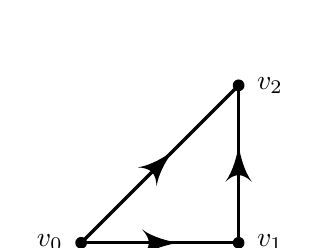
\begin{tikzpicture}
    \draw[->-=2] (0,0) -- (0,2);
    \draw[->-=2] (-2,0) -- (0,0);
    \draw[->-={sqrt(8)}] (-2,0) -- (0,2);
    \node[fill, circle, inner sep=1.5pt, label=left:$v_0$] (v0) at (-2,0){};
    \node[fill, circle, inner sep=1.5pt, label=right:$v_1$] (v1) at (0,0){};
    \node[fill, circle, inner sep=1.5pt, label=right:$v_2$] (v1) at (0,2){};
  \end{tikzpicture}
  \end{center}
\end{example}

\begin{example}
  The $\Delta$-complexes below are \textit{nonexamples}
  of simplicial complexes.
  \[
    \tikz[eqpic,scale=0.5]{
        \node[fill, circle, inner sep=1.5pt, label=below:$r$] (r) at (0,-4) {};
        \node[label=above:$e$] (e) at (0,0) {};
        \draw[-->] (0,0) arc[start angle=90, end angle=-270, radius=2];
    } \qquad
    \tikz[eqpic,scale=0.5]{
        \node[fill, circle, inner sep=1.5pt, label=above:$v_0$] (r1) at (2,2) {};
        \node[fill, circle, inner sep=1.5pt, label=below:$v_1$] (r2) at (2,-2) {};
        \node[label=left:$e$] (e) at (0,0) {};
        \node[label=right:$f$] (f) at (4,0) {};
        \draw[-->] (0,0) arc[start angle=-180, end angle=180, radius=2];
        \draw[-->] (0,0) arc[start angle=-180, end angle=360, radius=2];
    }
  \]
  The $\Delta$-complex on the left does not satisfy condition $(1)$
  in \Cref{def:simplicial-complex} since $e$ is not injective.
  The $\Delta$-complex on the right does not satisfy condition $(2)$
  in \Cref{def:simplicial-complex} since both $e$ and $f$ are not determined
  by their vertices.
\end{example}

\begin{remark}
  A simplicial complex is a generalization of simple graphes.
\end{remark}

\begin{remark}
  We can always cover any space by just using a vertex for any point in $X$,
  but this will be a $\Delta$-complex of $X$ endowed with the discrete
  topology.
\end{remark}

\subsection{Simplicial homology}
\begin{definition}[Chains]
  Let $X$ be a topological space with $\Delta$-structure
  $\set{\sigma_{\alpha}^{n_{\alpha}} \colon \Delta^{n_{\alpha}} \to X}_{\alpha}$.
  Then for any $n \geq 1$ we define the group $C_n^{\Delta}(X)$
  in one of the following ways:
  \begin{align*}
    C_n^{\Delta}(X) &:=
    \text{free abelian group with basis }\set{\sigma_{\alpha}^{n}}_{\alpha} \\ &:=
    \bigoplus \Z \sigma_{\alpha}^{n} \\ &:=
    \vspan_{\Z}\set{\sigma_{\alpha}^{n}} \\ &:=
    \set{\sum c_{\alpha} \sigma_{\alpha}^{n} \middle\vert c_{\alpha} \in \Z
    \text{ all but finitely many are $0$}}.
  \end{align*}
\end{definition}

\begin{remark}
  An element of $C_n^{\Delta}(X)$ is called an $n$-chain.
\end{remark}
 
\begin{example}[Chain in $S^1$]
  Consider the $\Delta$-complex we saw earlier
  \begin{center}
    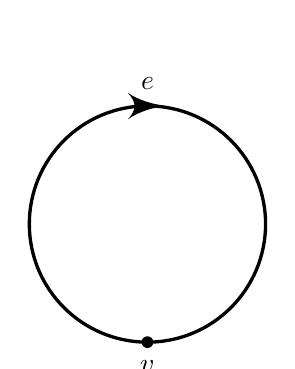
\begin{tikzpicture}[scale=1.5]
      \draw[-->] (90:1) arc[start angle=90, end angle=-270, radius=1];
      \node[fill, circle, inner sep=1.5pt, label=below:$v$] (v) at (0,-1) {};
      \node[inner sep=1.5pt, label=above:$e$] (e) at (0,1) {};
    \end{tikzpicture}
  \end{center}
  We have that $C_0^{\Delta}(S^1) = \Z v$ and that $C_1^{\Delta}(S^1) = \Z e$.
  For any $n \geq 2$ we have $C_n^{\Delta}(S^1) = \set{0}$.
\end{example}

\begin{definition}[Boundary map]
  We define the map $\partial_n \colon C_n^{\Delta}(X) \to C_{n-1}^{\Delta}(X)$
  on basis elements by
  \[
    \partial_n \sigma = \sum_{i=0}^{n} (-1)^{i} \sigma\vert_{\face{i}}
  \]
  and extend it linearly.
\end{definition}

\begin{remark}
  The boundary map is a group homomorphism.
\end{remark}

\begin{example}
  Consider the following as chains in some arbitrary $\Delta$-complex.
  \[
    \tikz[eqpic]{
      \node[fill, circle, inner sep=1.5pt, label=below:$v_0$] (v0) at (-2,0) {};
      \node[fill, circle, inner sep=1.5pt, label=below:$v_1$] (v1) at (0,0) {};
      \draw[->-=2] (-2,0) -- (0,0);
      \node[label=above:$e$] (e) at (-1,0) {};
    } \qquad
    \tikz[eqpic]{
      \draw[->-=2] (0,0) -- (0,2);
      \draw[->-=2] (-2,0) -- (0,0);
      \draw[->-={sqrt(8)}] (-2,0) -- (0,2);
      \node[fill, circle, inner sep=1.5pt, label=left:$v_0$] (v0) at (-2,0){};
      \node[fill, circle, inner sep=1.5pt, label=right:$v_1$] (v1) at (0,0){};
      \node[fill, circle, inner sep=1.5pt, label=right:$v_2$] (v1) at (0,2){};
      \node[label=center:{\scalebox{2}{$\circlearrowleft$}}]
        (circ) at (-0.6,0.6) {};
      \node[label=center:$\sigma$] (sigma) at (-0.6,0.6) {};
      \node[label=below:$e_2$] (e2) at (-1,0) {};
      \node[label=right:$e_0$] (e0) at (0,1) {};
      \node[label=left:$e_1$] (e1) at (-1,1) {};
    }
  \]
  Then the boundary of the $1$-chain ($e$) on the left is
  \[
    \partial(e) = \sigma\vert_{[v_1]} - \sigma\vert_{[v_0]} = v_1 - v_0,
  \]
  and the boundary of the $2$-chain ($\sigma$) on the right is
  \[
    \sigma(\sigma) =
    \sigma\vert_{[v_0,v_1]} +
    \sigma\vert_{[v_1,v_2]} -
    \sigma\vert_{[v_0,v_2]} = e_2 + e_0 - e_1.
  \]
  Notice that when we calculate the boundary of a chain we don't have do
  it by the formula, we just have to put a $-$ when the orientation of $\sigma$
  is opposite to the orientation of the edge for example.
\end{example}

\begin{example}
  Consider again the $\Delta$-complex of $S^1$.
  \begin{center}
    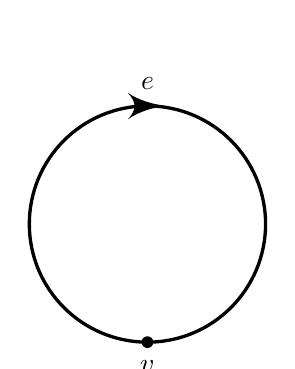
\begin{tikzpicture}[scale=1.5]
      \draw[-->] (90:1) arc[start angle=90, end angle=-270, radius=1];
      \node[fill, circle, inner sep=1.5pt, label=below:$v$] (v) at (0,-1) {};
      \node[inner sep=1.5pt, label=above:$e$] (e) at (0,1) {};
    \end{tikzpicture}
  \end{center}
  We already computed the chains in $S^1$ so we know that
  $\partial \colon \Z e \to \Z v$.
  However, we see that when $a \in Z$ that
  \[
    \sigma_1(ae) = a \sigma(e) = a(v - v) = 0,
  \]
  which implies that $\sigma_1 = 0$.
\end{example}

\begin{example}
  Consider again the $\Delta$-complex of the torus.
  \begin{center}
    \begin{tikzpicture}
        \draw[pattern=north west lines,opacity=0.7,pattern color=green] (-2,-2) -- (-2,2) -- (2,2) -- cycle;
        \draw[pattern=dots,opacity=0.7,pattern color=pink] (-2,-2) -- (2,-2) -- (2,2) -- cycle;
        \draw[->-=4,red] (-2,2) -- (2,2);
        \draw[-<-=4,blue] (2,2) -- (2,-2);
        \draw[-<-=4,red] (2,-2) -- (-2,-2);
        \draw[->-=4,blue] (-2,-2) -- (-2,2);
        \draw[->>-={sqrt(32)}] (-2,-2) -- (2,2);
        \node[fill, circle, inner sep=1.5pt, label=left:$r$] (r1) at (-2,-2) {};
        \node[fill, circle, inner sep=1.5pt, label=right:$r$] (r2) at (2,2) {};
        \node[fill, circle, inner sep=1.5pt, label=right:$r$] (r3) at (2,-2) {};
        \node[fill, circle, inner sep=1.5pt, label=left:$r$] (r4) at (-2,2) {};
        \node[label=left:$e$] (e1) at (-2,0) {};
        \node[label=right:$e$] (e2) at (2,0) {};
        \node[label=above:$f$] (f1) at (0,2) {};
        \node[label=below:$f$] (f2) at (0,-2) {};
        \node[label=center:$V$] (V) at (-0.8,0.8) {};
        \node[label=center:$L$] (L) at (0.8,-0.8) {};
        \node[label=below right:$g$] (g) at (-0.2,0.2) {};
        \node[label=center:{\scalebox{4}{$\circlearrowleft$}}]
          (circ1) at (0.8,-0.8) {};
        \node[label=center:{\scalebox{4}{$\circlearrowright$}}]
          (circ2) at (-0.8,0.8) {};
    \end{tikzpicture}
  \end{center}
  The structure of the boundary maps is
  \[\begin{tikzcd}
    {\set{0}} & {\Z V \oplus \Z L} & {\Z e \oplus \Z f \oplus \Z g} & {\Z r}
    \arrow["{\partial_3}", from=1-1, to=1-2]
    \arrow["{\partial_2}", from=1-2, to=1-3]
    \arrow["{\partial_1}", from=1-3, to=1-4]
  \end{tikzcd}\]
  We see that
  \begin{gather*}
    \partial_1(e) = r - r = 0 \\
    \partial_1(f) = r - r = 0 \\
    \partial_1(g) = r - r = 0
  \end{gather*}
  and
  \begin{gather*}
    \partial_2(V) = e + f - g \\
    \partial_2(L) = f + e - g
  \end{gather*}
\end{example}
\begin{remark}
  In the previous example when we computed the boundary of $V$,
  we did this by remembering that in a $\Delta$-complex a face
  is the image of a $2$-simplex $[v_0,v_1,v_2]$,
  which in the case of this complex are all sent to the same point,
  but from \Cref{rem:order} we know that the restriction of $V$
  to a face is already determined by the orientation of the edges,
  so that's how we know that $V\vert_{[v_0,v_1]} = -g$ etc.
\end{remark}

% to be added
% \begin{example}
%   In $\RP^2$ as we saw earlier we have
%   \[
%     \begin{tikzcd}
%       C_2 \arrow[r, "\partial_2"] & C_1 \arrow[r, "\partial_1"] & C_0
%     \end{tikzcd}
%   \]
% \end{example}

\begin{lemma}
  \label{lem:partial-partial-zero}
  We have that $\partial_{n-1} \circ \partial_{n} = 0$.
\end{lemma}
\begin{proof}
  First we check for basis elements.
  Let $\sigma \in C_{n+1}(X)$ be so that
  $\sigma \colon [v_0,\dots,v_{n}] \to X$.
  By definition we have that
  \[
    \partial_n \sigma = \sum_{i=0}^{n} (-1)^{i} \sigma\vert_{\face{i}}
  \]
  which implies that $(\partial_{n-1} \circ \partial_{n})(\sigma)$ is equal
  to
  \begin{multline*}
    \sum_{i=0}^{n} (-1)^{i} \partial_{n-1}\del{\sigma\vert_{\face{i}}} \\ =
    \sum_{i=0}^{n} (-1)^{i}
    \del{
    \sum_{j < i} (-1)^{j}
    \sigma\vert_{[v_0,\dots,\hat{v}_j,\dots,\hat{v}_j,\dots,v_n]} +
    \sum_{j > i} (-1)^{j-1}
    \sigma\vert_{[v_0,\dots,\hat{v}_j,\dots,\hat{v}_j,\dots,v_n]}
    }
  \end{multline*}
  but this is just equal to
  \[
    \sum_{j < i} (-1)^{i} (-1)^{j}
    \sigma\vert_{[v_0,\dots,\hat{v}_j,\dots,\hat{v}_j,\dots,v_n]} -
    \sum_{j > i} (-1)^{i} (-1)^{j}
    \sigma\vert_{[v_0,\dots,\hat{v}_j,\dots,\hat{v}_j,\dots,v_n]} = 0
  \]
\end{proof}

\begin{definition}[Cycles]
  We define the set of cycles to be $Z_n^{\Delta}(X) = \ker \partial_n$.
  Elements in $Z_n^{\Delta}(X)$ are called cycles or $n$-cycles.
\end{definition}

\begin{definition}[Boundaries]
  We define the set of boundaries to be $B_n^{\Delta}(X) = \im \partial_n$.
  Elements in $B_n^{\Delta}(X)$ are called boundaries.
\end{definition}

\begin{corollary}
  From \Cref{lem:partial-partial-zero}
  we have that $B^{\Delta}_{n+1}(X) \subseteq Z^{\Delta}_{n}(X)$.
  % we also have Z_n \subset C_n
\end{corollary}

\begin{definition}[Homology]
  We define the $n$th homology to be
  $H^{\Delta}_n(X) = Z^{\Delta}_n(X) / B^{\Delta}_{n+1}(X)$.
  The elements of $H^{\Delta}_n(X)$ are called homology classes.
\end{definition}
\[\begin{tikzcd}[ampersand replacement=\&,cramped]
	0 \& \Z \& {\Z^3} \& {\Z^3} \& 0
	\arrow[from=1-1, to=1-2]
	\arrow["{\partial_2}", from=1-2, to=1-3]
	\arrow["{\partial_1}", from=1-3, to=1-4]
	\arrow[from=1-4, to=1-5]
\end{tikzcd}\]
\begin{definition}[Homologous cycles]
  Let $z_1,z_2 \in Z_n(X)$ be cycles.
  Then we denote $z_1 \sim z_2$ and say that $z_1$ and $z_2$ are homologous
  if $[z_1] = [z_2] \in H_n(X)$.
  This is equivalent to saying $z_1 - z_2 \in B_n(X)$ etc.
  These equivalency classes are somtimes called homology classes.
\end{definition}

% examples?
% \begin{definition}
%   Two
%   \[\begin{tikzcd}
%     C_2 \arrow[r, "\partial_2"] & C_1 \arrow[r, "\partial_1"] & C_0
%   \end{tikzcd}\]
% \end{definition}

% more examples

% \begin{example}
%   Consider $X = T^2$ with the following diagram
%   \begin{center}
%     \begin{tikzpicture}
%       \begin{scope}[very thick, every node/.style={sloped,allow upside down}]
%       \end{scope}
%   \end{tikzpicture}
%   \end{center}
%   we have that
%   \[
%     0 \to C_2(X) \to C_1(X) \to C_0(X) \to 0
%   \]
% \end{example}

\begin{remark}
  In general we get that $H^1(X)$ is the abelianization of $\pi_1(X)$.
  We will see what this means later.
\end{remark}

\subsection{Singular homology}
\begin{definition}[Singular $n$-simplex]
  Let $X$ be a topological space.
  A singular $n$-simplex is a continuous map $\sigma \colon \Delta^n \to X$.
\end{definition}

\begin{remark}
  In order to define singular homology we need to define chains
  and boundaries again.
  We define
  \[
    C_n(X) := \set{\text{the free abelian group with basis the set of singular
    $n$-simplices}}.
  \]
  We call elements in $C_n(X)$ singular $n$-chains.
  Take a moment to appreciate how big this groups is.
  The boundary map $\partial_n$ is defined similarly,
  \[
    \partial_n(\sigma) :=
    \sum_{i} (-1)^{i} \sigma\vert_{\face{i}}
  \]
  and cycles ($Z_n$), boundaries ($B_n$) and homology ($H_n = Z_n/B_n$)
  are defined in a similar way to how we defined them in simplicial homology
  as well.
\end{remark}

\begin{lemma}
  Let $X = \set{*}$.
  Then 
  \[
    H_n(X) =
    \begin{cases}
      \Z, &n = 0, \\
      0, &n \geq 1.
    \end{cases}
  \]
\end{lemma}
\begin{proof}
  For any $n \geq 1$ we see that
  \[
    C_n(X) = \Z \sigma^n
  \]
  where $\sigma^n$ is the constant map $[v_0,\dots,v_n] \to \set{*}$.
  When $n = 0$ we also have that $\partial_0(\sigma^0) = 0$ and if $n \geq 1$
  then
  \[
    \partial_n \sigma^n =
    \sum_{i=0}^{n} (-1)^{i}
    \underbrace{\sigma\vert_{\face{i}}}_{\sigma^{n-1}} =
    \begin{cases}
      \sigma^{n-1}, &n \text{ even}, \\
      0, &n \text{ odd}.
    \end{cases}
  \]
  We have that
  \[
    \begin{tikzcd}
	\cdots & {C_3(\set{*})} & {C_2(\set{*})} & {C_1(\set{*})} & {C_0(\set{*})} & 0 \\
	\cdots & \Z & \Z & \Z & \Z & 0
	\arrow[from=1-1, to=1-2]
	\arrow[from=1-2, to=1-3]
	\arrow["{\rotatebox{90}{=}}"{description}, draw=none, from=1-2, to=2-2]
	\arrow[from=1-3, to=1-4]
	\arrow["{\rotatebox{90}{=}}"{description}, draw=none, from=1-3, to=2-3]
	\arrow[from=1-4, to=1-5]
	\arrow[from=1-5, to=1-6]
	\arrow["{\rotatebox{90}{=}}"{description}, draw=none, from=1-4, to=2-4]
	\arrow["{\rotatebox{90}{=}}"{description}, draw=none, from=1-5, to=2-5]
  \arrow["{\rotatebox{90}{=}}"{description}, draw=none, from=1-6, to=2-6]
	\arrow[from=2-1, to=2-2]
	\arrow[from=2-2, to=2-3]
	\arrow[from=2-3, to=2-4]
	\arrow[from=2-4, to=2-5]
	\arrow[from=2-5, to=2-6]
    \end{tikzcd}
  \]
  and then we have that
  \[
    H_0(X) =
    \frac{\ker \partial_0}{\im \partial_1} =
    \frac{\Z}{\set{0}} \cong \Z
  \]
  and for $n \geq 1$ we have one of the following
  \[
    H_n(X) =
    \frac{\ker \partial_{n}}{\im \partial_{n+1}} =
    \frac{\Z}{\Z} \cong \set{0} \tor
    H_n(X) =
    \frac{\ker \partial_{n}}{\im \partial_{n+1}} =
    \frac{\set{0}}{\set{0}} \cong \set{0}
  \]
  which completes the proof.
\end{proof}

\begin{remark}
  Let $X$ and $Y$ be homeomorphic spaces.
  Then $H_n(X) \cong H_n(Y)$.
\end{remark}

\begin{lemma}
  Let $X = \bigsqcup X_{\alpha}$ where $X_{\alpha}$ are the connected
  components of $X$.
  Then $H_n(X) = \bigoplus_{\alpha} H_n(X_{\alpha})$
\end{lemma}
\begin{proof}
  The intuition behind this lemma is that since each
  $\sigma \colon \Delta^n \to X$ must be continuous, it must
  only exist within a single unique path component of $\bigsqcup X_{\alpha}$.
  This intuition is enough justification for us to say that
  \[
    C_n(X) = \bigoplus_{\alpha} C_n(X_{\alpha}).
  \]
  For each $\sigma \in C_n(X_{\alpha})$ we have that
  $\partial_n \sigma \in C_{n-1}(X_{\alpha})$
  which implies that
  \begin{gather*}
    Z_n(X) = \ker \partial_n = \bigoplus_{\alpha} Z_n(X_{\alpha}) \\
    B_n(X) = \im \partial_{n+1} = \bigoplus_{\alpha} B_n(X_{\alpha})
  \end{gather*}
  which implies that
  \[
    H_n(X_{\alpha}) = Z_n / B_n = \bigoplus_{\alpha} H_n(X_{\alpha})
  \]
  which completes the proof.
\end{proof}

\begin{lemma}
  \label{lem:path-connected-then-hzero-z}
  Let $X$ be path connected.
  Then $H_0(X) \cong \Z$.
\end{lemma}
\begin{proof}
  We have that
  \[
    H_0(X) =
    \frac{\ker \partial_0}{\im \partial_1}
  \]
  where $\ker \partial_0 = C_0(X)$ is all maps $\sigma \colon \Delta^0 \to X$
  and $\im \partial_1$ is the difference of any two points in $X$
  (because each two points can be connected by a path)
  and thus clearly
  \[
    H_0(X) =
    \frac{\ker \partial_0}{\im \partial_1} \cong \Z
  \]
  which is generated by any map $\sigma \colon \Delta^0 \to X$
  (all other maps are equal to it after modding by $\im \partial_1$).
\end{proof}

\begin{corollary}
  Let $X$ be a topological space.
  Then $H_0(X)$ is the direct sum of $\Z$'s, one for each path-component
  of $X$.
\end{corollary}

\begin{remark}
  Before getting into homotopy invariance, let us consider
  a different, more rigorous proof for \Cref{lem:path-connected-then-hzero-z}
  that will give us more motivation for reduced homology.
\end{remark}

\begin{proofof}{\Cref{lem:path-connected-then-hzero-z}}
  We have that
  \[\begin{tikzcd}
	{} & {C_1(X)} & {C_0(X)} & 0
	\arrow[from=1-1, to=1-2]
	\arrow["{\partial_1}", from=1-2, to=1-3]
	\arrow[from=1-3, to=1-4]
\end{tikzcd}\]
  so $\partial_0 = 0$ which means that
  \[
    H_0(X) =
    \frac{\ker \partial_0}{\im \partial_1} =
    \frac{C_0(X)}{\im \partial_1}.
  \]
  We now define a new map $\epsilon \colon C_0(X) \to \Z$ by
  \[
    \epsilon\del[4]{\sum_i n_i \sigma_i} = \sum_{i=1}^{n} n_i.
  \]
  This map is obviously surjective if $X$ is nonempty.
  If we show that $\ker \epsilon = \im \partial_1$ then by the first
  isomorphism theorem we would have
  \[
    H_0(X) =
    \frac{C_0(X)}{\im \partial_1} =
    \frac{C_0(X)}{\ker \epsilon} \cong \Z.
  \]
  First we observe that $\im \partial_1 \subset \ker \epsilon$
  since for a singular $1$-simplex (a path) we have
  \[
    \epsilon \del{\partial_1(\sigma)} =
    \epsilon \del{\sigma_{[v_1]} - \sigma_{[v_0]}} = 1 - 1 = 0.
  \]
  It is left to show that $\ker \epsilon \subset \im \partial_1$.
  Let $\sum_i n_i \sigma_i \in \ker \epsilon$.
  This means that
  \[
    \epsilon\del[4]{\sum_i n_i \sigma_i} = \sum_i n_i = 0.
  \]
  Since the $\sigma_i$ are singular $0$-simplices they are simply
  constant maps to points of $X$.
  We can define a path $\tau_i \colon [0,1] \to X$ from a basepoint $x_0$
  to $\sigma_i([v_0])$ and set $\sigma_0$ to be the singular $0$-simplex with
  image $x_0$.
  We can consider $\tau_i$ as singular $1$-simplices,
  maps $\tau_i \colon [v_0,v_1] \to X$,
  and then we have $\partial(\tau_i) = \sigma_i - \sigma_0$.
  So since $\sum_i n_i = 0$
  \[
    \partial_1\del[4]{\sum_i n_i \tau_i} =
    \sum_i n_i \sigma_i - \sum_i n_i \sigma_0 =
    \sum_i n_i \sigma_i.
  \]
  Thus $\sum_i n_i \sigma_i \in \im \partial_1$, which shows that
  $\ker \epsilon \subset \im \partial_1$ and completes the proof.
\end{proofof}

\begin{definition}[Chain complex]
  A chain complex is a sequence
  \[\begin{tikzcd}
	\cdots & {A_2} & {A_1} & {A_0} & \cdots
	\arrow[from=1-1, to=1-2]
	\arrow["{\partial_2}", from=1-2, to=1-3]
	\arrow["{\partial_1}", from=1-3, to=1-4]
	\arrow["{\partial_0}", from=1-4, to=1-5]
\end{tikzcd}\]
  where $A_n$ are abelian groups such that
  $\partial_n \circ \partial_{n+1} = 0$.
\end{definition}
\begin{remark}
  We sometimes denote $\partial_n \circ \partial_{n+1} = 0$
  as $\partial^2 = 0$.
\end{remark}
\begin{remark}
  The equation $\partial_n \circ \partial_{n+1} = 0$ is equivalent
  to the inclusion $\im \partial_{n+1} \subset \ker \partial_{n}$.
\end{remark}

\begin{remark}
  Earlier in the alternative proof
  for \Cref{lem:path-connected-then-hzero-z}
  we saw (although we didn't mention it directly) the augumented chain complex
  \[\begin{tikzcd}
    \cdots & {C_2(X)} & {C_1(X)} & {C_0(X)} & \Z & 0
    \arrow[from=1-1, to=1-2]
    \arrow["{\partial_2}", from=1-2, to=1-3]
    \arrow["{\partial_1}", from=1-3, to=1-4]
    \arrow["\epsilon", from=1-4, to=1-5]
    \arrow[from=1-5, to=1-6]
  \end{tikzcd}\]
  which is called the reduced chain complex.
\end{remark}

\begin{definition}[Reduced homology groups]
  We define the reduced homology groups $\widetilde{H}_n(X)$ as the
  homology groups of the augmented chain complex
  \[\begin{tikzcd}
    \cdots & {C_2(X)} & {C_1(X)} & {C_0(X)} & \Z & 0
    \arrow[from=1-1, to=1-2]
    \arrow["{\partial_2}", from=1-2, to=1-3]
    \arrow["{\partial_1}", from=1-3, to=1-4]
    \arrow["\epsilon", from=1-4, to=1-5]
    \arrow[from=1-5, to=1-6]
  \end{tikzcd}\]
  where $\epsilon$ is the map we saw
  in \Cref{lem:path-connected-then-hzero-z}.
  In this reduced way of computing homoloy,
  a point has trivial homology groups in all dimensions.
  We also want to require $X$ to be nonempty
  to avoid having a nontrivial homology group in dimension $-1$.
\end{definition}

\begin{remark}
  We have that
  \[
    H_n(X) =
    \begin{cases}
      \widetilde H_n(X), &\forall n \geq 1, \\
      \widetilde H_0(X) \oplus \Z, &n=0,
    \end{cases}
  \]
  since $\widetilde{H}_0(X) = 0$ where $X$ is path connected.
\end{remark}
\begin{remark}
  In order to show that $H_0(X) = \widetilde{H}_0(X) \oplus \Z$ we notice that
  $\epsilon$ induces a map $\epsilon \colon H_0(X) \to \Z$
  whose kernel is in $\widetilde{H}_0(X)$.
  After some manipulations we get that
  $H_0(X) = \widetilde{H}_0(X) \oplus \Z$ as wanted.
\end{remark}

\begin{remark}
  Formally, we can think of the extra $\Z$ in the augumented chain complex
  as generated by the unique map $[\emptyset] \to X$ where $[\emptyset]$
  is the empty simplex, which no vertices.
  The augumentation map $\epsilon$ is then the usual boundary map
  since $\partial[v_0] = [\hat v_0] = [\emptyset]$.
\end{remark}

\begin{remark}[Geometric interpretation]
  Let $c = \sum n_{\sigma} \sigma \in Z_n(X)$ be a cycle.
  For example we can take $c = \sum n_{e} e \in Z_1(X)$.
  Since $0 = \partial c$,
  every endpoint of a $1$-simplex cancels out with an initial point
  of a $1$-simplex.
  This means that every such point will look somewhat like the following:
  \begin{center}
    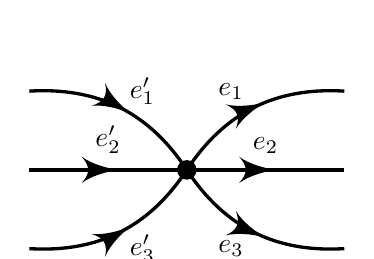
\begin{tikzpicture}
      \draw[->-=4] (-2,1) to[bend left=30]  (0,0);
      \draw[->-=4] (-2,-1) to[bend right=30] (0,0);
      \draw[->-=4] (-2,0) -- (0,0);
      \draw[->-=4] (0,0) to[bend left=30]  (2,1);
      \draw[->-=4] (0,0) to[bend right=30] (2,-1);
      \draw[->-=4] (0,0) -- (2,0);
      \node[fill, circle, inner sep=2.5] (v) at (0,0) {};
      \node[label=left:$e_1$] at (1,1) {};
      \node[inner sep=1.5pt,label=above:$e_2$] at (1,0) {};
      \node[label=left:$e_3$] at (1,-1) {};
      \node[label=right:$e'_1$] at (-1,1) {};
      \node[inner sep=1.5pt,label=above:$e'_2$] at (-1,0) {};
      \node[label=right:$e'_3$] at (-1,-1) {};
    \end{tikzpicture}
  \end{center}
  Students who major in physics may appreciate that if we define the chain
  groups to be the span of the singular simplices over $\R$ instead of $\Z$,
  this looks a lot like Kirchhoff's second law.
  Moreover, when at every point the amount of edges coming in and going
  out is equal, the chain is necessarily a cycle, and even a closed
  $1$-manifold.
  Similarly, we can consider $c \in Z_2(X)$ which is a closed
  topological surface. That it because, it is a cycle precisely if
  and only if it has no boundary.
  When we consider a chain that is not a cycle,
  we get manifolds with boundary.
  For reasons beyond my comprehension,
  this argument does not work in higher dimensions
  and we only get psuedo-manifolds.
\end{remark}

\subsection{Homotopy invariance}

\begin{definition}
  Let $f \colon X \to Y$ be a continuous map.
  Then for every $\sigma \colon \Delta^n \to X$ the map
  induces a new map $f \circ \sigma \colon \Delta^n \to Y$.
  Let $f_{\#} \colon C_n(X) \to C_n(Y)$ be the map defined on basis
  elements by $f_{\#}(\sigma) = f \circ \sigma$.
  This gives us the following diagram
  \[\begin{tikzcd}
	\cdots & {C_{n+1}(X)} & {C_n(X)} & {C_{n-1}(X)} & \cdots \\
	\cdots & {C_{n+1}(Y)} & {C_n(Y)} & {C_{n-1}(Y)} & \cdots
	\arrow[from=1-1, to=1-2]
	\arrow["\partial", from=1-2, to=1-3]
  \arrow["{f_{\#}}", from=1-2, to=2-2]
	\arrow["\partial", from=1-3, to=1-4]
  \arrow["{f_{\#}}", from=1-3, to=2-3]
	\arrow[from=1-4, to=1-5]
	\arrow["{f_{\#}}", from=1-4, to=2-4]
	\arrow[from=2-1, to=2-2]
	\arrow["\partial", from=2-2, to=2-3]
	\arrow["\partial", from=2-3, to=2-4]
	\arrow[from=2-4, to=2-5]
\end{tikzcd}\]
\end{definition}

\begin{proposition}
  The map $f_{\#}$ commutes with $\partial$.
  That is, $f_{\#} \circ \partial = \partial \circ f_{\#}$.
  This is equivalent to saying that the diagram
  \[\begin{tikzcd}
	\cdots & {C_{n+1}(X)} & {C_n(X)} & {C_{n-1}(X)} & \cdots \\
	\cdots & {C_{n+1}(Y)} & {C_n(Y)} & {C_{n-1}(Y)} & \cdots
	\arrow[from=1-1, to=1-2]
	\arrow["\partial", from=1-2, to=1-3]
  \arrow["{f_{\#}}", from=1-2, to=2-2]
	\arrow["\partial", from=1-3, to=1-4]
  \arrow["{f_{\#}}", from=1-3, to=2-3]
	\arrow[from=1-4, to=1-5]
	\arrow["{f_{\#}}", from=1-4, to=2-4]
	\arrow[from=2-1, to=2-2]
	\arrow["\partial", from=2-2, to=2-3]
	\arrow["\partial", from=2-3, to=2-4]
	\arrow[from=2-4, to=2-5]
\end{tikzcd}\]
  commutes.
\end{proposition}
\begin{proof}
  In the homework.
\end{proof}

\begin{definition}[Chain map]
  The collection of maps $f_{\#}$ is called a chain map.
  Any map similar to $f_{\#}$ that commutes with the boundary operator
  is called a chain map.
\end{definition}

\begin{proposition}
  A chain map $f_{\#}$ induces a
  well defined map homomorphism $f_* \colon H_n(X) \to H_n(Y)$.
\end{proposition}
\begin{proof}
  Let $c \in Z_n(X)$ (this means that $\partial c = 0$).
  Then since we have
  \[
    \partial f_{\#} (c) =
    f_{\#} (\partial c) =
    f_{\#} (0) = 0,
  \]
  we get that $f_{\#}(c) \in Z_n(Y)$.
  Similarly for $b \in B_n(X)$ (which means that $b = \partial c$)
  we get that
  \[
    f_{\#}(b) =
    f_{\#} \del{\partial c} =
    \partial \del{f_{\#}(c)},
  \]
  so since $f_{\#}(c) \in C_{n+1}(Y)$ we have $f_{\#}(b) \in B_n(Y)$.
  Thus $f_{\#}$ induces a well defined homomorphism
  $f_* \colon H_n(X) \to H_n(Y)$ which completes the proof.
  The proof that this is indeed a homomorphism is omitted.
\end{proof}
\begin{remark}
  The homomorphism $f_{*}$ is called the induced map of $f$.
\end{remark}

\begin{proposition}[Functoriality of the induced map]
  \label{prp:functoriality-of-induced-maps}
  The induced map satisfies the following two properties
  for a chain complex
  \[\begin{tikzcd}
	X & Y & Z
	\arrow["g", from=1-1, to=1-2]
	\arrow["f", from=1-2, to=1-3]
\end{tikzcd}\]
  \begin{enumerate}
    \item[(1)] $(fg)_* = f_* g_*$;
    \item[(2)] $\mathbbm{1}_{*} = \mathbbm{1}$ where $\mathbbm{1}$ is the
      identity map of a space or a group.
  \end{enumerate}
\end{proposition}
\begin{corollary}
  Let $X$ and $Y$ be homeomorphic topological spaces.
  Then $H_n(X) \cong H_n(Y)$.
\end{corollary}

\begin{corollary}
  \label{cor:injective-i-surjective-r}
  Let $A \subseteq X$ be a retract of $X$.
  Then $i_* \colon H_n(A) \to H_n(X)$ is injective and
  $r_* \colon H_n(X) \to H_n(A)$ is surjective.
\end{corollary}
\begin{proof}
  We have the maps
  \[\begin{tikzcd}[ampersand replacement=\&,cramped]
    X \& A \\
    A
    \arrow["r", from=1-1, to=1-2]
    \arrow["i", from=2-1, to=1-1]
    \arrow["{r \circ i}"', from=2-1, to=1-2]
  \end{tikzcd}\]
  where $r \circ i = \id$ and then from \Cref{prp:functoriality-of-induced-maps}
  we get
  \[\begin{tikzcd}[ampersand replacement=\&,cramped]
    {H_n(X)} \& {H_n(A)} \\
    {H_n(A)}
    \arrow["{r_*}", from=1-1, to=1-2]
    \arrow["{i_*}", from=2-1, to=1-1]
    \arrow["{(\id)_*}"', from=2-1, to=1-2]
  \end{tikzcd}\]
  which implies that
  $r_* \circ i_* = (r \circ i)_* = (\id)_* = \id_{H_n(A)}$.
  This shows that $r_*$ must be surjective and $i_*$
  must be injective and completes the proof.
\end{proof}

\begin{corollary}
  $\set{0,1} \subseteq [0,1]$ is not a retract.
\end{corollary}
\begin{proof}
  Assume by contradiction that $\set{0,1} \subseteq [0,1]$ is a retract.
  Then by \Cref{cor:injective-i-surjective-r}
  the map $i_* \colon H_0\del{\set{0,1}} \to H_0\del{[0,1]}$ must be injective.
  However we know these homology groups so we get that
  $i_* \colon \Z \oplus \Z \to \Z$ must be injective.
  This contradiction completes the proof.
\end{proof}

\begin{theorem}
  \label{thm:homotopic-maps-induce-same-homomorphism-on-homology}
  Let $f,g \colon X \to Y$ be homotopic, that is, $f \simeq g$.
  Then the induced maps $f_*,g_* \colon H_n(X) \to H_n(Y)$ are equal
  for all $n \geq 0$.
\end{theorem}

\begin{definition}[Homotopy equivalence]
  Let $X$ and $Y$ be topological spaces.
  A continuous map $f \colon X \to Y$ is a homotopy equivalence if
  there exists a continuous map $g \colon Y \to X$ such that
  \[
    f \circ g \simeq \id_Y \tand
    g \circ f \simeq \id_X.
  \]
  If there exists a homotopy equivalence between $X$ and $Y$
  they are said to be homotopy equivalent (or that they have the same
  homotopy type), and we denote $X \simeq Y$.
\end{definition}
\begin{corollary}
  \label{cor:homotopy-equivalent-implies-same-homology}
  Let $X \simeq Y$.
  Then $H_n(X) \cong H_n(Y)$.
\end{corollary}
\begin{proof}
  In the homework.
\end{proof}

\begin{example}
  We can show that $\R^n \simeq \set{*}$ since we can take the maps
  \begin{align*}
    \begin{cases}
      f \colon \R^n \mapsto \set{*}, \\
      g \colon \set{*} \to 0.
    \end{cases}
  \end{align*}
  Then by \Cref{cor:homotopy-equivalent-implies-same-homology} we get that
  \[
    H_n\del{\R^n} =
    H_n\del{\set{*}} =
    \begin{cases}
      \Z &n = 0, \\
      0 &n \geq 1.
    \end{cases}
  \]
\end{example}
\begin{remark}
  So far we barely know anything about singular homology.
  We go back to prove
  \Cref{thm:homotopic-maps-induce-same-homomorphism-on-homology}
  in order to develop our tool set.
\end{remark}

\begin{proofof}{\Cref{thm:homotopic-maps-induce-same-homomorphism-on-homology}}
  We are going to build a chain homotopy $P \colon C_n(X) \to C_{n+1}(Y)$
  such that
  \[\begin{tikzcd}
	\cdots & {C_{n+1}(X)} & {C_{n}(X)} & {C_{n-1}(X)} & \cdots \\
	\cdots & {C_{n+1}(Y)} & {C_{n}(Y)} & {C_{n-1}(Y)} & \cdots
	\arrow[from=1-1, to=1-2]
	\arrow["\partial", from=1-2, to=1-3]
  \arrow["{g_{\#} - f_{\#}}"', from=1-2, to=2-2]
	\arrow["\partial", from=1-3, to=1-4]
	\arrow["P"', from=1-3, to=2-2]
	\arrow["{g_{\#} - f_{\#}}"', from=1-3, to=2-3]
	\arrow[from=1-4, to=1-5]
	\arrow["P"', from=1-4, to=2-3]
	\arrow["{g_{\#} - f_{\#}}"', from=1-4, to=2-4]
	\arrow[from=2-1, to=2-2]
	\arrow["\partial", from=2-2, to=2-3]
	\arrow["\partial", from=2-3, to=2-4]
	\arrow[from=2-4, to=2-5]
\end{tikzcd}\]
  and $g_{\#} - f_{\#} = \partial P + P \partial$.
  A map satisfying the above properties is called a \textit{chain homotopy}.
  Assuming chain homotopy $P$ exists we can show that $f_{*} = g_{*}$.
  First we notice that $P \colon C_n(X) \to C_{n+1}(Y)$.
  Let $c \in \ker \partial_n$.
  We then have
  \[
    \underbrace{\partial P(c) +
    \overbrace{P \partial(c)}^{=\,0}}_{g_{\#}(c) - f_{\#}(c)} =
    \partial P(c) \in \im \partial_{n+1}
  \]
  which implies that $g_* - f_*$ is the zero map since
  \[
    f_*(c) - g_*(c) = 0 \in H_n(Y) = Z_n(Y) / B_n(Y).
  \]
  Note that in general whenever $g_{\#} - f_{\#} = \partial P + P \partial$
  we get that $g_* = f_*$.
  The map we are going to construct $P$ is called the prism map.
  Our goal is $\partial P + P \partial = g_{\#} - f_{\#}$.
  Since $f$ and $g$ are homotopic there exists a homotopy
  $H \colon X \times [0,1] \to Y$ such that
  $H(x,0) = f(x)$ and $H(x,1) = g(x)$.
  In general when we construct the map $f_{\#}$ we have
  \[\begin{tikzcd}[ampersand replacement=\&,cramped]
    X \& Y \\
    {\Delta^n}
    \arrow["f", from=1-1, to=1-2]
    \arrow["\sigma", from=2-1, to=1-1]
    \arrow["{f \circ \sigma}"', from=2-1, to=1-2]
  \end{tikzcd}\]
  and we can see how the homotopy naturally induces a similar diagram
  \[\begin{tikzcd}[ampersand replacement=\&,cramped]
    {X \times [0,1]} \& \& Y \\ \\
    {\Delta^n \times [0,1]}
    \arrow["H", from=1-1, to=1-3]
    \arrow["{\sigma \times [0,1]}", from=3-1, to=1-1]
    \arrow["{H \circ \del{\sigma \times [0,1]}}"', from=3-1, to=1-3]
  \end{tikzcd}\]
  The object $\Delta^n \times [0,1]$ turns out to be
  a union of $n+1$ copies of $\Delta^{n+1}$.
  If we denote $[v_0,v_1,\dots,v_n]$ as the vertices
  of $\Delta^n \times \set{0}$ and $[w_0,w_1,\dots,w_n]$ as the vertices
  of $\Delta^n \times \set{1}$, these simplices can be written
  as $\Delta^{n+1}_i = [v_0,\dots,v_i,w_i,\dots,w_n]$ for
  $0 \le i \le n$.
  This gives rise to the following definition of
  $P \colon C_n(X) \to C_{n+1}(Y)$. For $\sigma \in C_n(X)$ let
  \[
    P(\sigma) = \sum_{i=0}^{n} (-1)^{i} H \circ (\sigma \times \id)
      \vert_{[v_0,\dots,v_i,w_i,\dots,w_n]}.
  \]
  We now compute $\partial P(\sigma)$.
  \begin{align*}
      \partial P(\sigma) &=
    \sum_{i=0}^{n} (-1)^{i} \partial \del{H \circ (\sigma \times \id)
      \vert_{[v_0,\dots,v_i,w_i,\dots,w_n]}} \\ &=
      \sum_{j \le i}^{n} (-1)^{i} (-1)^{j} H \circ (\sigma \times \id)
      \vert_{[v_0,\dots,\hat{v}_j,\dots,v_i,w_i,\dots,w_n]} \\ &+
      \sum_{j \geq i}^{n} (-1)^{i} (-1)^{j+1} H \circ (\sigma \times \id)
      \vert_{[v_0,\dots,v_i,w_i,\dots,\hat{w}_j,\dots,w_n]}.
  \end{align*}
  When $i = j$ the summands almost cancel out as we see below.
  \[
    (-1)^{0} (-1)^{0}
    \underbrace{H \circ \del{\sigma \times \id}\vert_{[w_0,\dots,w_n]}}_{g_{\#}(\sigma)} +
    (-1)^{n} (-1)^{n+1}
    \underbrace{H \circ \del{\sigma \times \id}\vert_{[v_0,\dots,v_n]}}_{f_{\#}(\sigma)} =
    g_{\#}(\sigma) - f_{\#}(\sigma).
  \]
  If we denote
  {\small \[
    (*) = \sum_{j < i}^{n} (-1)^{i} (-1)^{j} H \circ (\sigma \times \id)
      \vert_{[v_0,\dots,\hat{v}_j,\dots,v_i,w_i,\dots,w_n]} +
      \sum_{j > i}^{n} (-1)^{i} (-1)^{j+1} H \circ (\sigma \times \id)
      \vert_{[v_0,\dots,v_i,w_i,\dots,\hat{w}_j,\dots,w_n]}
  \]}
  This leaves us with
  \[
    \partial P(\sigma) = (*) + g_{\#}(\sigma) - f_{\#}(\sigma).
  \]
  In order to compute $P(\partial \sigma)$ we first notice that
  \[
    \partial \sigma = \sum_{i=0}^{n} (-1)^{i} \sigma\vert_{\face{i}}.
  \]
  We can now compute $P(\partial \sigma)$ as follows:
  \begin{align*} 
    P(\partial \sigma) &= \sum_{i=0}^{n} (-1)^{i} P\del{\sigma\vert_{\face{i}}} \\
                       &= (-1)
                       \Bigg(\sum_{j < i}^{n} (-1)^{i} (-1)^{j} H \circ (\sigma \times \id)
    \vert_{[v_0,\dots,\hat{v}_j,\dots,v_i,w_i,\dots,w_n]} \\ &\hspace{5em} +
      \sum_{j > i}^{n} (-1)^{i} (-1)^{j+1} H \circ (\sigma \times \id)
    \vert_{[v_0,\dots,v_i,w_i,\dots,\hat{w}_j,\dots,w_n]}\Bigg) \\ &= (-1)(*).
  \end{align*}
  It follows that
  \[
    \partial P + P \partial =
    (*) + g_{\#} - f_{\#} - (*) =
    g_{\#} - f_{\#}.
  \]
  This completes the proof.
\end{proofof}

\begin{corollary}
  Let $X$ be contractible.
  Then by \Cref{cor:homotopy-equivalent-implies-same-homology}
  it follows that $H_n(X) = H_n\del{\set{*}}$.
  Moreover,
  \[
    H_n\del{\set{*}} =
    \begin{cases}
      \Z, &n = 0, \\
      0, &n \neq 0.
    \end{cases}
  \]
\end{corollary}

\subsection{Exact sequences}

\begin{definition}[Exact sequence]
  A sequence of abelian groups (or any sequence of objects)
  \[\begin{tikzcd}
	\cdots & {A_{i+1}} & {A_i} & {A_{i-1}} & \cdots
	\arrow["{\alpha_{i+2}}", from=1-1, to=1-2]
	\arrow["{\alpha_{i+1}}", from=1-2, to=1-3]
	\arrow["\alpha_i", from=1-3, to=1-4]
	\arrow["{\alpha_{i-1}}", from=1-4, to=1-5]
  \end{tikzcd}\]
  is said to be exact if $\ker \alpha_{i} = \im \alpha_{i+1}$ for all $i$.
  If $\ker \alpha_{i} = \im \alpha_{i+1}$ for some $i$.
  then it is said to be exact at $A_i$.
\end{definition}
\begin{remark}
  A sequence is exact if and only if it is a chain complex with trivial
  homologies.
\end{remark}
\begin{remark}
  We call these sequences exact, because while usually we have that
  $\im \alpha_{n+1} \subseteq \ker \alpha_{n}$, here the image of
  $\alpha_{n+1}$ is \textit{exactly} the kernel of $\alpha_n$.
  This means that if $a \in A_n$ maps to zero then necessarily there
  exists $b \in A_{n+1}$ so that $\alpha_{n+1}(b) = a$.
  We also still have the property $\alpha_{n+1} \circ \alpha_{n} = 0$.
\end{remark}

\begin{example}
  The sequence
  \[\begin{tikzcd}
	0 & A & B
	\arrow[from=1-1, to=1-2]
	\arrow["\alpha", from=1-2, to=1-3]
  \end{tikzcd}\]
  is exact if and only if $\ker \alpha = 0$
  if and only if $\alpha$ is injective.
\end{example}
\begin{example}
  The sequence
  \[\begin{tikzcd}
	A & B & 0
	\arrow[from=1-2, to=1-3]
	\arrow["\beta", from=1-1, to=1-2]
  \end{tikzcd}\]
  is exact if and only if $\im \beta = B$
  if and only if $\beta$ is surjective.
\end{example}
\begin{example}
  \label{exmp:short-exact-sequence-isomorphism}
  We can combine the last two results and get that the sequence
  \[\begin{tikzcd}
  0 & A & B & 0
	\arrow[from=1-1, to=1-2]
	\arrow[from=1-2, to=1-3]
	\arrow[from=1-3, to=1-4]
	\arrow["\alpha", from=1-2, to=1-3]
  \end{tikzcd}\]
  is exact if and only if $\alpha$ is an isomorphism.
\end{example}

\begin{example}[Short exact sequence]
  A short exact sequence is an exact sequence of the form
  \[\begin{tikzcd}
	0 & A & B & C & 0
	\arrow[from=1-1, to=1-2]
	\arrow["\alpha", from=1-2, to=1-3]
	\arrow["\beta", from=1-3, to=1-4]
	\arrow[from=1-4, to=1-5]
\end{tikzcd}\]
  which means that $\alpha$ must be injective
  and $\beta$ must be surjective.
  Another way to think about it is that $A \subseteq B$
  and that $C$ is a quotient of $B$.
  In this way since $\ker \beta = \im \alpha$
  we can think about it as $C = B/A$.
\end{example}

\begin{definition}[Good pair]
  Let $X$ be a topological space
  and let $A \subseteq X$.
  The pair $(X,A)$ is said to be a good pair if $A$ has an open neighbourhood
  $A \subseteq U \subseteq X$ such that $A$ is a deformation retract of $U$.
\end{definition}

\begin{theorem}
  \label{thm:les-of-quotient-space}
  Let $(X,A)$ be a good pair.
  Then there exists an exact sequence
  \[
  \begin{tikzcd}
    \cdots \ar[r, "\partial"] & \widetilde H_n(A) \ar[r, "i_*"] & \widetilde H_n(X) \ar[r, "q_*"] & \widetilde H_n(X/A) \ar[out=0, in=180, looseness=2, overlay, lld, "\partial"']\\
    & \widetilde H_{n - 1}(A) \ar[r, "i_*"] & \widetilde H_{n - 1}(X) \ar[r, "q_*"] & \widetilde H_{n - 1}(X/A) \ar [r] & \cdots\\
    \cdots \ar[r, "\partial"] & \widetilde H_0(A) \ar[r, "i_*"] & \widetilde H_0(X) \ar[r, "q_*"] & \widetilde H_0(X/A) \ar [r] & 0
  \end{tikzcd}
  \]
  where $i \colon A \hookrightarrow X$ is the inclusion map
  and $q \colon X \to X/A$ is the quotient map.
\end{theorem}

\begin{corollary}
  \label{cor:homologies-of-spheres}
  We have that
  \[
    \widetilde{H}_k(S^n) =
    \begin{cases}
      \Z, &k = n, \\
      \set{0}, &\text{otherwise}.
    \end{cases}
  \]
\end{corollary}
\begin{proof}
  Denote $X = \D^n$ and $A = \partial \D^n$.
  After verifying that this is a good pair (not too hard)
  the result of \Cref{thm:les-of-quotient-space} is that there exists
  an exact sequence
  \[
  \begin{tikzcd}
    \cdots \ar[r, "\partial"] & \widetilde H_k(\partial \D^n) \ar[r, "i_*"] & \widetilde H_k(\D^n) \ar[r, "q_*"] & \widetilde H_k(\D^n/\partial \D^n) \ar[out=0, in=180, looseness=2, overlay, lld, "\partial"']\\
    & \widetilde H_{k - 1}(\partial \D^n) \ar[r, "i_*"] & \widetilde H_{k - 1}(\D^n) \ar[r, "q_*"] & \widetilde H_{k - 1}(\D^n/\partial \D^n) \ar [r] & \cdots\\
    \cdots \ar[r, "\partial"] & \widetilde H_0(\partial \D^n) \ar[r, "i_*"] & \widetilde H_0(\D^n) \ar[r, "q_*"] & \widetilde H_0(\D^n/\partial \D^n) \ar [r] & 0
  \end{tikzcd}
  \]
  We know that the homology groups of $\D^n$ are trivial so we can consider
  the exact subsequence
  \[\begin{tikzcd}
  0 & \widetilde H_k(\D^n/\partial \D^n) & \widetilde H_{k - 1}(\partial \D^n) & 0
	\arrow[from=1-1, to=1-2]
	\arrow[from=1-2, to=1-3]
	\arrow[from=1-3, to=1-4]
	\arrow["\partial", from=1-2, to=1-3]
  \end{tikzcd}\]
  which is equivalent to
  \[\begin{tikzcd}
    0 & \widetilde H_k(S^n) & \widetilde H_{k - 1}(S^{n-1}) & 0
	\arrow[from=1-1, to=1-2]
	\arrow[from=1-2, to=1-3]
	\arrow[from=1-3, to=1-4]
	\arrow["\partial", from=1-2, to=1-3]
  \end{tikzcd}\]
  and since this sequence is exact,
  as we saw in \Cref{exmp:short-exact-sequence-isomorphism}, 
  we have $\widetilde{H}_k(S^n) \cong \widetilde{H}_{k-1}(S^{n-1})$.
  Then since we know that
  \[
    H_k(S^0) =
    \begin{cases}
      \Z, &k = 0, \\
      \set{0}, &\text{otherwise},
    \end{cases}
  \]
  the result follows by induction.
\end{proof}


\begin{definition}[Cone of a space]
  Let $X$ be a topological space.
  We define the cone of $X$ to be $CX = X \times [0,1] / X \times \set{1}$.
\end{definition}
\begin{example}
  Let $X = S^1$.
  Then the cone of a space is
  \[
    CX = CS^1 =
    \tikz[eqpic,scale=0.5]{
    \draw (-2,0) arc [start angle=180, end angle=360, x radius=2cm, y radius=0.35cm];
    \draw[dashed] (2,0) arc [start angle=0, end angle=180, x radius=2cm, y radius=0.35cm];
    \draw (-2,0) -- (0,4) -- (2,0);
    \node[circle, fill, inner sep=1.5] (a) at (0,4) {};
    }
  \]
\end{example}

\begin{definition}[Suspension of a space]
  Let $X$ be a topological space.
  We define the suspension of $X$ to be
  $SX = CX/X = CX / X \times \set{1}$.
\end{definition}
\begin{example}
  Let $X = S^1$.
  Then the cone of a space is
  \[
    SX = SS^1 =
    \tikz[eqpic,scale=0.3]{
    \draw (-2,0) arc [start angle=180, end angle=360, x radius=2cm, y radius=0.35cm];
    \draw[dashed] (2,0) arc [start angle=0, end angle=180, x radius=2cm, y radius=0.35cm];
    \draw (-2,0) -- (0,4) -- (2,0);
    \draw (-2,0) -- (0,-4) -- (2,0);
    \node[circle, fill, inner sep=1.5] (a) at (0,4) {};
    \node[circle, fill, inner sep=1.5] (b) at (0,-4) {};
    }
  \]
\end{example}
\begin{remark}
  Notice that $SS^n$ is homeomorphic to $S^{n+1}$.
  We can now proceed to generalize the statement
  $\widetilde{H}_k(S^n) \cong \widetilde{H}_{k-1}(S^{n-1})$
  from \Cref{cor:homologies-of-spheres}.
\end{remark}

\begin{proposition}
  Let $X$ be a topological space.
  Then $\widetilde{H}_n(SX) \cong \widetilde{H}_{n-1}(X)$.
\end{proposition}
\begin{proof}
  We know that $CX/X = SX$.
  After verifying that $(CX,X)$ is a good pair (not too hard)
  the result of \Cref{thm:les-of-quotient-space} is that there exists
  an exact sequence
  \[
  \begin{tikzcd}
    \cdots \ar[r, "\partial"] & \widetilde H_n(X) \ar[r, "i_*"] & \widetilde H_n(CX) \ar[r, "q_*"] & \widetilde H_n(SX) \ar[out=0, in=180, looseness=2, overlay, lld, "\partial"']\\
    & \widetilde H_{n - 1}(X) \ar[r, "i_*"] & \widetilde H_{n - 1}(CX) \ar[r, "q_*"] & \widetilde H_{n - 1}(SX) \ar [r] & \cdots\\
    \cdots \ar[r, "\partial"] & \widetilde H_0(X) \ar[r, "i_*"] & \widetilde H_0(CX) \ar[r, "q_*"] & \widetilde H_0(XS) \ar [r] & 0
  \end{tikzcd}
  \]
  We know that the homology groups of $CX$ are trivial
  because $CX$ is contracible to the point $X \times \set{0}$.
  This allows us to consider
  the exact subsequence
  \[\begin{tikzcd}
  0 & \widetilde H_n(SX) & \widetilde H_{n - 1}(X) & 0
	\arrow[from=1-1, to=1-2]
	\arrow[from=1-2, to=1-3]
	\arrow[from=1-3, to=1-4]
	\arrow["\partial", from=1-2, to=1-3]
  \end{tikzcd}\]
  and since this sequence is exact,
  as we saw in \Cref{exmp:short-exact-sequence-isomorphism}, 
  we have $\widetilde{H}_n(SX) \cong \widetilde{H}_{n - 1}(X)$
  which completes the proof.
\end{proof}

\begin{corollary}
  $\partial \D^n$ is not a retract of $\D^n$.
\end{corollary}
\begin{proof}
  Suppose that $r \colon \D^n \to \partial \D^n$ is a retraction.
  Then $r_* \colon H_{n-1}(\D^n) \to H_{n-1}(\partial \D^n)$ is surjective,
  but using previous results
  $r_* \colon 0 \to \Z$ which is a contradiction and completes the proof.
\end{proof}

\begin{corollary}[Brouwer's fixed point theorem]
  Every contractive map $f \colon \D^n \to \D^n$ has a fixed point.
\end{corollary}
\begin{proof}
  Assume, by way of contradiction, that $f \colon \D^n \to \D^n$
  has to fixed points.
  Define $r \colon \D^n \to \partial \D^n$ by mapping $x$
  to the intersection of the ray from $f(x)$ through $x$ to $\partial \D^n$.
  \begin{center}
    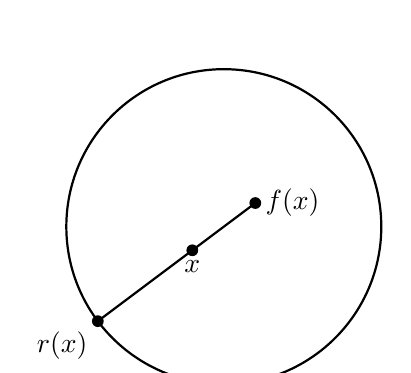
\begin{tikzpicture}[every path/.style={thick}]
      \draw circle [radius=2cm];
      \node[circ,inner sep=1.5pt] at (-0.4, -0.3) {};
      \node at (-0.4, -0.3) [below] {$x$};
      \node[circ,inner sep=1.5pt] at (0.4, 0.3) {};
      \node at (0.4, 0.3) [right] {$f(x)$};
      \draw (0.4, 0.3) -- (-1.6, -1.2);
      \node at (-1.6, -1.2) [circ,inner sep=1.5] {};
      \node at (-1.6, -1.2) [anchor = north east] {$r(x)$};
    \end{tikzpicture}
  \end{center}
  The map $r \colon \D^n \to \partial \D^n$ is continuous and
  $r\vert_{\partial \D^n} = \id$ so it is a retraction.
  Then by \Cref{cor:injective-i-surjective-r} the induced map
  $r_*$ must be surjective for all homology groups.
  In particular $r_* \colon H_{n-1}(\D^n) \to H_{n-1}(\partial \D^n) = H_{n-1}(S^{n-1})$
  must be surjective.
  However, we have already computed these homology groups,
  so we know that $r_*$ is a map from $\set{0}$ to $\Z$ so it can't be surjective.
  This contradiction completes the proof.
\end{proof}

\subsection{Relative homology}

\begin{definition}[Relative homology]
  Let $(X,A)$ be a pair such that $A \subseteq X$ where $X$ is a topological
  space.
  We have already seen that $C_n(A) \subseteq C_n(X)$.
  We define $C_n(X,A) := C_n(X) / C_n(A)$.
  This is the free abelian group with basis
  $\set{\sigma_{\alpha} \colon \Delta^n \to X}_{\alpha}$
  such that $\sigma_{\alpha}(\Delta^n) \nsubseteq A$.
  % direct complement?
\end{definition}
\begin{remark}
  Note that $\partial \colon C_n(X) \to C_{n-1}(X)$
  takes $\partial\del{C_n(A)} \subseteq C_{n-1}(A)$,
  and $\partial$ induces a map
  $\partial \colon C_n(X)/C_n(A) \to C_{n-1}(X)/C_{n-1}(A)$.
  This means that the boundary map
  $\partial \colon C_n(X,A) \to \colon C_{n-1}(X,A)$
  is well defined.
\end{remark}

\begin{remark}
  The pair $\del{C_n(X,A),\partial}$ is a chain complex because
  $\partial^2 = 0$.
\end{remark}

\begin{definition}[Relative homology]
  We define the homologies of $(X,A)$ (relative homology groups)
  to be the homologies of the chain complex $\del{C_n(X,A),\partial}$.
  We denote the relative homology groups with $H_n(X,A)$.
  This means that $H_n(X,A) = \ker \partial_n / \im \partial_{n+1}$
  for the boundary of the chain complex $\del{C_n(X,A),\partial}$.
\end{definition}

\begin{remark}
  A relative cycle is a relative chain $c + C_n(A) \in C_n(X,A)$
  for some $c \in C_n(X)$ such that $\partial(c) \in C_{n-1}(A)$.
  Below in red is an example of a relative $1$-cycle.
  \begin{center}
  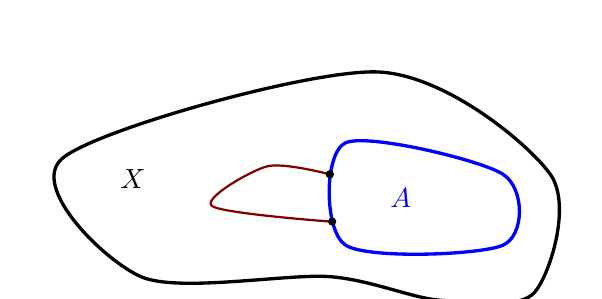
\begin{tikzpicture}
    \draw plot [smooth cycle] coordinates {(-2.4, -0.7) (0, -0.7) (1.4, -1) (2.6, -0.9) (2.8, 0.6) (0.6, 1.9) (-3.4, 0.8)};

    \draw[blue] plot [smooth cycle] coordinates {(0.2,1) (2.2,0.6) (2.2,-0.3) (0.2,-0.3)};
    \draw[thick, mred] plot [smooth] coordinates {(0,0) (-1.5, 0.2) (-0.8,0.7) (0,0.6)};
    \node [below] at (-2.5, 0.8) {$X$};
    \node [blue] at (0.9, 0.3) {$A$};
    \node [circ] at (0.03, 0) {};
    \node [circ] at (0, 0.6) {};
  \end{tikzpicture}
  \end{center}
\end{remark}

\begin{remark}
  A relative boundary is a relative chain $b + C_n(A) \in C_n(X,A)$
  for some $b \in C_n(X)$ such that
  $b + C_n(A) = \partial\del{c + C_{n+1}(A)} = \partial c + C_n(A)$
  for some $c + C_{n+1}(A) \in C_{n+1}(X,A)$.
  This is equialent to $b - \partial c \in C_n(A)$.
  Below in red is an example of a relative $2$-boundary.
  \begin{center}
  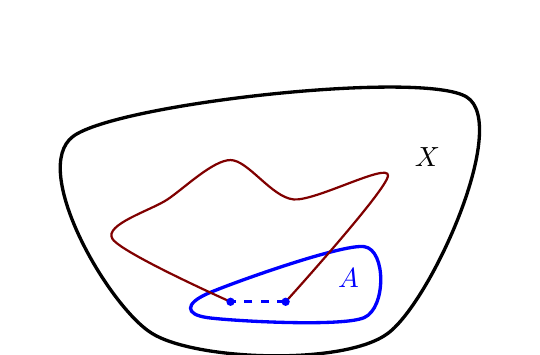
\begin{tikzpicture}
    \draw plot [smooth cycle] coordinates {(-2,1.5) (3,2) (2,-1) (-1,-1)};

    \draw[blue] plot [smooth cycle] coordinates {(-0.3,-0.5) (1.7,0.1) (1.7,-0.8) (-0.3,-0.8)};
    \draw[thick, mred] plot [smooth] coordinates {(0,-0.6) (-1.5, 0.2) (-0.8,0.7) (0,1.2) (0.8, 0.7) (2, 1) (0.7,-0.6)};
    \node[below] at (2.5, 1.5) {$X$};
    \node[blue] at (1.5, -0.3) {$A$};
    \node[circ,blue] at (0,-0.6) {};
    \node[circ,blue] at (0.7,-0.6) {};
    \draw[dashed,blue] (0.7,-0.6) -- (0,-0.6) {};
  \end{tikzpicture}
  \end{center}
\end{remark}

\begin{remark}
  The following red and green $1$-chains
  \begin{center}
    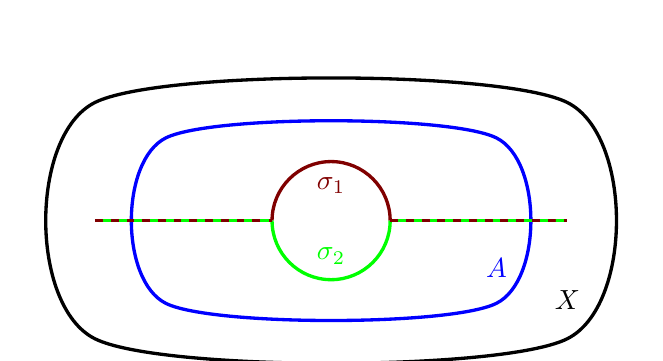
\begin{tikzpicture}[scale=1.5]
    \draw plot [smooth cycle] coordinates {(-2,1) (2,1) (2,-1) (-2,-1)};
    \draw[blue,scale=0.7] plot [smooth cycle] coordinates {(-2,1) (2,1) (2,-1) (-2,-1)};
    \draw[mred] (0:0.5) arc[start angle=0, end angle=180, radius=0.5];
    \draw[green] (180:0.5) arc[start angle=180, end angle=360, radius=0.5];
    \draw[
        mred,
        dash pattern=on 1mm off 1mm,
        postaction={draw, green, dash phase=1mm, dash pattern=on 1mm off 1mm}
    ] plot [smooth] coordinates {(-2,0) (-0.5,0)};
    \draw[
        mred,
        dash pattern=on 1mm off 1mm,
        postaction={draw, green, dash phase=1mm, dash pattern=on 1mm off 1mm}
    ] plot [smooth] coordinates {(0.5,0) (2.0,0)};
    \node[below] at (2, -0.5) {$X$};
    \node[blue] at (1.4, -0.4) {$A$};
    \node[mred] at (0, 0.3) {$\sigma_1$};
    \node[green] at (0, -0.3) {$\sigma_2$};
  \end{tikzpicture}
  \end{center}
  are not equal in $C_1(X,A)$.
  Recall that the sums of the singular chain groups are formal,
  this means that this is not a matter of pointwise function addition or anything,
  and certainly $\sigma_1 - \sigma_2$ is not an element of $C_n(A)$.
\end{remark}

\begin{definition}[Map of pairs]
  A map $f \colon (X,A) \to (Y,B)$ is said to be a map of pairs
  if it is continuous and $f(A) \subseteq B$.
\end{definition}
\begin{remark}
  A map of pairs $f$ induces a map on the relative homology groups.
  We denote it simply as $f_* \colon H_n(X,A) \to H_n(Y,B)$.
  Moreover, if $f,g \colon (X,A) \to (Y,B)$ and $f \simeq_{A} g$ then
  $f_* = g_*$.
  In order to show this we just notice that the prism operator $P$
  from \Cref{thm:homotopic-maps-induce-same-homomorphism-on-homology}
  takes $C_n(A)$ to $C_{n+1}(B)$,
  so it induces a relative prism operator $P \colon C_n(X,A) \to C_{n+1}(Y,B)$.
  Since the relative pris, operator is simply the prism operator
  reduced to quotient groups the formula
  $\partial P + P \partial = g_{\#} + f_{\#}$ is still satisfied,
  hence the maps $f_{\#}$ and $g_{\#}$ are homotopic on the relative chain
  groups, so they induce the same homomorphism on the relative homology groups.
\end{remark}

\begin{remark}
  The rows of the following diagram are short exact sequences
  \[\begin{tikzcd}
    0 & {C_n(A)} & {C_n(X)} & {C_n(X,A)} & 0 \\
    0 & {C_{n-1}(A)} & {C_{n-1}(X)} & {C_{n-1}(X,A)} & 0
    \arrow[from=1-1, to=1-2]
    \arrow["i_{\#}", from=1-2, to=1-3]
    \arrow["\partial"', from=1-2, to=2-2]
    \arrow["q_{\#}", from=1-3, to=1-4]
    \arrow["\partial"', from=1-3, to=2-3]
    \arrow[from=1-4, to=1-5]
    \arrow["\partial"', from=1-4, to=2-4]
    \arrow[from=2-1, to=2-2]
    \arrow["i_{\#}", from=2-2, to=2-3]
    \arrow["q_{\#}", from=2-3, to=2-4]
    \arrow[from=2-4, to=2-5]
  \end{tikzcd}\]
  and moreover, the diagram is commutative.
  This means that both $i_{\#}$ and $q_{\#}$ are chain maps.
  We can also keep adding rows to this diagram by considering more levels
  of chain groups.
  In this way, we get a short exact sequences of chain complexes
  \[\begin{tikzcd}
	0 & {\mathcal A} & {\mathcal B} & {\mathcal C} & 0
	\arrow[from=1-1, to=1-2]
	\arrow["i", from=1-2, to=1-3]
	\arrow["q", from=1-3, to=1-4]
	\arrow[from=1-4, to=1-5]
  \end{tikzcd}\]
  where $\mathcal A$ denotes the chain complexes of $A$,
  $\mathcal B$ denotes the chain complexes of $X$
  and $\mathcal C$ denotes the chain complexes of $(X,A)$.
\end{remark}

\begin{theorem}
  \label{thm:long-exact-consequence}
  Let
  \[\begin{tikzcd}
	0 & {\mathcal A} & {\mathcal B} & {\mathcal C} & 0
	\arrow[from=1-1, to=1-2]
	\arrow["i", from=1-2, to=1-3]
	\arrow["j", from=1-3, to=1-4]
	\arrow[from=1-4, to=1-5]
  \end{tikzcd}\]
  be a short exact sequence of chain complexes.
  Then there exists a long exact sequence (l.e.s) in homology
  \[\begin{tikzcd}
    \cdots & {H_n(\mathcal A)} & {H_n(\mathcal B)} & {H_n(\mathcal C)} & {H_{n-1}(\mathcal A)} & \cdots
    \arrow[from=1-1, to=1-2]
    \arrow["{i_*}", from=1-2, to=1-3]
    \arrow["{j_*}", from=1-3, to=1-4]
    \arrow["\partial", from=1-4, to=1-5]
    \arrow[from=1-5, to=1-6]
  \end{tikzcd}\]
\end{theorem}
\begin{remark}
  With regards to our previous example $i$ is the inclusion map
  and $j$ is the quotient map.
\end{remark}

\begin{corollary}
  If $(X,A)$ is a good pair, then the sequence
  \[\begin{tikzcd}
	\cdots & {H_n(A)} & {H_n(X)} & {H_n(X,A)} & {H_{n-1}(A)} & \cdots
	\arrow[from=1-1, to=1-2]
	\arrow["{i_*}", from=1-2, to=1-3]
	\arrow["{q_*}", from=1-3, to=1-4]
	\arrow["\partial", from=1-4, to=1-5]
	\arrow[from=1-5, to=1-6]
\end{tikzcd}\]
  is exact.
\end{corollary}

\begin{proofof}{\Cref{thm:long-exact-consequence}}
  The short exact sequence of chain complexes can be written as
  \[\begin{tikzcd}[ampersand replacement=\&,cramped]
    \& 0 \& 0 \& 0 \\
    \cdots \& {A_{n+1}} \& {A_n} \& {A_{n-1}} \& \cdots \\
    \cdots \& {B_{n+1}} \& {B_n} \& {B_{n-1}} \& \cdots \\
    \cdots \& {C_{n+1}} \& {C_n} \& {C_{n-1}} \& \cdots \\
    \& 0 \& 0 \& 0
    \arrow[from=1-2, to=2-2]
    \arrow[from=1-3, to=2-3]
    \arrow[from=1-4, to=2-4]
    \arrow[from=2-1, to=2-2]
    \arrow["\partial", from=2-2, to=2-3]
    \arrow["i", from=2-2, to=3-2]
    \arrow["\partial", from=2-3, to=2-4]
    \arrow["i", from=2-3, to=3-3]
    \arrow[from=2-4, to=2-5]
    \arrow["i", from=2-4, to=3-4]
    \arrow[from=3-1, to=3-2]
    \arrow["\partial", from=3-2, to=3-3]
    \arrow["j", from=3-2, to=4-2]
    \arrow["\partial", from=3-3, to=3-4]
    \arrow["j", from=3-3, to=4-3]
    \arrow[from=3-4, to=3-5]
    \arrow["j", from=3-4, to=4-4]
    \arrow[from=4-1, to=4-2]
    \arrow["\partial", from=4-2, to=4-3]
    \arrow[from=4-2, to=5-2]
    \arrow["\partial", from=4-3, to=4-4]
    \arrow[from=4-3, to=5-3]
    \arrow[from=4-4, to=4-5]
    \arrow[from=4-4, to=5-4]
  \end{tikzcd}\]
  Since $i$ and $j$ are chain maps, they commute with the boundary
  maps and thus this diagram commutes.
  In order to obtain the sequence
  \[\begin{tikzcd}
    \cdots & {H_n(\mathcal A)} & {H_n(\mathcal B)} & {H_n(\mathcal C)} & {H_{n-1}(\mathcal A)} & \cdots
    \arrow[from=1-1, to=1-2]
    \arrow["{i_*}", from=1-2, to=1-3]
    \arrow["{j_*}", from=1-3, to=1-4]
    \arrow["\partial", from=1-4, to=1-5]
    \arrow[from=1-5, to=1-6]
  \end{tikzcd}\]
  we need to have a map between $H_n(\mathcal C)$ and $H_{n-1}(\mathcal A)$.
  That's a map $\partial \colon C_n \to A_{n-1}$.
  Let $c \in C_n$.
  Since $j$ is surjective there exists $b \in B_n$ so that $j(b) = c$.
  We can then apply the boundary map on $b$ and send it to $B_{n-1}$.
  We now want to show that there exists $a \in A_{n-1}$ so that
  $i(a) = \partial(b)$, since this will allow us to map $c$ to that $a$.
  This means we need to show that $\partial(b) \in \im(i)$.
  By exactness we have $\im(i) = \ker(j)$ so we need to show that
  $j(\partial b) = 0$.
  Since $j$ commutes with $\partial$ we know that
  $j(\partial b) = \partial j(b) = \partial c$.
  This means that $\partial(b) \in \im(i)$
  if and only if $c \in \ker \partial_n$.
  This suffices to show the existence of a map between $H_n(\mathcal C)$
  and $H_{n-1}(\mathcal A)$.
  That is because $H_n(\mathcal C) = \ker \partial_n / \im \partial_{n+1}$
  so we only care about where we map elements of the kernel.
  We now have a map that maps $c \in H_n(\mathcal C)$ to some
  $a \in H_{n-1}(\mathcal A)$.
  We need to make sure that $a \in \ker \partial_{n-1}$ in order for the map
  to be well defined.
  Consider the diagram
   \[\begin{tikzcd}[ampersand replacement=\&,cramped]
    \& 0 \& 0 \& 0 \\
    \cdots \& {A_{n}} \& {A_{n-1}} \& {A_{n-2}} \& \cdots \\
    \cdots \& {B_{n}} \& {B_{n-1}} \& {B_{n-2}} \& \cdots
    \arrow[from=1-2, to=2-2]
    \arrow[from=1-3, to=2-3]
    \arrow[from=1-4, to=2-4]
    \arrow[from=2-1, to=2-2]
    \arrow["\partial", from=2-2, to=2-3]
    \arrow["i", from=2-2, to=3-2]
    \arrow["\partial", from=2-3, to=2-4]
    \arrow["i", from=2-3, to=3-3]
    \arrow[from=2-4, to=2-5]
    \arrow["i", from=2-4, to=3-4]
    \arrow[from=3-1, to=3-2]
    \arrow["\partial", from=3-2, to=3-3]
    \arrow["\partial", from=3-3, to=3-4]
    \arrow[from=3-4, to=3-5]
  \end{tikzcd}\]
  Since $a \in A_{n-1}$ we have $i(\partial a) \in B_{n-2}$.
  Since $i$ is a chain map $i(\partial a) = \partial i(a)$.
  We know from earlier that $i(a) = \partial b$ so we get that
  $i(\partial a) = \partial \partial b = 0$.
  This implies that $\partial a \in \ker(i)$, but since $i$ is injective
  $\partial a = 0$.
  More precisely $\partial_{n-1} a = 0$ so $a \in \ker \partial_{n-1}$
  so the map from $H_n(\mathcal C)$ to $H_{n-1}(\mathcal A)$ is well defined.
  It is left to show that the sequence
  \[\begin{tikzcd}
    \cdots & {H_n(\mathcal A)} & {H_n(\mathcal B)} & {H_n(\mathcal C)} & {H_{n-1}(\mathcal A)} & \cdots
    \arrow[from=1-1, to=1-2]
    \arrow["{i_*}", from=1-2, to=1-3]
    \arrow["{j_*}", from=1-3, to=1-4]
    \arrow["\partial", from=1-4, to=1-5]
    \arrow[from=1-5, to=1-6]
  \end{tikzcd}\]
  is exact.
  The arguemnts so far involved a lot of what's called \textit{diagram chasing}.
  I am sure I don't have to explain why that is.
  In order to complete the proof, we just show that the long sequence is exact,
  and we do this by definition.
  This means we do this by diagram chasing.
  Moreover, that diagram chasing is omitted from this proof.
\end{proofof}

\begin{remark}
  There is a version of \Cref{thm:long-exact-consequence} for reduced
  homology.
\end{remark}
\begin{example}
  Let $x \in X$.
  Then from \Cref{thm:long-exact-consequence} applied on $(X,\set{x})$
  we get that there exists a long exact sequence
  \[\begin{tikzcd}
    \cdots & {\widetilde H_n\del{\set{x}}} & {\widetilde H_n(X)} & {\widetilde H_n(X,x_0)} & {\widetilde H_{n-1}\del{\set{x}}} & \cdots
    \arrow[from=1-1, to=1-2]
    \arrow["{i_*}", from=1-2, to=1-3]
    \arrow["{q_*}", from=1-3, to=1-4]
    \arrow["\partial", from=1-4, to=1-5]
    \arrow[from=1-5, to=1-6]
  \end{tikzcd}\]
  and since we know that
  $\widetilde H_n\del{\set{x}} = \widetilde H_{n-1}\del{\set{x}} \cong \set{0}$
  and since this sequence is exact we get that
  $\widetilde H_n(X) \cong \widetilde H_n(X,x_0)$.
\end{example}

\begin{remark}[Long exact sequence of a triple]
  We can generalize the long exact sequence of a pair $(X,A)$ the a long
  exact sequence of a triple $(X,A,B)$, where $B \subset A \subset X$:
  \[\begin{tikzcd}[ampersand replacement=\&,cramped]
    \cdots \& {H_n(A,B)} \& {H_n(X,B)} \& {H_n(X,A)} \& {H_{n-1}(A,B)} \& \cdots
    \arrow[from=1-1, to=1-2]
    \arrow[from=1-2, to=1-3]
    \arrow[from=1-3, to=1-4]
    \arrow[from=1-4, to=1-5]
    \arrow[from=1-5, to=1-6]
  \end{tikzcd}\]
  This is just the long exact sequence of homology groups associated with
  the short exact sequence of chain complexes formed by the short exact
  sequences
  \[\begin{tikzcd}[ampersand replacement=\&,cramped]
    0 \& {C_{n}(A,B)} \& {C_{n}(X,B)} \& {C_{n}(X,A)} \& 0
    \arrow[from=1-1, to=1-2]
    \arrow[from=1-2, to=1-3]
    \arrow[from=1-3, to=1-4]
    \arrow[from=1-4, to=1-5]
  \end{tikzcd}\]
  For example, if $b$ is a point, the long exact sequence of the triple
  $(X,A,B)$ becomes the long exact sequence of reduced homology for the pair
  $(X,A)$.
\end{remark}

\subsection{Excisions}

\begin{theorem}[Excision]
  Let $Z \subseteq A \subseteq X$ so that $\overline Z \subseteq \mathring A$.
  Then the inclusion map $i \colon (X - Z, A - Z) \hookrightarrow (X,A)$
  induces an isomorphism $H_n(X,A) \cong H_n(X - Z, A - Z)$ for all $n$.
\end{theorem}
\begin{corollary}
  \label{cor:cor}
  Let $(X,A)$ be a good pair.
  Then $H_n(X,A) \simeq \widetilde H_n(X/A)$.
\end{corollary}
\begin{remark}
  An equivalent phrasing of the excision theorem is that if $X_1,X_2 \subseteq X$
  and $\mathring X_1 \cup \mathring X_2 = X$,
  then the inclusion $i \colon (X_1, X_1 \cap X_2) \hookrightarrow (X,X_2)$
  induces an isomorphism $H_n(X_1, X_1 \cap X_2) \cong H_n(X,X_2)$ for all $n$.
  In this case $A = X_2$ and $Z = X - X_1 = X_2 - X_1$ etc.
  Below are diagrams showing the equivalency of the theorems
  \[
    \tikz[eqpic,scale=0.8]{
      \draw plot [smooth cycle] coordinates {(-2,-2.5) (-2,2.5) (2,2.5) (2,-2.5)};
      \draw[orange,scale=0.95] plot [smooth cycle] coordinates {(-1.5,-2) (-1.5,2) (1.5,2) (1.5,-2)};
      \draw[blue,scale=0.8] plot [smooth cycle] coordinates {(-1,-1.5) (-1,1.5) (1,1.5) (1,-1.5)};
      \node[label=below:$\textcolor{blue}{Z}$]
        (cap) at (0,1.5) {};
      \node[label=center:$\textcolor{orange}{A}$]
        (cap) at (0,1.9) {};
    } \quad = \quad
    \tikz[eqpic]{
      \draw[morange] (2.5,1.5) -- (2.5,-1.5);
      \draw[mred] (-2.5,-1.5) -- (-2.5,1.5);
      
      \draw[mred] (-2.5,-1.5) -- (-1,-1.5);
      \draw[
          morange,
          dash pattern=on 1mm off 1mm,
          postaction={draw, mred, dash phase=1mm, dash pattern=on 1mm off 1mm}
      ] (-1,-1.5) -- (1,-1.5);
      \draw[morange] (1,-1.5) -- (2.5,-1.5);
      \draw[mred] (-2.5,1.5) -- (-1,1.5);
      \draw[
          morange,
          dash pattern=on 1mm off 1mm,
          postaction={draw, mred, dash phase=1mm, dash pattern=on 1mm off 1mm}
      ] (-1,1.5) -- (1,1.5);
      \draw[morange] (1,1.5) -- (2.5,1.5);

      \draw[morange] plot [smooth] coordinates
        {(-1,-1.5) (-1.25,-0.75) (-1.25,0.75) (-1,1.5)};
      \draw[mred] plot [smooth] coordinates
        {(1,-1.5) (1.25,-0.75) (1.25,0.75) (1,1.5)};
      \node[label=above:$\textcolor{mred}{X_1} \cap \textcolor{morange}{X_2}$]
        (cap) at (0,-1.5) {};
      \node[label=below:$\textcolor{mred}{X_1}$]
        (cap) at ({-3*2.5/4},1.5) {};
      \node[label=below:$\textcolor{morange}{X_2}$]
        (cap) at ({3*2.5/4},1.5) {};
    } \quad
    \begin{array}{l}
          A = X_2 \\
          Z = X - X_1 = X_2 - X_1 \\
          X - Z = X_1 \\
          A - Z = X_1 \cap X_2
    \end{array}
  \]
\end{remark}
\begin{definition}[$\U$-chains]
  Let $\U = \set{U_j}$ be a collection of subsets of $X$ such that their interiors
  form an open cover for $X$, that is, $X = \bigcup_{U \in \U} \mathring U$.
  Then we write
  \[
    C_n^{\U}(X) = \vspan\set{\sigma \colon \Delta^n \to X \mid 
    \exists U \in \U \st \sigma(\Delta^n) \subseteq U}.
  \]
\end{definition}
\begin{remark}
  Since $\partial (C_n^{U}(X)) \subseteq C_{n-1}^{U}(X)$,
  the groups $C_n^{\U}(X)$ form a chain complex.
  We denote the homology of this chain complex by $H_n^{\U}(X)$.
\end{remark}

\begin{proposition}
  The inclusion map $\iota \colon C_n^{\U}(X) \hookrightarrow C_n(X)$ is a homotopy equivalence
  between $C_n^{\U}(X)$ and $C_n(X)$.
  That is, there exists $\rho \colon C_n(X) \to C_n^{\U}(X)$,
  such that $\iota \circ \rho$ and $\rho \circ \iota$
  are chain homotopic to the identity.
  Hence $\iota$ induces isomorphisms $H_n^{\U}(X) \cong H_n(X)$ for all $n$.
\end{proposition}
\begin{proof}
  We will prove this proposition in four steps.
  \begin{enumerate}
    \item[(1)] \textit{Barycentric Subdivision of Simplicies}.
      Recall that any $n$-simplex given by $[v_0,v_1,\dots,v_n]$
      is defined to be all the points $\sum t_i v_i$ so that
      $t_i \geq 0$ and $\sum t_i = 1$.
      We define the barycenter\footnote{bary means mass} of an $n$-simplex to
      be the point with equal barycentric coordinates
      $b = \sum_{i=0}^{n} \frac{1}{n+1} v_i$.
      We define the barycenter subdivision of an $n$-simplex inductively.
      For $n = 0$ we define the subdivision as just the point itself
      \[
        BS\del{[v_0]} = \set{[v_0]}.
      \]
      We can now define the subdivision of a $n$-simplex 
      for $n = 1$ as follows:
      \[
        BS\del{[v_0,v_1]} =
        \bigcup_{i=0}^{1}
        \bigcup_{\scalebox{0.6}{$s\!\in\!BS\del{\Delta^i}$}} \set{[b,s]} =
        \set{[b,v_0], [b,v_1]},
      \]
      where $\Delta^i$ represents the $i$th face of the $\Delta$-complex,
      and $b$ is constant, it is the barycenter of the $1$-simplex.
      Inductively, we can assume that barycentric subdivision is defined
      for an $(n-1)$-simplex, and define
      \[
        BS\del{[v_0,v_1,\dots,v_n]} =
        \bigcup_{i=0}^{n}
        \bigcup_{\scalebox{0.6}{$s\!\in\!BS\del{\Delta^i}$}} \set{[b,s]}.
      \]
      Note that the barycentric division of an $n$-simplex
      is $(n+1)!$ $n$-simplices who cover the original $\Delta$-simplex.
      In particular $|BS([v_0,v_1,\dots,v_n])| = (n + 1)!$.
      Although this is not important for the proof, $BS(\Delta^n)$
      does form a simplicial complex structure on $\Delta^n$.
      We want to show that
      \[
        \diam[w_0,\dots,w_n] \le \frac{n}{n+1} \diam[v_0,\dots,v_n].
      \]
      for each $[w_0,\dots,w_n] \in BS(\Delta^n)$.
      We first observe that
      \[
        \diam[w_0,\dots,w_n] = \max\norm{w_i-w_j}
      \]
      becauase the distance of any two points $v$ and $\sum_i t_i v_i$
      always satisfies
      \[
        \abs{v - \sum_{i=0}^{n} t_i v_i} =
        \abs{\sum_{i=0}^{n} t_i (v - v_i)} \le
        \sum_{i=0}^{n} t_i |v - v_i| \le
        \sum_{i=0}^{n} t_i \max_j|v - v_j| =
        \max_j|v - v_j|.
      \]
      The rest of the proof is geometric.
      Its significance is that it allows us to divide any $n$-simplex
      into smaller simplicies with arbirarily small diameter.
    \item[(2)] The rest of the proof might be added eventually.
      % Hatcher 120-124(book) / 130-134(pdf)
    % \item[(2)] \textit{Barycentric Subdivision of Linear Chains}.
    %   Assume that $Y \subseteq \R^n$ is convex.
    %   Consider $LC_n(Y)$ to be the subspace of $C_n(Y)$ that is the span
    %   of all (affinely) linear simplices in $C_n(Y)$.
    %   This means that $\sigma \colon \Delta^n \to Y$ is given by
    %   $\sigma(\sigma_i t_i v_i) = \sum_i t_i \sigma(v_i)$,
    %   which are clearly determined by the images of $v_0,\dots,v_n$.
    %
    %   For all $b \in Y$ we define $b \colon LC_n(Y) \to LC_{n+1}(Y)$
    %   \[
    %     b\del{[w_0,\dots,w_n]} = [b,w_0,\dots,w_n].
    %   \]
    %   We have that
    %   \[
    %     \partial b(\sigma) =
    %     \partial b([w_0,\dots,w_n]) =
    %     \partial[b,w_0,\dots,w_n] =
    %     \sigma - b(\partial \sigma).
    %   \]
    %   We have that
    %   \[
    %     \partial b + b \partial = \id - 0
    %   \]
    %   ($b$ is a chain homotopy between the identity and the zero map).
    %   % from the chain to itself
    %   % recall that a chain homotopy is a map p such that
    %   % \partial p + p \partial = f - g
    %   % p increases the dimension
    %   Define $S \colon LC_n(Y) \to LC_n(Y)$
    %   inductively by $S\del{[\emptyset]} = [\emptyset]$.
    %
    %   If $\lambda$ is a simplex,
    %   denote by $b_{\lambda}$ its barycenter.
    %   Define
    %   \[
    %     S(\lambda) = b_{\lambda}(S \partial \lambda).
    %   \]
    %   So $S$ is a chain map $(\partial S = S \partial)$.
    %   \[
    %     \partial S(\sigma) = \partial b_{\sigma}(S \partial \sigma),
    %   \]
    %   and we have seen that $\partial b(\sigma) = \sigma - b(\partial \sigma)$ so
    %   \[
    %     \partial S(\sigma) =
    %     S \partial (\sigma) - b_{\sigma}(\partial S \partial \sigma) = % induction hypothesis
    %     S \partial (\sigma) - 
    %       b_{\sigma}(S \underbrace{\partial \partial \sigma}_{=\,0}) =
    %       S \partial (\sigma).
    %   \]
    %   % reality check, we can only commute S with the left \partial (or right 5050)
    %   Define $T \colon LC_n(Y) \to LC_{n+1}(Y)$ inductively by
    %   \[
    %     T(\sigma) = b_{\sigma}\del{\sigma - T \partial \sigma}.
    %   \]
    %   % prism operator???
    %   We want to show that $\partial T + T \partial = \id - S$.
    %   We have that
    %   \begin{align*}
    %     \partial T(\sigma) &=
    %     \partial b_{\sigma}\del{\sigma - T \partial \sigma} \\ &=
    %     (\sigma - T \partial \sigma) - 
    %     b_{\sigma}\del{\partial \sigma - \partial T \partial \sigma} \\ &=
    %     (\sigma - T \partial \sigma) - 
    %     b_{\sigma}\del{\partial \sigma - 
    %   \partial \del{\sigma - S \sigma - \partial T \sigma}} \\ &=
    %     (\sigma - T \partial \sigma) - 
    %   \underbrace{b_{\sigma}\del{\partial S \sigma}}_{S \sigma} \\ &=
    %   \sigma - S \sigma - T \partial \sigma \\ &=
    %     (\id - S - T \partial) \sigma
    %   \end{align*}
    %   % T is a chain homotopy
    % \item[(3)]
%       We have shown that there exists $\iota \colon C^U_n(X) \to C_n(X)$
% which induces an isomorphism in homology $\iota_* \colon H^U_n(X) \to H_n(X)$.
%
% We want to show that there exists a map going the other way
% $\rho \colon C_n(X) \to C^U_n(X)$ such that $\rho i$ and $i \rho$
% are chain homotopic to $\id_{C_n}$ and $\id_{C_n^U}$.
  \end{enumerate}
\end{proof}

\begin{theorem}[Excision]
  Let $X$ be a topological space so that $A,B \subseteq X$
  and $\mathring A \cup \mathring B = X$.
  Then the inclusion map $i \colon (B,A \cap B) \hookrightarrow (X,A)$
  induces an isomorphism $H_n(B, A \cap B) \cong H_n(X,A)$.
\end{theorem}
\begin{proof}
  dependent on proof of excision. to be added.
  % By definition we have that $C_n(X,A) = C_n(X)/C_n(A)$.
  % Let $\U = \set{A,B}$.
  % We have seen earlier that
  % \[
  %   C_n(X) \longleftrightarrow_{\iota,\rho} C_{n}^{\U}(X).
  % \]
  % We have that $\iota$, $\rho$ and $D$ send $C_n(A) \to C_n(A)$
  % \[
  %   \implies
  %   C_n(X)/C_n(A) \longleftrightarrow_{\iota,\rho} C_{n}^{\U}(X)/C_n(A)
  %   \simeq C_n(B) / C_n(A \cap B).
  % \]
  % We then get that their homology is equal
  % \[
  %   H_n(X,A) \simeq H_n(B,A \cap B).
  % \]
\end{proof}

% add remark with content in a picture on phone | probabaly l.e.s of triple & the following theorem

\begin{theorem}
  \label{thm:reduced-and-relative-homologies}
  Let $(X,A)$ be a good pair.
  Then the quotient map $q \colon (X,A) \to (X/A,A/A)$ induces an
  isomorphism $q_* \colon H_n(X,A) \to H_n(X/A,A/A) \cong \widetilde H_n(X/A)$
  for all $n$.
\end{theorem}
\begin{proof}
  We have seen that a space relative to a point is isomorphic
  to the reduced homology of the space.
  Therefore we only need to show an isomorphism
  $q_* \colon H_n(X,A) \to H_n(X/A,A/A)$.
  Let $U$ be a neighbourhood of $A$ in $X$ that deformation retracts onto $A$.
  We have the commutative diagram
  \[\begin{tikzcd}[ampersand replacement=\&,cramped]
    {H_n(X,A)} \& {H_n(X,U)} \& {H_n(X-A,U-A)} \\
    {H_n(X/A,A/A)} \& {H_n(X/A,U/A)} \& {H_n(X/A-A/A,U/A-A/A)}
    \arrow[from=1-1, to=1-2]
    \arrow["{q_*}", from=1-1, to=2-1]
    \arrow["{q_*}", from=1-2, to=2-2]
    \arrow[from=1-3, to=1-2]
    \arrow["{q_*}", from=1-3, to=2-3]
    \arrow[from=2-1, to=2-2]
    \arrow[from=2-3, to=2-2]
  \end{tikzcd}\]
  In the long exact sequence of the triple $(X,U,A)$ we get that
  \[\begin{tikzcd}[ampersand replacement=\&,cramped]
    \cdots \& {H_n(U,A)} \& {H_n(X,A)} \& {H_n(X,U)} \& {H_{n-1}(U,A)} \& \cdots
    \arrow[from=1-1, to=1-2]
    \arrow[from=1-2, to=1-3]
    \arrow[from=1-3, to=1-4]
    \arrow[from=1-4, to=1-5]
    \arrow[from=1-5, to=1-6]
  \end{tikzcd}\]
  and since a deformation retraction of $U$ onto $A$ gives a homotopy
  equivalence of pairs $(U,A) \simeq (A,A)$ we have that
  $H_n(U,A) \cong H_n(A,A)$ for all $n$,
  so $H_n(U,A) \cong H_n(U,A) \cong \set{0}$ and thus
  from the exactness of the sequence $H_n(X,A) \cong H_n(X,U)$
  so we may assume the upper left horizontal arrow in our commutative diagram
  is an isomorphism.
  The deformation retraction from $U$ to $A$ induces a deformation
  retraction of $U/A$ onto $A/A$, so the same argument shows that we may
  assume the lower left horizontal arrow in our commutative diagram
  is an isomorphism as well.
  The other two horizontal maps are isomorphisms directly from excision.
  The right vertical map $q_*$ is an isomorphism since we can see by recalling
  point set topology that $q$ restricts
  to a homeomorphism on the complement of $A$.
  From the commutativity of the diagram it follows that the middle $q_*$
  and then also the left $q_*$ is an isomorphism.
\end{proof}

% maybe include X \cup CA thing for general pairs.

\begin{theorem}
  \label{thm:invariance-of-dimension}
  Let $U \subseteq \R^n$ and $V \subseteq \R^m$ be homeomorphic open sets.
  Then $m = n$.
\end{theorem}
\begin{proof}
  We want to compute the local homology at $x \in U$
  \[
    H_k(X, X - \set{x}).
  \]
  From the excision theorem we have that
  \[
    \widetilde H_k(U, U - \set{x}) \cong
    \widetilde H_k(\R^n, \R^n - \set{x}).
  \]
  We consider the long exact sequence of $\R^n - \set{x} = A \subset X = \R^n$,
  \[\begin{tikzcd}
    {\widetilde H_k(\R^n)} & {\widetilde H_k(\R^n,\R^n-\set{x})} & {\widetilde H_{k-1}(\R^n-\set{x})} & {\widetilde H_{k-1}(\R^n)}
    \arrow[from=1-1, to=1-2]
    \arrow[from=1-2, to=1-3]
    \arrow[from=1-3, to=1-4]
  \end{tikzcd}.\]
  We know that $\widetilde H_k(\R^n) = \widetilde H_{k-1}(\R^n) = \set{0}$
  which implies that
  $\widetilde H_k(\R^n,\R^n-\set{x}) \cong \widetilde H_{k-1}(\R^n-\set{x})$.
  Moreover, we can now combine the result that
  $\widetilde H_{k-1}(\R^n-\set{x}) \cong \widetilde H_{k-1}(S^{n-1})$
  and the result from the excision theorem to get
  \[
    \widetilde H_k(U, U - \set{x}) \cong
    \widetilde H_k(\R^n,\R^n-\set{x}) \cong
    \widetilde H_{k-1}(S^{n-1}) =
    \begin{cases}
      \Z, &k = n, \\
      \set{0}, &\text{otherwise}.
    \end{cases}
  \]
  Let $\varphi \colon U \to V$ be a homeomorphism.
  By $\varphi_*$
  we get $\widetilde H_k(U,U-\set{x}) \cong H_k(V,V-\set{\varphi(x)})$.
  We can repeat the same process from earlier and get that
  \[
    \widetilde H_k(V, V - \set{\varphi(x)}) \cong
    \widetilde H_{k-1}(S^{m-1}) =
    \begin{cases}
      \Z, &k = m, \\
      \set{0}, &\text{otherwise},
    \end{cases}
  \]
  which implies that $n = m$.
\end{proof}
\begin{remark}
  The result of \Cref{thm:invariance-of-dimension}
  is also sometimes referred to as ``invariance of dimension''.
\end{remark}
\begin{remark}
  In the proof of \Cref{thm:invariance-of-dimension}
  we have seen the concept of \textit{local homology}.
  That is, the homology group $H_n(X, X - \set{x})$.
  The reason this is called local homology, is because as long as we assume
  $\set{x}$ is closed,
  we get from excision that $H_n(X, X - \set{x}) \cong H_n(U, U - \set{x})$.
  This shows that the structure of this group depends only on the local
  topology of $X$ around $x$.
  Since a homeomorphism must induce isomorphisms
  $H_n(X, X - \set{x}) \cong H_n(Y, Y - \set{f(x)})$
  for all $x$ and all $n$, the local homology groups can be used to
  tell when spaces are not locally homeomorphic at certain points,
  as in \Cref{thm:invariance-of-dimension}.
\end{remark}

\begin{remark}
  We have seen that
  \[
    H_k(\D^n,\partial \D^n) \cong
    \widetilde H_k(S^n) =
    \begin{cases}
      \Z, &n = k, \\
      \set{0},  &\text{otherwise}.
    \end{cases}
  \]
  In the following proposition we will find the explicit cycle
  that generates $H_n(S^n) \cong H_n(\D^n,\partial \D^n)$
  where we identify
  $H_n(\D^n,\partial \D^n) \cong H_n(\Delta^n,\partial \Delta^n)$.
\end{remark}

\begin{proposition}
  The map $\sigma_n \colon \Delta^n \to \Delta^n$
  where $\sigma_n = \id_n$ viewed as a singular $n$-simplex is the generator of
  $H_n(\Delta^n,\partial \Delta^n) \cong \Z$.
\end{proposition}
\begin{proof}
  Note that since $\partial \sigma_n \in C_{n-1}(\partial \Delta^n)$
  we have
  $\partial \sigma_n = 0 \in C_{n-1}(\Delta^n) / C_{n-1}(\partial \Delta^n)$
  and thus $\sigma_n$ is a cycle so
  $[\sigma_n] \in H_n(\Delta^n, \partial \Delta^n)$.
  We will prove the proposition by induction on $n$.

  When $n = 0$ then $\sigma$ is clearly the generator of
  $H_0(\Delta^0 / \partial \Delta^0) = H_0(\set{*} / \emptyset) = H_0(\set{*})$.

  When $n > 0$ let $\Lambda = \partial \Delta^n - \mathring \Delta_i$
  where $\Delta_i$ is some face of $\Delta^n$
  (please appreciate the incredible notation).
  We claim that there exist isomorphisms
  \[\begin{tikzcd}[ampersand replacement=\&,cramped]
    {H_n(\Delta^n,\partial \Delta^n)} \& {H_{n-1}(\partial \Delta^n, \Lambda)} \& {H_{n-1}(\Delta^{n-1},\partial \Delta^{n-1})}
    \arrow["\cong", from=1-1, to=1-2]
    \arrow["\cong"', from=1-3, to=1-2]
  \end{tikzcd}\]
  Consider the long exact sequence of the triple
  $(\Delta^n, \partial \Delta^n, \Lambda)$
  \[\begin{tikzcd}[ampersand replacement=\&,cramped]
    \cdots \& {H_n(\partial \Delta^n,\Lambda)} \& {H_n(\Delta^n,\Lambda)} \& {H_n(\Delta^n,\partial \Delta^n)} \& {H_{n-1}(\partial \Delta^n,\Lambda)} \& \cdots
    \arrow[from=1-1, to=1-2]
    \arrow[from=1-2, to=1-3]
    \arrow[from=1-3, to=1-4]
    \arrow[from=1-4, to=1-5]
    \arrow[from=1-5, to=1-6]
  \end{tikzcd}\]
  We know that elements of the form $H_i(\Delta^n,\Lambda)$ are the zero group
  since $\Delta^n$ deformation retracts onto $\Lambda$,
  so $(\Delta^n,\Lambda) \simeq (\Lambda,\Lambda)$ and $H_i(\Delta^n,\Lambda)$
  is trivial.
  By exactness of the long exact sequence we get the first isomorphism
  $H_n(\Delta^n,\partial \Delta^n) \cong H_{n-1}(\partial \Delta^n, \Lambda)$.

  The second isomorphism is induced by the inclusion
  $i \colon \Delta^{n-1} \hookrightarrow \partial \Delta^n$
  as the face not contained in $\Lambda$.
  When $n = 1$, the inclusion clearly induces an isomorphism
  between $H_0(\Delta^0, \partial \Delta^0)$
  and $H_0(\partial \Delta^n, \Lambda)$.
  When $n > 1$, the set $\partial \Delta^{n-1}$ is nonempty so both
  $(\partial \Delta^n, \Lambda)$ and $(\Delta^{n-1},\partial \Delta^{n-1})$
  are good pairs.
  Then $i$ induces a homeomorphism of the quotients
  $\partial \Delta^n / \Lambda \cong \Delta^{n-1} / \partial \Delta^{n-1}$.
  This shows the existence of the second isomorphism.

  We get that $[\sigma]$ is sent (under the first isomorphism)
  to $[\partial \sigma] = \pm [\sigma_{n-1}]$
  where $\sigma_{n-1}$ is the identity on one of the faces of $\Delta^n$.

  By the inductive hypothesis $\sigma_{n-1}$ is a generator
  of $H_{n-1}(\Delta^{n-1}, \partial \Delta^{n-1})$
  so $\partial \sigma_n$ is a generator of $H_n(\partial \Delta^n, \Lambda)$
  and hence $\sigma_n$ is a generator of $H_n(\Delta^n, \partial \Delta^n)$
  (because they are images of each other through the isomorphisms).

  In order to describe the cycle generating $\widetilde H_n(S^n)$
  (this is very similar to a problem from the homework)
  we first identify
  $S^n \cong \Delta^n_1 \cup \Delta^n_2 / \partial \Delta^n_1 \sim \partial \Delta^n_2$
  so that the boundaries are glued in the obvious way (the one that preserves
  the order of the vertices).
  Let $\sigma_{1,2}$ be the singular $n$-simplices that
  represent $\Delta^n_{1,2}$.
  We claim that $[\sigma_1 - \sigma_2]$ is the generator of $\widetilde H_n(S^n)$.

  We have that $[\sigma_1 - \sigma_2] \in \widetilde H_n(S^n)$.
  Consider the isomorphisms
  \[\begin{tikzcd}
    {\widetilde H_n(S^n)} & {\widetilde H_n(S^n,\Delta^n_2)} & {\widetilde H_n(\Delta^n_1,\partial \Delta^n_1)}
    \arrow["\cong", from=1-1, to=1-2]
    \arrow["\cong"', from=1-3, to=1-2]
  \end{tikzcd}\]
  The first isomorphism comes from the long exact sequence of the pair
  $(S^n, \Delta_2^n)$ and the second isomorphism is justified in the
  nontrivial cases $n > 0$ by passing to quotients as before.
  Under these isomorphisms the cycle $\sigma_1 - \sigma_2$ in the first
  group corresponds to the cycle $\Delta_1^n$ in the third group,
  which represents a generator of this group as we have seen,
  so $\Delta_1^n - \Delta_2^n$ represents a generator of $\widetilde H_n(S^n)$.
\end{proof}

\begin{proposition}
  Let $\set{(X_{\alpha},x_{\alpha})}_{\alpha}$ be a collection of good pairs.
  Then the inclusion maps
  $i_{\alpha} \colon X_{\alpha} \hookrightarrow \bigvee_{\alpha} X_{\alpha}$
  induce an isomorphism
  \[
    \bigoplus_{\alpha} (i_{\alpha})_* \colon
    \widetilde H_k\del{\bigvee_{\alpha} (X_{\alpha},x_{\alpha})} \taking{\cong}
    \bigoplus_{\alpha} \widetilde H_k(X_{\alpha}).
  \]
\end{proposition}
\begin{proof}
  Notice that the pair $(\bigsqcup X_{\alpha}, \set{x_{\alpha} \mid \alpha})$
  is a good pair.
  Since reduced homology is the same as homology relative to a basepoint,
  the result follows from \Cref{thm:reduced-and-relative-homologies}
  by taking $(X,A) = (\bigsqcup X_{\alpha}, \set{x_{\alpha} \mid \alpha})$.
  Then
  \begin{align*}
  \widetilde H_k\del{\bigsqcup_{\alpha} X_{\alpha} / \set{x_{\alpha} \mid \alpha}}
      &\cong H_k\del{\bigsqcup_{\alpha} X_{\alpha}, \set{x_{\alpha}}_{\alpha}} \\
      &= \bigoplus_{\alpha} H_k(X_{\alpha},x_{\alpha}) \\
      &= \bigoplus_{\alpha} \widetilde H_k(X_{\alpha}).
  \end{align*}
\end{proof}

\subsection{Mayer--Vietoris}
\begin{theorem}
  Let $X = \mathring A \cup \mathring B$ where $A,B \subseteq X$.
  Consider the following diagram:
  \begin{center}
  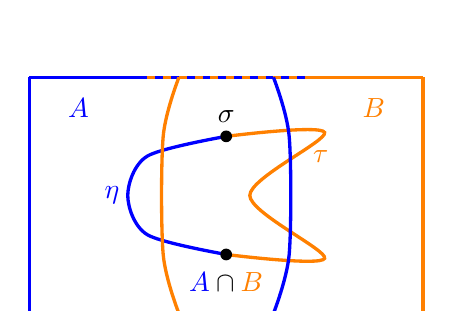
\begin{tikzpicture}
    \draw[blue] plot [smooth] coordinates {(0,-1.5+0.75) (-1,-0.5) (-1.25,0) (-1,0.5) (0,0.75)};
    \draw[morange] plot [smooth] coordinates {(0,0.75) (1.25,0.8) (0.3,0) (1.25,-0.8) (0,-1.5+0.75)};
    \node[circle,fill,inner sep=1.5pt] (pt1) at (0,0.75) {};
    \node[circle,fill,inner sep=1.5pt] (pt2) at (0,-0.75) {};
    \node[inner sep=1.5pt,label=center:$\sigma$] (sigma) at (0,1) {};
    \node[inner sep=1.5pt,label=center:$\textcolor{morange}{\tau}$] (tau) at (1.2,0.5) {};
    \node[inner sep=1.5pt,label=center:$\textcolor{blue}{\eta}$] (eta) at (-1.45,0) {};
    \draw[morange] (2.5,1.5) -- (2.5,-1.5);
      \draw[blue] (-2.5,-1.5) -- (-2.5,1.5);
      
      \draw[blue] (-2.5,-1.5) -- (-1,-1.5);
      \draw[
          morange,
          dash pattern=on 1mm off 1mm,
          postaction={draw, blue, dash phase=1mm, dash pattern=on 1mm off 1mm}
      ] (-1,-1.5) -- (1,-1.5);
      \draw[morange] (1,-1.5) -- (2.5,-1.5);
      \draw[blue] (-2.5,1.5) -- (-1,1.5);
      \draw[
          morange,
          dash pattern=on 1mm off 1mm,
          postaction={draw, blue, dash phase=1mm, dash pattern=on 1mm off 1mm}
      ] (-1,1.5) -- (1,1.5);
      \draw[morange] (1,1.5) -- (2.5,1.5);

      \draw[morange] plot [smooth] coordinates
        {(-0.6,-1.5) (-0.8,-0.75) (-0.8,0.75) (-0.6,1.5)};
      \draw[blue] plot [smooth] coordinates
        {(0.6,-1.5) (0.8,-0.75) (0.8,0.75) (0.6,1.5)};
      \node[label=above:$\textcolor{blue}{A} \cap \textcolor{morange}{B}$]
        (cap) at (0,-1.5) {};
      \node[label=below:$\textcolor{blue}{A}$]
        (cap) at ({-3*2.5/4},1.5) {};
      \node[label=below:$\textcolor{morange}{B}$]
        (cap) at ({3*2.5/4},1.5) {};
  \end{tikzpicture}
  \end{center}
  Then
  \[\begin{tikzcd}[ampersand replacement=\&,cramped]
    \&\& {([\tau],[\eta])} \& {[\tau]+[\eta]} \\
    \cdots \& {H_n(A \cap B)} \& {H_n(A) \oplus H_n(B)} \& {H_n(X)} \& {H_{n-1}(A \cap B)} \& \cdots \\
    \& {[\sigma]} \& {([\sigma],-[\sigma])} \& {[\sigma]=[\tau]+[\eta]} \& {\partial \tau}
    \arrow[maps to, from=1-3, to=1-4]
    \arrow[from=2-1, to=2-2]
    \arrow[from=2-2, to=2-3]
    \arrow[from=2-3, to=2-4]
    \arrow[from=2-4, to=2-5]
    \arrow[from=2-5, to=2-6]
    \arrow[maps to, from=3-2, to=3-3]
    \arrow[from=3-4, to=3-5]
  \end{tikzcd}\]
  is a long exact sequence.
\end{theorem}
\begin{proof}
  Let $\U = \set{A,B}$.
  The sequence
  \[\begin{tikzcd}[ampersand replacement=\&,cramped]
    0 \& {C_n(A \cap B)} \& {C_n(A) \oplus C_n(B)} \& {C_n^{\U}(X)} \& 0
    \arrow[from=1-1, to=1-2]
    \arrow["f",from=1-2, to=1-3]
    \arrow["g",from=1-3, to=1-4]
    \arrow[from=1-4, to=1-5]
  \end{tikzcd}\]
  where $f \colon \sigma \mapsto (\sigma,-\sigma)$
  and $g \colon (\sigma,\eta) \mapsto \sigma + \eta$ is 
  a short exact sequence of chains.
  Since $H_n(X) \cong H_n^{\U}(X)$ and this is a short exact sequence,
  the long exact sequence in homology is the result,
  which concludes the proof.
\end{proof}
\begin{remark}
  We can do the same with exact sequences of reduced homology.
\end{remark}

\begin{example}
  We want to find $\widetilde H_k(S^n)$.
  Let $S^n = \mathring A \cup \mathring B$
  where $A = S^n - \set{N}$ and $B = S^n - \set{S}$
  where $\set{S,N}$ are the south and north poles of the $n$-sphere.

  We know that $A \cong B \cong \R^n$ so they are both contractible.
  We also see that $A \cap B \simeq_{\dr} S^{n-1}$
  since there exists a deformation retraction from $A \cap B$
  to the equator, which is $S^{n-1}$.

  By the Mayer--Vietoris theorem we get that
  \[\begin{tikzcd}[ampersand replacement=\&,cramped]
    {\widetilde H_k(A) \oplus \widetilde H_k(B)} \& {\widetilde H_k(S^n)} \& {\widetilde H_{k-1}(A \cap B)} \& {\widetilde H_{k-1}(A) \oplus \widetilde H_{k-1}(B)}
    \arrow[from=1-1, to=1-2]
    \arrow[from=1-2, to=1-3]
    \arrow[from=1-3, to=1-4]
  \end{tikzcd}\]
  and by our calculations this is equal to
  \[\begin{tikzcd}[ampersand replacement=\&,cramped]
    {\set{0} \oplus \set{0}} \& {\widetilde H_k(S^n)} \& {\widetilde H_{k-1}(S^{n-1})} \& {\set{0} \oplus \set{0}}
    \arrow[from=1-1, to=1-2]
    \arrow[from=1-2, to=1-3]
    \arrow[from=1-3, to=1-4]
  \end{tikzcd}\]
  so $H_k(S^n) \cong H_{k-1}(S^{n-1})$.
  This allows us to compute the homologies of the sphere inductively
  like we have done in \Cref{cor:homologies-of-spheres}.
\end{example}

\begin{example}
  Consider the space $\RP^2$.
  We can choose $A \cong \D^2$ and $B \cong M$ where $M$ is the M\"obius
  band.
  \begin{center}
    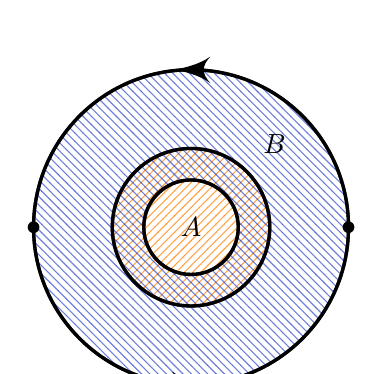
\begin{tikzpicture}[scale=2]
      \draw[pattern=north east lines,opacity=0.7,pattern color=orange]
        (0,0) circle (0.5cm) {};
      \draw[pattern=north west lines, opacity=0.7, pattern color=mblue, even odd rule]
    (0,0) circle (1cm)  % Outer circle
    (0,0) circle (0.3cm);    % Inner circle (subtracted)
      \draw (0:0.5) arc[start angle=0, end angle=360, radius=0.5];
      \draw (0:0.3) arc[start angle=0, end angle=360, radius=0.3];
      \draw[-->]
        (90:1) arc[start angle=90, end angle=270, radius=1];
      \draw[-->]
        (-90:1) arc[start angle=-90, end angle=90, radius=1];
      \node[fill, circle, inner sep=1.5pt] (v0) at (180:1) {};
      \node[fill, circle, inner sep=1.5pt] (v1) at (0:1) {};
      \node[inner sep=1.5pt, label=center:$A$] (A) at (0:0) {};
      \node[inner sep=1.5pt, label=center:$B$] (A) at (45:0.75) {};
    \end{tikzpicture}
  \end{center}
  Then from Mayer--Vietoris we get the following long exact sequence:
  \[
  \begin{tikzcd}
    \cdots \ar[r] & \widetilde H_2(A) \oplus \widetilde H_2(B) \ar[r] & \widetilde H_2(\RP^2) \ar[r] & \widetilde H_1(A \cap B) \ar[out=0, in=180, looseness=2, overlay, lld]\\
    & \widetilde H_1(A) \oplus \widetilde H_1(B) \ar[r] & \widetilde H_1(\RP^2) \ar[r] & \widetilde H_0(A \cap B) \ar [r] & \cdots
  \end{tikzcd}
  \]
  We know that $A$ is contractible
  so $\widetilde H_{1}(A) = \widetilde H_{2}(A) = \set{0}$
  and the M\"obius band has a deformation retraction to $S^1$.
  So does $A \cap B$.
  We now have an exact sequence of the form
  \[\begin{tikzcd}[ampersand replacement=\&,cramped]
    0 \& {\widetilde H_2(\RP^2)} \& \Z \& \Z \& {\widetilde H_1(\RP^2)} \& 0
    \arrow[from=1-1, to=1-2]
    \arrow[from=1-2, to=1-3]
    \arrow[from=1-3, to=1-4]
    \arrow[from=1-4, to=1-5]
    \arrow[from=1-5, to=1-6]
  \end{tikzcd}\]
  Since we know what the maps in the Mayer--Vietoris sequence
  are, we can see that the generator of the left $\Z$
  is sent to twice the generator of the right $\Z$.
  This means that $\widetilde H_2(\RP^2) = 0$ and
  that $\widetilde H_1(\RP^2) = \Z/2\Z$.
  % give intuition to Z/2Z
  % explain??
  \[\begin{tikzcd}[ampersand replacement=\&,cramped]
    0 \& 0 \& \Z \& \Z \& {\Z/2\Z} \& 0
    \arrow[from=1-1, to=1-2]
    \arrow[from=1-2, to=1-3]
    \arrow[from=1-3, to=1-4]
    \arrow[from=1-4, to=1-5]
    \arrow[from=1-5, to=1-6]
  \end{tikzcd}\]
\end{example}

\subsection{Naturality}
\begin{remark}
  The etymology of ``naturality'' will come after we understand
  its categorical interpretation.
\end{remark}

\begin{definition}[Naturality]
  To say that he long exact sequence of a pair is \textit{natural}
  means that for a map $f \colon (X,A) \to (Y,B)$,
  the diagram
  \[\begin{tikzcd}[ampersand replacement=\&,cramped]
    \cdots \& {H_n(A)} \& {H_n(X)} \& {H_n(X,A)} \& {H_{n-1}(A)} \& \cdots \\
    \cdots \& {H_n(B)} \& {H_n(Y)} \& {H_n(Y,B)} \& {H_{n-1}(B)} \& \cdots
    \arrow[from=1-1, to=1-2]
    \arrow["{i_*}", from=1-2, to=1-3]
    \arrow["{f_*}", from=1-2, to=2-2]
    \arrow["{q_*}", from=1-3, to=1-4]
    \arrow["{f_*}", from=1-3, to=2-3]
    \arrow["\partial", from=1-4, to=1-5]
    \arrow["{f_*}", from=1-4, to=2-4]
    \arrow[from=1-5, to=1-6]
    \arrow["{f_*}", from=1-5, to=2-5]
    \arrow[from=2-1, to=2-2]
    \arrow["{i_*}", from=2-2, to=2-3]
    \arrow["{q_*}", from=2-3, to=2-4]
    \arrow["\partial", from=2-4, to=2-5]
    \arrow[from=2-5, to=2-6]
  \end{tikzcd}\]
  commutes.
\end{definition}

\begin{remark}
  There is also a more general algebraic fact that the long exact
  sequence of homology groups associated with a short exact sequence of
  chain complexes is natural.
  This means that that diagram
  \[\begin{tikzcd}[ampersand replacement=\&,cramped]
    \cdots \& {H_n(\mathcal A)} \& {H_n(\mathcal B)} \& {H_n(\mathcal C)} \& {H_{n-1}(\mathcal A)} \& \cdots \\
    \cdots \& {H_n(\mathcal A')} \& {H_n(\mathcal B')} \& {H_n(\mathcal C')} \& {H_{n-1}(\mathcal A')} \& \cdots
    \arrow[from=1-1, to=1-2]
    \arrow["{i_*}", from=1-2, to=1-3]
    \arrow["{\alpha_*}", from=1-2, to=2-2]
    \arrow["{q_*}", from=1-3, to=1-4]
    \arrow["{\beta_*}", from=1-3, to=2-3]
    \arrow["\partial", from=1-4, to=1-5]
    \arrow["{\gamma_*}", from=1-4, to=2-4]
    \arrow[from=1-5, to=1-6]
    \arrow["{\alpha_*}", from=1-5, to=2-5]
    \arrow[from=2-1, to=2-2]
    \arrow["{i'_*}", from=2-2, to=2-3]
    \arrow["{q'_*}", from=2-3, to=2-4]
    \arrow["\partial", from=2-4, to=2-5]
    \arrow[from=2-5, to=2-6]
  \end{tikzcd}\]
  commutes.
% % https://q.uiver.app/#q=WzAsMTAsWzAsMCwiMCJdLFsxLDAsIlxcbWF0aGNhbCBBIl0sWzIsMCwiXFxtYXRoY2FsIEIiXSxbMywwLCJcXG1hdGhjYWwgQyJdLFs0LDAsIjAiXSxbMCwxLCIwIl0sWzEsMSwiXFxtYXRoY2FsIEEnIl0sWzIsMSwiXFxtYXRoY2FsIEInIl0sWzMsMSwiXFxtYXRoY2FsIEMnIl0sWzQsMSwiMCJdLFswLDFdLFsxLDJdLFsyLDNdLFszLDRdLFs1LDZdLFs2LDddLFs3LDhdLFs4LDldLFsxLDYsImYiXSxbMiw3LCJmIl0sWzMsOCwiZiJdXQ==
% \[\begin{tikzcd}[ampersand replacement=\&,cramped]
% 	0 \& {\mathcal A} \& {\mathcal B} \& {\mathcal C} \& 0 \\
% 	0 \& {\mathcal A'} \& {\mathcal B'} \& {\mathcal C'} \& 0
% 	\arrow[from=1-1, to=1-2]
% 	\arrow[from=1-2, to=1-3]
% 	\arrow["f", from=1-2, to=2-2]
% 	\arrow[from=1-3, to=1-4]
% 	\arrow["f", from=1-3, to=2-3]
% 	\arrow[from=1-4, to=1-5]
% 	\arrow["f", from=1-4, to=2-4]
% 	\arrow[from=2-1, to=2-2]
% 	\arrow[from=2-2, to=2-3]
% 	\arrow[from=2-3, to=2-4]
% 	\arrow[from=2-4, to=2-5]
% \end{tikzcd}\]
\end{remark}

\subsection{Simplicial vs Singular homology}

\begin{remark}
  We can define relative simplicial homology in an analogous way
  to how we defined relative singular homology.
\end{remark}

\begin{definition}[Skeleton of a simplicial complex]
  Let $X$ be a $\Delta$-complex.
  Then the $k$-skeleton of $X$ is given by
  the union of all images of $i$-simplices for
  all $0 \le i \le k$ and is denoted by $X^{(k)}$ or simply $X^{k}$.
\end{definition}

\begin{proposition}
  \label{prop:sing-simp}
  The map $f \colon C_n^{\Delta}(X) \to C_n(X)$ given by
  the natural map $f \colon \sigma_{\alpha} \mapsto \sigma_{\alpha}$
  is a chain map and $f_*$ is an isomorphism in homotopy.
  In particular, the simplicial homology of a $\Delta$-complex for
  a topological space $X$ is idependent of the choice of the complex.
\end{proposition}
\begin{proof}
  We assume that $X = X^{(n)}$ for some $n \geq 0$ and prove this proposition
  by induction on the $k$-skeletons of a given $\Delta$-complex of $X$.
  In case $k = 0$ the $0$-skeleton $X^0$ is a disjoint union of points.
  We already know that
  \[
    H_n^{\Delta}(X^0) \cong
    H_n(X^0)  \cong
    \begin{cases}
      0, &n > 0, \\
      \Z^{\text{$\#$points}}, &n = 0.
    \end{cases}
  \]
  Assume that $H_n^{\Delta}(X^{k-1}) \cong H_n(X^{k-1})$ for all $n$.
  We will show that $H_n^{\Delta}(X^{k}) \cong H_n(X^{k})$ for all $n$.
  Notice that the pair $(X^{k},X^{k-1})$ is a good pair.
  This gives a long exact sequences of simplicial and singular homology,
  which we can connect by using the induced map.
  % https://q.uiver.app/#q=WzAsMTAsWzAsMSwiSF97bisxfShYXmssWF57ay0xfSkiXSxbMSwxLCJIX3tufShYXntrLTF9KSJdLFsyLDEsIkhfe259KFhee2t9KSJdLFszLDEsIkhfe259KFheayxYXntrLTF9KSJdLFs0LDEsIkhfe24tMX0oWF57ay0xfSkiXSxbNCwwLCJIX3tuLTF9XntcXERlbHRhfShYXntrLTF9KSJdLFszLDAsIkhfe259XntcXERlbHRhfShYXmssWF57ay0xfSkiXSxbMiwwLCJIX3tufV57XFxEZWx0YX0oWF57a30pIl0sWzEsMCwiSF97bn1ee1xcRGVsdGF9KFhee2stMX0pIl0sWzAsMCwiSF97bisxfV57XFxEZWx0YX0oWF5rLFhee2stMX0pIl0sWzksOF0sWzgsN10sWzcsNl0sWzAsMV0sWzEsMl0sWzIsM10sWzYsNV0sWzMsNF0sWzUsNCwiZl8qIl0sWzYsMywiZl8qIl0sWzcsMiwiZl8qIl0sWzgsMSwiZl8qIl0sWzksMCwiZl8qIl1d
  \[\begin{tikzcd}[ampersand replacement=\&,cramped]
    {H_{n+1}^{\Delta}(X^k,X^{k-1})} \& {H_{n}^{\Delta}(X^{k-1})} \& {H_{n}^{\Delta}(X^{k})} \& {H_{n}^{\Delta}(X^k,X^{k-1})} \& {H_{n-1}^{\Delta}(X^{k-1})} \\
    {H_{n+1}(X^k,X^{k-1})} \& {H_{n}(X^{k-1})} \& {H_{n}(X^{k})} \& {H_{n}(X^k,X^{k-1})} \& {H_{n-1}(X^{k-1})}
    \arrow[from=1-1, to=1-2]
    \arrow["{f_*}", from=1-1, to=2-1]
    \arrow[from=1-2, to=1-3]
    \arrow["{f_*}", from=1-2, to=2-2]
    \arrow[from=1-3, to=1-4]
    \arrow["{f_*}", from=1-3, to=2-3]
    \arrow[from=1-4, to=1-5]
    \arrow["{f_*}", from=1-4, to=2-4]
    \arrow["{f_*}", from=1-5, to=2-5]
    \arrow[from=2-1, to=2-2]
    \arrow[from=2-2, to=2-3]
    \arrow[from=2-3, to=2-4]
    \arrow[from=2-4, to=2-5]
  \end{tikzcd}\]
  By naturality, this diagram commutes.
  We only regard the vertical arrows from now on,
  thus the ``third arrow'' will always refer to the third vertical arrow etc.
  We know from the induction hypothesis that the second and fifth arrows
  are isomorphisms.
  We will now show that the first and fourth arrows are isomorphisms.
  This can be done by showing
  that $H_n^{\Delta}(X^k,X^{k-1}) \cong H_n(X^k,X^{k-1})$
  for all $n$ and all $k$.
  The simplicial chain group $C_n^{\Delta}(X^k,X^{k-1})$ is zero
  for $n \neq k$, and is the free abelian group with basis
  the $k$-simplices of $X$ when $n = k$.
  Hence, $H_n^{\Delta}(X^k,X^{k-1})$ has exactly the same description:
  \[
    H_n^{\Delta}(X^k,X^{k-1}) \cong
    \begin{cases}
      \bigoplus \Z[\sigma_{\alpha}], &n_{\alpha} = k\\
      0, &n_{\alpha} \neq 0.
    \end{cases}
  \]
  Since $X^{k-1}$ is a strong deformation retract of its neighbourhood
  in $X^k$ we get that
  \[
    H_n(X^{k},X^{k-1}) \cong
    \widetilde H_n(X^{k}/X^{k-1}) \cong
    \begin{cases}
      \vspan_{\Z}
        \set{\sigma_{\alpha} \colon
          \Delta^{n_{\alpha}} \to X \mid n_{\alpha} = n}, &n = k,\\
      0, &n \neq 0.
    \end{cases}
  \]
  where the last step follows from the fact
  that $X^k/X^{k-1} \cong \bigvee_{s_k} S^k$
  where $s_k$ is the number of simplices of dimension $k$.
  Therefore,
  we have an isomorphism $H_n^{\Delta}(X^k,X^{k-1}) \cong H_n(X^k,X^{k-1})$.
  The five lemma (\Cref{lem:five-lemma}) completes the proof.
\end{proof}

\begin{lemma}[Five lemma]
  \label{lem:five-lemma}
  Suppse we have five maps $\alpha$, $\beta$, $\gamma$, $\delta$ and $\epsilon$
  between two exact sequence
  % https://q.uiver.app/#q=WzAsMTAsWzAsMCwiQSJdLFsxLDAsIkIiXSxbMiwwLCJDIl0sWzMsMCwiRCJdLFs0LDAsIkUiXSxbMCwxLCJBJyJdLFsxLDEsIkInIl0sWzIsMSwiQyciXSxbMywxLCJEJyJdLFs0LDEsIkUnIl0sWzAsNSwiXFxhbHBoYSJdLFswLDFdLFsxLDJdLFs1LDZdLFs2LDddLFs3LDhdLFsyLDNdLFszLDRdLFs4LDldLFsxLDYsIlxcYmV0YSJdLFsyLDcsIlxcZ2FtbWEiXSxbMyw4LCJcXGRlbHRhIl0sWzQsOSwiXFxlcHNpbG9uIl1d
  \[\begin{tikzcd}[ampersand replacement=\&,cramped]
    A \& B \& C \& D \& E \\
    {A'} \& {B'} \& {C'} \& {D'} \& {E'}
    \arrow[from=1-1, to=1-2]
    \arrow["\alpha", from=1-1, to=2-1]
    \arrow[from=1-2, to=1-3]
    \arrow["\beta", from=1-2, to=2-2]
    \arrow[from=1-3, to=1-4]
    \arrow["\gamma", from=1-3, to=2-3]
    \arrow[from=1-4, to=1-5]
    \arrow["\delta", from=1-4, to=2-4]
    \arrow["\epsilon", from=1-5, to=2-5]
    \arrow[from=2-1, to=2-2]
    \arrow[from=2-2, to=2-3]
    \arrow[from=2-3, to=2-4]
    \arrow[from=2-4, to=2-5]
  \end{tikzcd}\]
  Then if $\alpha$, $\beta$, $\delta$ and $\epsilon$ are isomorphisms,
  then $\gamma$ is an isomorphism
\end{lemma}
\begin{proof}
  diagram chasing.
  to be added.
\end{proof}

\begin{lemma}
  \label{lem:sing-simp}
  Let $C \subseteq X$ be compact.
  Then $C$ meets finitely many simplices of $X$ in their interior.
  In particular $C \subseteq X^{(k)}$ for some $k$.
\end{lemma}
\begin{proof}
  Suppose that $C$ interesected infinitely many simplices in their interior.
  Then there exists an infinite sequence of points $x_i$
  each lying in a different open simplex.
  Then the sets
  \[
    U_i = X - \bigcup_{j \neq i} \set{x_j},
  \]
  form an open cover of $C$ with no finite subcover.
\end{proof}

\begin{remark}
  We can use the previous lemma to show \Cref{prop:sing-simp}
  without the assumption that $X = X^{(n)}$ for some $n$.
  Given an element in $H_n(X)$,
  it can be represented by a singular $n$-cycle $z$,
  which is the continuous image of finitely many compact
  simplices, and is thus compact.
  Then from \Cref{lem:sing-simp} it intersects with finitely many
  simplices in $X$, so it is contained in $X^{(k)}$ for some $k$,
  and since $H_n^{\Delta}(X^{(k)}) \cong H_n(X^{(k)})$,
  we get that $z$ is the image of an element in $X^{(k)}$ (and thus in $X$)
  which is a simplicial cycle, and so the map
  $H_n^{\Delta}(X^{(k)}) \to H_n(X^{(k)})$ is surjevtive.
  Similarly, we can show that it is injective,
  which completes the proof.
  % to be added
\end{remark}

\subsection{Degree maps}

\begin{definition}[Degree of a map]
  Let $f \colon S^n \to S^n$ be continuous.
  We then have that $f_* \colon H_n(S^n) \to H_n(S^n)$ is a homomorphism
  from $\Z$ to $\Z$ and as such, it is determined by $1 \mapsto k$.
  We call $\deg(f) := k$ the degree of $f$.
\end{definition}

\begin{proposition} \phantom{}
  Degree maps satisfy the following properties:
\begin{enumerate}
  \item[(1)] $\deg(\id) = 1$.
  \item[(2)] $\deg(f \circ g) = \deg(f) \cdot \deg(g)$.
  \item[(3)] If $f$ is not surjective then $\deg(f) = 0$.
  \item[(4)] If $f$ is a reflection then $\deg(f) = -1$.
  \item[(5)] Consider the antipodal map $f \colon S^n \to S^n$
    given by $f(x) = -x$.
    Then $\deg(f) = \deg(-\id) = (-1)^{n+1}$.
  \item[(6)] If $f \colon S^n \to S^n$ is a homeomorphism then
    $\deg(f) = \pm 1$.
  \item[(7)] If $f \simeq g \colon S^n \to S^n$ then $\deg f = \deg g$.
  \item[(8)] If $f \colon S^n \to S^n$ has no fixed points.
    Then $\deg(f) = (-1)^{n+1}$.
  \item[(9)] Suppose $n$ is an even natural number, and $G \actson S^n$
    freely ($\forall x, g.x = x \implies g=1$).
    Then $G \cong 1$ or $G \cong \Z_2$.
\end{enumerate}
\end{proposition}
\begin{proof} \phantom{}
\begin{enumerate}
  \item[(1)] This follows immediately from the fact that
    $(\id)_* = \id_{\Z}$.
  \item[(2)] This follows immediately from the fact that
    $(f \circ g)_* = f_* \circ g_*$.
  \item[(3)] Let $y \notin f(S^n)$.
    We can describe $f$ as the composition
    of maps $S^n \taking{f} S^n - \set{y} \taking{i} S^n$
    where the last is the inclusion map.
    Since $H_n(S^n - \set{y}) = \set{0}$
    we must have that $f_* = 0$.
  \item[(4)] We have seen that for $S^n = \Delta_1 \sqcup \Delta_2$
    with the same orientatoin
    that $\widetilde H_n(S^n) = \langle \Delta_1 - \Delta_2 \rangle \cong \Z$.
    We have that $f(\Delta_1) = \Delta_2$
    and $f(\Delta_2) = \Delta_1$
    so $f_*([\Delta_1 - \Delta_2]) = -[\Delta_1 - \Delta_2]$.
  \item[(5)] The antipodal map $f \colon S^n \to S^n$
    maps $(x_1,x_2,\dots,x_{n+1})$ to
    $(-x_1,-x_2,\dots,-x_{n+1})$.
    This shows that it is a composition of $n+1$ reflections (one in
    each coordinate) and thus $\deg(f) = (-1)^{n+1}$.
  \item[(6)] We can prove the more general claim that if $f$ is a homotopy
    equivalence then $\deg(f) = \pm 1$.
    That is because
    \[
      1 =
      \deg(\id) =
      \deg(f \circ g) =
      \deg(f) \cdot \deg(g)
    \]
    and $1 = \deg(f) \cdot \deg(g)$ implies that $\deg(f) = \pm 1$.
  \item[(7)] We know that if $f \simeq g$ then $f_* = g_*$
    so $\deg(f) = \deg(g)$.
  \item[(8)] We will show that $f$ is homotopic to the antipodal map %drawing
    by the homotopy
    \[
      H(x,t) = \frac{t f(x) + (1 - t)(-x)}{\norm{t f(x) + (1 - t)(-x)}}.
    \]
    Since $f(x) \neq x$ for all $x$, the denominator is not $0$ for all
    $x \in S^n$ and $t \in [0,1]$, thus $H$ is well defined and is a homotopy.
    The geometric reason that the denominator does not vanish,
    is because if $f(x) \neq x$, then the line segment connecting $f(x)$
    and $-x$ does not pass through the origin.
  \item[(9)] Recall that an action of a group $G$ on a space $X$
    is a homomoprhism from $G$ to the group of homeomorphisms $X \to X$.
    Since by $(6)$ homeomorphisms $X \to X$ have degree $\set{\pm 1}$
    the map $\deg \colon G \to \set{\pm 1}$
    given by $\deg \colon g \mapsto \deg(g)$ is well defined.
    It is a homomorphism since $\deg(fg) = \deg(f)\deg(g)$.
    If the action is free, then by $(8)$ the map
    $\deg$ sends each nontrivial element of $G$ to $(-1)^{n+1}$.
    Thus when $n$ is even $\ker(\deg) = \set{1_G}$ so $\deg$ is injective
    hence $G \subset \Z_2$.
\end{enumerate}
\end{proof}
\begin{remark}
  We can use property $(3)$ to prove the fundamental theorem of algebra.
  The proof can be found at the problem set.
\end{remark}
\begin{remark}
  The reverse direction of property $(7)$ also holds.
  It is called the Hopf theorem, but we won't prove it
\end{remark}

\begin{theorem}[Hairy ball theorem]
  There does not exist a nonvanishing continuous vector field on $S^n$
  if and only if $n$ is even.
  Equivalently,
  $S^n$ has a continuous field of nonzero tangent vectors if and only
  if $n$ is odd.
\end{theorem}
\begin{proof}
  Let $x \mapsto v(x)$
  be a continuous field of nonzero tangent vectors on $S^n$.
  Assign to a vector $v \colon S^n \to \R^{n+1}$ the vector $v(x)$
  tangent to $S^n$ at $x$.
  We will show that $n$ must be odd.
  Since $v(x) \neq 0$ for all $x \in S^n$ we can normalize so that
  $\|v(x)\| = 1$ for all $x$ by replacing $v(x)$ with $v(x)/\|v(x)\|$.
  Similarly to how $\cos(t) + i \sin(t)$ lies on the unit circle on the
  complex plane, $(\cos t) x + \sin (t) v(x)$ lies on the unit circle
  on the plane spanned by $x$ and $v(x)$
  (this can be done because $x$ and $v(x)$ are orthogonal).
  From this we obtain the
  homotopy map $H \colon S^n \times [0,1] \to S^n$ defined by
  \[
    H(x,t) := \cos(\pi t) x + \sin(\pi t) v(x),
  \]
  which a homotopy from the identity map to the antipodal map.
  This implies that
  \[
    1 = \deg(\id) = \deg(-\id) = (-1)^{n+1}.
  \]
  It follows that $n$ must be odd.

  Suppose next that $n$ is odd.
  Then $n = 2k - 1$ for some $k \in \N$.
  We can define
  \[
    v(x_1,x_2,\dots,x_{2k-1},x_{2k}) :=
    (-x_2,x_1,\dots,-x_{2k},x_{2k-1}).
  \]
  Then $v(x)$ is a evidently a continuous field of nonzero tangent vectors
  on $S^n$, which completes the proof.
\end{proof}

\begin{definition}[Local degree]
  \label{def:local-degree}
  Let $f \colon S^n \to S^n$ be a continuous map.
  Suppose that for some $y \in S^n$ the preimage $f(y)^{-1}$ is finite.
  Let $f^{-1}(y) = \set{x_i}_{i=1}^{m}$,
  let $\set{U_i}_{i=1}^{m}$ be disjoint neighbourhoods of each $x_i$
  and let $V$ be the image of all of these neighbourhoods.
  Then $f(U_i - \set{x_i}) \subset V - \set{y}$ for all $1 \le i \le n$,
  and we have the diagram
  % https://q.uiver.app/#q=WzAsNyxbMCwxLCJIX24oU15uLFNebi1cXHNldHt4X2l9KSJdLFsxLDIsIkhfbihTXm4pIl0sWzIsMiwiSF9uKFNebikiXSxbMSwwLCJIX24oVV9pLFVfaS1cXHNldHt4X2l9KSJdLFsyLDAsIkhfbihWLFYtXFxzZXR7eX0pIl0sWzEsMSwiSF9uKFNebixTXm4tZl57LTF9KHkpKSJdLFsyLDEsIkhfbihTXm4sU15uLVxcc2V0e3l9KSJdLFs1LDAsInBfaSIsMl0sWzMsMCwiXFxjb25nIiwyXSxbMSwwLCJcXGNvbmciXSxbMSw1XSxbMyw1XSxbMSwyLCJmXyoiXSxbNSw2LCJmXyoiXSxbMyw0LCJmXyoiXSxbNCw2LCJcXGNvbmciXSxbMiw2LCJcXGNvbmciLDJdXQ==
  \[\begin{tikzcd}[ampersand replacement=\&,cramped]
    \& {H_n(U_i,U_i-\set{x_i})} \& {H_n(V,V-\set{y})} \\
    {H_n(S^n,S^n-\set{x_i})} \& {H_n(S^n,S^n-f^{-1}(y))} \& {H_n(S^n,S^n-\set{y})} \\
    \& {H_n(S^n)} \& {H_n(S^n)}
    \arrow["{f_*}", from=1-2, to=1-3]
    \arrow["\cong"', from=1-2, to=2-1]
    \arrow["{k_i}", from=1-2, to=2-2]
    \arrow["\cong", from=1-3, to=2-3]
    \arrow["{p_i}"', from=2-2, to=2-1]
    \arrow["{f_*}", from=2-2, to=2-3]
    \arrow["\cong", from=3-2, to=2-1]
    \arrow["{j}"', from=3-2, to=2-2]
    \arrow["{f_*}", from=3-2, to=3-3]
    \arrow["\cong"', from=3-3, to=2-3]
  \end{tikzcd}\]
  where the maps $k_i$ and $p_i$ are induced by inclusion,
  the map $j$ is induced from the quotient map on the chain level,
  and $f_*$ is the induced map of $f$.
  The two isomorphisms in the upper half of the diagram come from excision,
  while the lower two isomorphisms come from exact sequences of pairs.
  Since $H_n(S^n) \cong \Z$ we obtain the the top two maps
  can be identified with $\Z$, and the map
  $(f_i)\vert_U \colon H_n(U_i,U_i - \set{x_i}) \to H_n(V,V - \set{y})$
  becomes a map of the form $1 \mapsto k_i$ for some $k_i \in \Z$.
  The local degree of $f$ at $x_i$ is set to be $\deg(f\vert_{x_i}) := k_i$.
\end{definition}

\begin{remark}
  Let $f \colon S^n \to S^n$ be a homeormophism.
  Then for any $x \in S^n$ there exists a unique $y \in S^n$
  so that $f^{-1}(y) = \set{x}$ and then
  all the maps of the diagram from \Cref{def:local-degree}
  are isomorphisms and in particular $\deg(f\vert_{x}) = \pm 1$.

  More generally, if $f \colon S^n \to S^n$ is a map that maps
  each neighbourhood $U_i$ of $x_i$ homeomorphically onto $V$,
  then $\deg(f\vert_{x}) = \pm 1$ for each $i$,
  and we can usually determine the sign as well.

  The following proposition shows how we can use local degree to compute
  the global degree of a map.
\end{remark}

\begin{proposition}
  \label{prop:local-degree-for-global-degree}
  Assume that $y \in S^n$ so that $f^{-1}(y) = \set{x_1,\dots,x_m}$.
  Then $\deg(f) = \sum_{i=1}^{m} \del{f\vert_{x_i}}$.
\end{proposition}
\begin{proof}
  Recall the diagram
    \[\begin{tikzcd}[ampersand replacement=\&,cramped]
    \& {H_n(U_i,U_i-\set{x_i})} \& {H_n(V,V-\set{y})} \\
    {H_n(S^n,S^n-\set{x_i})} \& {H_n(S^n,S^n-f^{-1}(y))} \& {H_n(S^n,S^n-\set{y})} \\
    \& {H_n(S^n)} \& {H_n(S^n)}
    \arrow["{f_*}", from=1-2, to=1-3]
    \arrow["\cong"', from=1-2, to=2-1]
    \arrow["{k_i}", from=1-2, to=2-2]
    \arrow["\cong", from=1-3, to=2-3]
    \arrow["{p_i}"', from=2-2, to=2-1]
    \arrow["{f_*}", from=2-2, to=2-3]
    \arrow["\cong", from=3-2, to=2-1]
    \arrow["{j}"', from=3-2, to=2-2]
    \arrow["{f_*}", from=3-2, to=3-3]
    \arrow["\cong"', from=3-3, to=2-3]
  \end{tikzcd}\]
  We notice that the central term $H_n(S^n,S^n-f^{-1}(y))$ is
  the direct sum of the groups $H_n(U_i,U_i-\set{x_i}) \cong \Z$,
  with $k_i$ being the inclusion of the $i$th summand.
  The map $p_i$ must be the projection onto the $i$th summand
  since the upper triangle commutes and $p_i \circ k_j = 0$
  for $j \neq i$ as any element in the image of $k_j$ is sent to zero
  in $H_n(S^n,S^n-\set{x_i})$ as a subset of $S^n-\set{x_i}$.
  Recall we can identify elements in the diagram as copies of $\Z$
  and then commutativity in the lower triangle means that
  $(p_i \circ j)(1) = 1$, hence $j(1) = (1,1,\dots,1) = \sum_i k_i(1)$.
  Commutativity of the upper square implies that
  the middle $f_*$ maps $k_i(1)$ to $\deg(f\vert_{x_i})$,
  hence $\sum_i k_i(1) = j(1)$ is mapped to $\sum_i \deg(f\vert_{x_i})$.
  Then since the lower square is commutative we get that
  $\deg(f) = \sum_i \del{f\vert_{x_i}}$ which completes the proof.
\end{proof}

\begin{example}
  Let $f_k \colon S^1 \to S^1$ be defined by $f(z) = z^k$.
  We already know that $\deg(f_k) = k$ since we know that
  the generator of $H_1(S^1)$ (which by abuse of notation is
  the identity map viewed as a singular simplex) is sent to
  itself $k$ times over.
  We will now show this fact by using local degree.
  When $k = 0$ we have $z \mapsto 0$ so $f_0$ is constant and since
  in particular it is not surjective so we get that $\deg(f_0) = 0$.
  Suppose that $z \mapsto z^{-1} = \bar z$.
  This map is a refelection so $\deg(f_{-1}) = -1$.
  Since $f_k = f_{-1} \circ f_k$,
  we can assume without loss of generality that $k > 0$.
  Pick $y = 1 \in S^1$ (we view $S^1$ as the circle in the complex plane).
  We have that $f_k^{-1}(y) = \set{x_1,\dots,x_k}$ where
  $x_j = e^{2 \pi i j / k}$ for $1 \le j \le k$.
  Let $U_1,\dots,U_k$ be the disjoint neighbourhoods of each $x_j$,
  so that excluding $x_i$ each $U_i$ is mapped to $V = S^1 - \set{1}$.
  % Show how this can be done
  That is because the map $f\vert_{U_j}$ stretches the interval $U_j$
  by a factor of $k$, and rotates it to coincide with $V$.
  Since the degree is multiplicative, the degree of $f$ at $x_i$
  is simply the degree of the rotation multiplied by the degree
  of the stretching, but since the stretching is homotopic to the
  identity, the degree of $f$ at $x_i$ is simply the degree of the rotation.
  Since a rotation is a homeomorphism, its local degree at any point
  is equal to its global degree,
  and since it is a rotation in a positive direction it's equal to $1$.
  Thus,
  \[
    \deg(f\vert_{x_j}) =
    \deg(r\vert_{x_j}) =
    \deg(r) = \deg(\id) = 1,
  \]
  and we get that
  \[
    \deg(f) = \sum_{j=1}^{k} \deg(f\vert_{x_j}) = k.
  \]
\end{example}

\begin{remark}
  If we had a map $f \colon S^1 \to S^1$ that wraps a third of the circle
  around itself once, another third around itself twice,
  and the last third around itself in reverse direction four times
  the degree of $f$ will be $\deg(f) = 1 + 2 - 4 = -1$.
\end{remark}

\subsection{Cellular complexes}

\begin{remark}
  In topology we can construct really terrible spaces.
  When we introduced a simple structure like the $\Delta$-complex,
  it allowed us to compute the homology of a certain family of spaces.
  We now (re)introduce cell (CW) complexes,
  which generalize $\Delta$-complexes and allows us to compute
  the homology of even more spaces, more easily.
\end{remark}

\begin{definition}[CW complex]
  A CW (or cellular) complex is a space $X$ built inductively as follows.
  First, we define the $0$-skeleton which represents the $0$-dimensional
  structure of the complex.
  \[
    X^{(0)} =
    \text{A discrete set of vertices} \quad = \quad
    \tikz[eqpic]{
      \node[circle,fill,inner sep=1.5pt] (p1) at (0,0) {};
      \node[circle,fill,inner sep=1.5pt] (p1) at (1,1) {};
      \node[circle,fill,inner sep=1.5pt] (p1) at (1.5,-1) {};
      \node[circle,fill,inner sep=1.5pt] (p1) at (2.5,0.3) {};
      \node[circle,fill,inner sep=1.5pt] (p1) at (3.5,0) {};
    }
  \]
  Then the $1$-skeleton is defined by setting
  pairs of $1$-discs and attaching maps $\set{\D^1_{\alpha},\varphi_{\alpha}}$
  where the attaching maps
  are $\varphi_{\alpha} \colon \partial \D^1_{\alpha} \to X^{(0)}$
  so that
  \[
    X^{(1)} =
    \del{X^{(0)} \sqcup \bigsqcup_{\alpha} \D^1_{\alpha}} /
    \set{x \sim \varphi_{\alpha}(x)}.
  \]
  For example using the $0$-skeleton from earlier we can have
  \[
    X^{(1)} \quad = \quad
    \tikz[eqpic,every path/.style={thick}]{
      \draw (0,0) -- (1,1);
      \draw (0,0) -- (2.5,0.3);
      \draw (2.5,0.3) -- (1,1);
      \draw (0,0) to [bend right=35] (1.5,-1);
      \draw plot [smooth cycle] coordinates
        {(3.5,0) (3.5,-0.7) (3.9,-0.5)};
      \node[circle,fill,inner sep=1.5pt] (p1) at (0,0) {};
      \node[circle,fill,inner sep=1.5pt] (p1) at (1,1) {};
      \node[circle,fill,inner sep=1.5pt] (p1) at (1.5,-1) {};
      \node[circle,fill,inner sep=1.5pt] (p1) at (2.5,0.3) {};
      \node[circle,fill,inner sep=1.5pt] (p1) at (3.5,0) {};
      \draw[smooth,tension=1] plot coordinates
        {(1.5,-1) (2,-0.75+0.2) (2.5,-0.5-0.2) (3,-0.25+0.2) (3.5,0)};
    }
  \]
  We also have the characteristic map
  $\phi_{\alpha} \colon \D^1_{\alpha} \to X^{(1)}$
  this maps sends each disc from ``the void''
  to the disc in the context of the CW complex.
  The following diagram compares $\varphi_{\alpha}$ and $\phi_{\alpha}$.
  \[
    \tikz[eqpic,every path/.style={thick}]{
      \draw[-->] (-3,0) -- (1,0);
      \draw[-->] (-1,-1.5) -- (-1,1.5);
      \draw[red,very thick] (-2,0) -- (0,0);
      \node[red,circle,fill,inner sep=1.5pt] (p1) at (0,0) {};
      \node[red,circle,fill,inner sep=1.5pt] (p2) at (-2,0) {};
    } \quad
    \taking{\quad \phi_{\alpha} \quad} \quad
    \tikz[eqpic,every path/.style={thick}]{
      \draw (0,0) -- (1,1);
      \draw (0,0) -- (2.5,0.3);
      \draw (2.5,0.3) -- (1,1);
      \draw (0,0) to [bend right=35] (1.5,-1);
      \draw plot [smooth cycle] coordinates
        {(3.5,0) (3.5,-0.7) (3.9,-0.5)};
      \node[circle,fill,inner sep=1.5pt] (p1) at (0,0) {};
      \node[circle,fill,inner sep=1.5pt] (p1) at (1,1) {};
      \node[red,circle,fill,inner sep=1.5pt] (p1) at (1.5,-1) {};
      \node[circle,fill,inner sep=1.5pt] (p1) at (2.5,0.3) {};
      \node[red,circle,fill,inner sep=1.5pt] (p1) at (3.5,0) {};
      \draw[red,smooth,tension=1] plot coordinates
        {(1.5,-1) (2,-0.75+0.2) (2.5,-0.5-0.2) (3,-0.25+0.2) (3.5,0)};
    }
  \]
  \[
    \tikz[eqpic,every path/.style={thick}]{
      \draw[-->] (-3,0) -- (1,0);
      \draw[-->] (-1,-1.5) -- (-1,1.5);
      \draw[red,very thick] (-2,0) -- (0,0);
      \node[red,circle,fill,inner sep=1.5pt] (p1) at (0,0) {};
      \node[red,circle,fill,inner sep=1.5pt] (p2) at (-2,0) {};
    } \quad
    \taking{\quad \varphi_{\alpha} \quad} \quad
    \tikz[eqpic,every path/.style={thick}]{
      \draw (0,0) -- (1,1);
      \draw (0,0) -- (2.5,0.3);
      \draw (2.5,0.3) -- (1,1);
      \draw (0,0) to [bend right=35] (1.5,-1);
      \draw plot [smooth cycle] coordinates
        {(3.5,0) (3.5,-0.7) (3.9,-0.5)};
      \node[circle,fill,inner sep=1.5pt] (p1) at (0,0) {};
      \node[circle,fill,inner sep=1.5pt] (p1) at (1,1) {};
      \node[circle,fill,inner sep=1.5pt] (p1) at (2.5,0.3) {};
      \draw[smooth,tension=1] plot coordinates
        {(1.5,-1) (2,-0.75+0.2) (2.5,-0.5-0.2) (3,-0.25+0.2) (3.5,0)};
      \node[red,circle,fill,inner sep=1.5pt] (p1) at (1.5,-1) {};
      \node[red,circle,fill,inner sep=1.5pt] (p1) at (3.5,0) {};
    }
  \]
  Sometimes we call $\set{\Int(\phi_{\alpha}(\D^1_{\alpha}))}_{\alpha}$
  the $1$-cells of $X$.

  \noindent
  We can now define a finite dimensional CW complex $X = X^{(n)}$
  inductively as follows.
  Suppose we have a $X^{(n-1)}$-skeleton
  and pairs of $n$-discs
  and attaching maps $\set{(\D_{\alpha}^n,\varphi_{\alpha})}_{\alpha}$.
  Then
  \[
    X^{(n)} =
    \del{X^{(n-1)} \sqcup \bigsqcup_{\alpha} \D^1_{\alpha}} /
    \set{x \sim \varphi_{\alpha}(x)}.
  \]
\end{definition}

\begin{remark}
    In $0$ and $1$ dimensions, every CW complex
    is equivalent to delta complex, and vice versa.
\end{remark}

\begin{remark}
  In a $\Delta$-complex structure,
  the maps $\sigma_{\alpha} \colon \Delta^{n_{\alpha}} \to X$
  were characteristic maps.
\end{remark}

\begin{remark}
  When $n \to \infty$ for some sequence $X^{(n)}$
  we define $X := \lim_{n \to \infty} X^{(n)} =  \bigcup X^{(n)}$
  and say that $U \subseteq X$ is open if and only if $U \cap X^{(n)}$
  is open for all $n$.
\end{remark}

\begin{example}
  Before giving examples here is a standard nonexample.
  Consider $\R^2$ as the background, and add all circles with radius
  $1/n$ and center $(0,1/n)$.
  We obtain a CW complex that looks like
  \begin{center}
    \begin{tikzpicture}[every path/.style={thick}]
      \draw (-4,0) -- (4,0);
      \draw (0,1) circle (1);
      \draw (0,0.5) circle (0.5);
      \draw (0,0.25) circle (0.25);
      \draw (0,0.125) circle (0.125);
      \draw (0,0.125/2) circle (0.125/2);
      \node[circle, fill, inner sep=1.5,red] (p4) at (0,2) {};
      \node[circle, fill, inner sep=1.5,red] (p1) at (0,1) {};
      \node[circle, fill, inner sep=1.5,red] (p2) at (0,0.5) {};
      \node[circle, fill, inner sep=1.5,red] (p3) at (0,0.25) {};
      \node[circle, fill, inner sep=1.5,red] (p5) at (0,0.125) {};
    \end{tikzpicture}
  \end{center}
  This is known as the \textit{Hawaiian Earring}.
  It is not a CW complex because we required our vertices,
  the elements of $X^{(0)}$ to be discrete,
  and clearly the points $(0,1/n)$ converge to $(0,0)$.
  Counterintuitively,
  if we chose $(0,n)$ as the center for circle of radii $n$,
  we would get a well defined CW complex.
\end{example}

\begin{example}
  A topological graph is a CW complex.
  For example
  \begin{center}
    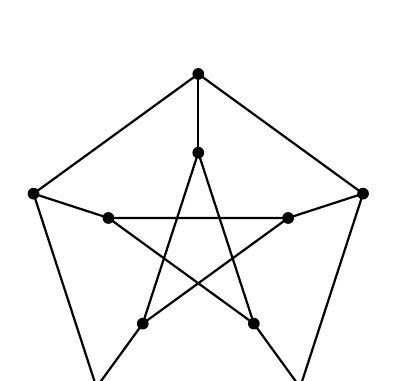
\begin{tikzpicture}[every path/.style=thick]
      \node[circle,fill,inner sep=1.5pt] at (90:2.2) {};
      \node[circle,fill,inner sep=1.5pt] at (162:2.2) {};
      \node[circle,fill,inner sep=1.5pt] at (234:2.2) {};
      \node[circle,fill,inner sep=1.5pt] at (306:2.2) {};
      \node[circle,fill,inner sep=1.5pt] at (18:2.2) {};

      \node[circle,fill,inner sep=1.5pt] at (90:1.2) {};
      \node[circle,fill,inner sep=1.5pt] at (162:1.2) {};
      \node[circle,fill,inner sep=1.5pt] at (234:1.2) {};
      \node[circle,fill,inner sep=1.5pt] at (306:1.2) {};
      \node[circle,fill,inner sep=1.5pt] at (18:1.2) {};

      \draw (90:2.2) -- (162:2.2) -- (234:2.2) -- (306:2.2) -- (18:2.2) -- (90:2.2);

      \draw (90:1.2) -- (306:1.2) -- (162:1.2) -- (18:1.2) -- (234:1.2) -- (90:1.2);

      \draw (90:2.2) -- (90:1.2);
      \draw (162:2.2) -- (162:1.2);
      \draw (234:2.2) -- (234:1.2);
      \draw (306:2.2) -- (306:1.2);
      \draw (18:2.2) -- (18:1.2);
  \end{tikzpicture}
  \end{center}
  This is known as the \textit{Petersen graph}.
  However, we must be careful.
  Recall that the Petersen graph is not a planar graph.
  This means that in the real plane, the $1$-cells must intersect,
  which means this is not a CW complex,
  but we can embed this graph (as well as any other finite graph) in $\R^3$
  without $1$-cells intersections,
  so it does have a CW complex representation. 
\end{example}

\begin{example}
  We can define a cellular complex for $S^2$
  by setting $X^{(0)} = \set{v}$
  and letting $X^{(1)}$ be $X^{(0)} \sqcup \D^1 / \varphi_1$
  where $\varphi_1 \colon \partial \D^1 \to \set{v}$
  is the constant map,
  and then gluing two more $2$-discs by attaching maps that
  send their boundaries to $\phi_1(\D^1)$.
  We get something like
  \[
    \tikz[eqpic]{
      \node[circle, fill, inner sep=1.5pt] (v) at (0,0) {};
    } \quad\taking{\qquad}\quad
    \tikz[eqpic,scale=0.7]{
      \node[circle, fill, inner sep=1.5pt] (v) at (2,0) {};
      \draw (-2,0) arc
        [start angle=180, end angle=360, x radius=2cm, y radius=0.35cm];
      \draw (2,0) arc
        [start angle=0, end angle=180, x radius=2cm, y radius=0.35cm];
    } \quad\taking{\qquad}\quad
    \tikz[eqpic,scale=0.7]{
      \node[circle, fill, inner sep=1.5pt] (v) at (2,0) {};
      \draw (-2,0) arc
        [start angle=180, end angle=360, x radius=2cm, y radius=0.35cm];
      \draw[dashed] (2,0) arc
        [start angle=0, end angle=180, x radius=2cm, y radius=0.35cm];
      \draw (0,0) circle (2cm);
    }
  \]
  Note that this is not a $\Delta$-complex.
\end{example}

\begin{example}
  \label{exmp:cw-for-sn-one-n-cell}
  We can also construct a cellular complex for $S^n$
  by setting $X^{(0)} = \set{x_0}$
  and $X^{(i)} = X^{(0)}$ for $1 \le i < k$,
  and then add a single $n$-cell by $(\D^n,\varphi)$
  so that $\varphi \colon \partial \D^n \to X$
  is the constant map $\varphi(x) = x_0$. 
  Note that this is not a $\Delta$-complex.
  The general construction looks like this:
  \[
    \tikz[eqpic]{
      \node[circle, fill, inner sep=1.5pt] (v) at (0,0) {};
    } \quad\taking{\qquad}\quad 
    \tikz[eqpic]{
      \node[circle, fill, inner sep=1.5pt] (v) at (0,0) {};
    } \quad\taking{\qquad}\quad \cdots \quad\taking{\qquad}\quad
    \tikz[eqpic]{
      \node[circle, fill, inner sep=1.5pt] (v) at (0,0) {};
    } \quad\taking{\qquad}\quad
    \text{$n$-sphere with a point}  
  \]
\end{example}

\begin{remark}
  We can also construct a CW complex for $S^2$ with many many cells,
  so that it looks like a basketball, or a soccer ball.
  We can also simply triangulize $S^2$ as we did for a $\Delta$-complex,
  however these methods will not prove very efficient when we will
  try to compute the homology of these complexes.
\end{remark}

\begin{example}
  \label{exmp:cw-for-torus}
  We can construct a CW complex for the torus $T^2$ by noticing that
  \[
    T^2 \,\,\cong\,\,
    \tikz[eqpic,scale=0.7]{
      \draw[pattern=north west lines,opacity=0.7,pattern color=green]
        (-2,-2) -- (-2,2) -- (2,2) -- (2,-2) -- cycle;
      \draw[->-=4/0.7,red] (-2,2) -- (2,2);
      \draw[-<-=4/0.7,blue] (2,2) -- (2,-2);
      \draw[-<-=4/0.7,red] (2,-2) -- (-2,-2);
      \draw[->-=4/0.7,blue] (-2,-2) -- (-2,2);
      \node[fill, circle, inner sep=1.5pt] (r1) at (-2,-2) {};
      \node[fill, circle, inner sep=1.5pt] (r2) at (2,2) {};
      \node[fill, circle, inner sep=1.5pt] (r3) at (2,-2) {};
      \node[fill, circle, inner sep=1.5pt] (r4) at (-2,2) {};
      \node[label=left:$a$] (a1) at (-2,0) {};
      \node[label=right:$a$] (a2) at (2,0) {};
      \node[label=above:$b$] (b1) at (0,2) {};
      \node[label=below:$b$] (b2) at (0,-2) {};
    }
    \,\, \cong\,\,
    \tikz[eqpic,scale=1.2]{
      \draw[pattern=north west lines,opacity=0.7,pattern color=green]
        (1,0) circle (1cm) {};
      \draw[pattern=north west lines,opacity=0.7,pattern color=green]
        (-1,0) circle (1cm) {};
      \begin{scope}[xscale=-1]
      \draw[blue,<--] (0:2) arc[start angle=0, end angle=-360, radius=1];
      \end{scope}
      \draw[red,-->] (0:2) arc[start angle=0, end angle=360, radius=1];
      \node[fill, circle, inner sep=1.5pt] (r1) at (0,0) {};
      \node[label=left:$a$] (a) at (-2,0) {};
      \node[label=right:$b$] (b) at (2,0) {};
    }
  \]
  so we just need a single $0$-cell denoted $e^0$,
  two $1$-cells denoted $e^1_a$ and $e^1_b$, with boundaries
  attached to $e^0$, and one $2$-cell denoted $e^2$,
  the attaching map gluing its boundary along the word
  $aba^{-1}b^{-1}$, where the loops $a$ and $b$ represent the $1$-cells
  $e^1_a$ and $e^1_b$ respectively.
\end{example}

\begin{example}
  The space $\RP^n$ is just the space of lines in $\R^{n+1}$
  passing through the origin $\R^{n+1} - \set{0} / x \sim \lambda x$.
  In particular, we get that $\RP^{0}$ is simply a point $\D^0 = \set{*}$.
  We also know that $\RP^{n}$ is homeomorohic to $S^n / x \sim -x$
  so for $\RP^{1}$ we get that
  \[
    \RP^1 =
    \tikz[eqpic]{
      \draw[<--] (90:1) arc[start angle=90, end angle=-90, radius=1];
      \draw[<--] (-90:1) arc[start angle=-90, end angle=-270, radius=1];
      \node[fill, circle, inner sep=1.5pt, label=left:$v$] (v1) at (-1,0) {};
      \node[fill, circle, inner sep=1.5pt, label=right:$v$] (v2) at (1,0) {};
    } =
    \tikz[eqpic]{
      \draw[-->] (90:0) arc[start angle=90, end angle=270+360, radius=1];
      \draw[-->] (0:0) arc[start angle=-90, end angle=90+360, radius=1];
      \node[fill, circle, inner sep=1.5pt, label=above:$v$] (v) at (0,0) {};
    } =
    \tikz[eqpic]{
      \draw[-->] (0:0) arc[start angle=90, end angle=90+360, radius=1];
      \node[fill, circle, inner sep=1.5pt, label=above:$v$] (v) at (0,-2) {};
    } = S^1
  \]
  so we have that $S^1 \cong \RP^1$ (but this is an anomaly).
  This shows that we can construct a CW complex for $\RP^1$
  by attaching one $1$-cell to one $0$-cell
  in the obvious way.
  Equivalently, by attaching one $1$-cell to $\RP^0$.
  When considering $\RP^2$,
  we get a $2$-sphere with identified antipodal points.
  This is equal to the upper hemisphere of the $2$-sphere,
  with the equator having its antipodal points glued together just like
  a copy of $\RP^1$.
  We will abuse notation and denote the equator of $\RP^2$ by $\RP^1$.
  \[
    \RP^2 =
    \tikz[eqpic,scale=0.7]{
      \draw (-2,0) arc
        [start angle=180, end angle=360, x radius=2cm, y radius=0.35cm];
      \draw[dashed] (2,0) arc
        [start angle=0, end angle=180, x radius=2cm, y radius=0.35cm];
      \draw (0,0) circle (2cm);
    } \,/\, \forall x(x \sim -x) =
    \tikz[eqpic,scale=0.7]{
      \draw (-2,0) arc
        [start angle=180, end angle=360, x radius=2cm, y radius=0.35cm];
      \draw[dashed] (2,0) arc
        [start angle=0, end angle=180, x radius=2cm, y radius=0.35cm];
      \draw[] (2,0) arc
        [start angle=0, end angle=180, radius=2cm];
    } \,/\,\forall x \in \RP^1(x \sim -x)
  \]
  This shows that we can construct a CW complex for $\RP^2$
  by attaching one $2$-cell to $\RP^1$.
  This pattern continues,
  and in this way we can construct a CW complex for $\RP^n$
  with one $i$-cell for all $0 \le i \le n$ for all $n$.
\end{example}

\begin{remark}
  Formally,
  the pattern for the inductive construction of real projective spaces is
  $\RP^n \cong \RP^{n-1} \sqcup \bigsqcup \D^n / \set{x \sim \varphi(x)}$
  with $\varphi_{\alpha} \colon \partial \D^n_{\alpha} \to \RP^{n-1}$
  defined in the natural way.
\end{remark}

\begin{exercise}
  \label{ex:cw-for-cp}
  Think of a CW complex for $\CP^n$
  (with a single cell in each even dimension).
  In particular, this implies that $\CP^1 \cong S^2$.
\end{exercise}

\subsection{Cellular homology}

\begin{remark}
  For all subcomplexes $A \subseteq X$ the pair $(X,A)$
  is a good pair.
\end{remark}

\begin{lemma}
  Let $X$ be a CW complex so that $X = \bigcup X^{(n)}$.
  \begin{enumerate}
    \item[(1)] We have that
      \[
        H_k\del[1]{X^{(n)},X^{(n-1)}} =
        \begin{cases}
          \bigoplus_{\alpha} \Z[\phi_{\alpha}], &n = k, \\
          0, & n \neq k.
        \end{cases}
      \]
      Note that $\phi_{\alpha}$ are the characteristic maps.
    \item[(2)] We have that $H_k(X^{(n)}) \cong \set{0}$ for $k > n$.
    \item[(3)] We have that $H_k(X^{(n)}) \cong H_k(X)$ for $n > k$.
  \end{enumerate}
\end{lemma}
\begin{proof} \phantom{}
\begin{enumerate}
  \item[(1)] Follows from the fact that $(X^{(n)},X^{(n-1)})$ is a good
    pair and that $X^{(n)} / X^{(n-1)}$ is a wedge of $n$-spheres.
    % Consider
    % $(\bigsqcup \D^n_{\alpha}, \bigsqcup \partial \D^n_{\alpha})$
    % sent by $(\phi_{\alpha},\varphi_{\alpha})$ to $(X^{(n)},X^{(n-1)})$.
    % We know that
    % \[
    %   \bigoplus
    %   H_k\del{\bigsqcup \D^n_{\alpha}, \bigsqcup \partial \D^n_{\alpha}}
    %   \cong
    %   H_k(\D^n_{\alpha}, \partial \D^n_{\alpha}).
    % \]
    % We get that
    % \[
    %   \widetilde H_k\del{\bigsqcup \D^n_{\alpha} /
    %     \bigsqcup \partial \D^n_{\alpha}}
    %   \cong
    %   \widetilde H_k(X^{(n)} / X^{(n-1)}).
    % \]
    % The projections $\bigoplus \Z[\phi_{\alpha}] \to \Z[\phi_{\alpha}]$
    % is induced by the map
    % $X^{(n)} \to X^{(n)} / X^{(n-1)} \to
    % \bigvee_{\beta} S^n_{\beta} / \bigvee_{\beta \neq \alpha} S^n_{\beta} \cong
    % S^n_{\alpha} \cong \D^n_{\alpha} / \partial \D^n_{\alpha}$.
    % where $\bigvee_{\beta} S^n_{\beta} / \bigvee_{\beta \neq \alpha} S^n_{\beta}$
    % is just a wedge of $S^n_{\beta}$.
  \item[(2)] Consider this subsequence of the
    long exact sequence of the pair $(X^{(n)}, X^{(n-1)})$:
    \[\begin{tikzcd}[ampersand replacement=\&,cramped]
      {(H_{k+1}X^{(n)},X^{(n-1)})} \& {H_{k}(X^{(n-1)})} \& {H_{k}(X^{(n)})} \& {H_{k}(X^{(n)},X^{(n-1)})}
      \arrow[from=1-1, to=1-2]
      \arrow[from=1-2, to=1-3]
      \arrow[from=1-3, to=1-4]
    \end{tikzcd}\]
    Since $k > n$ we get that $k \neq n$ and $k \neq n-1$ so
    \[
      H_{k+1}(X^{(n)},X^{(n-1)}) \cong
      H_{k}(X^{(n)},X^{(n-1)}) \cong \set{0}.
    \]
    By exactness of the sequence we get $H_k(X^{n-1}) \cong H_k(X^{(k)})$.
    Thus for $k > n$ we get
    \[
      H_k(X^{(n)}) \cong
      H_k(X^{(n-1)}) \cong \cdots \cong
      H_k(X^{(0)}) = \set{0},
    \]
    which completes the second part of the lemma.
  \item[(3)] For finite dimensional $X$ ($X = X^{(n)}$ for some $n$),
    the statement follows from the same long exact sequence from $(2)$.
  %   $H_k(X^{(n)}) \cong H_k(X^{(n-1)}) \cong \cdots \cong H_k(X^{(m)})$.
\end{enumerate}
\end{proof}

\begin{definition}[Cellular chains]
  We define
  $C_n^{\CW} = H_n(X^{(n)},X^{(n-1)})$
  Note that this implies that
  $C_n^{\CW} \cong \bigoplus_{\alpha} \Z[\phi_{\alpha}]$
  for characteristic maps $\phi_{\alpha}$ of $n$-cells.
  The chain groups $C^{\CW}_n(W)$ will form our cellular chain complex.
  \[\begin{tikzcd}[ampersand replacement=\&,cramped]
    \cdots \& {H_{n+1}(X^{n+1},X^{n})} \& {H_{n}(X^{n},X^{n-1})} \& {H_{n-1}(X^{n-1},X^{n-2})} \& \cdots
    \arrow[from=1-1, to=1-2]
    \arrow["{d_{n+1}}", from=1-2, to=1-3]
    \arrow["{d_n}", from=1-3, to=1-4]
    \arrow[from=1-4, to=1-5]
  \end{tikzcd}\]
\end{definition}

\begin{definition}[Cellular boundary map]
  We want to construct the boundary maps $d_n$.
  We notice that we can combine the long exact sequences of the pairs
  $(X^{n},X^{n-1})$ and $(X^{n-1},X^{n-2})$ to get a diagram
  of the form
  % https://q.uiver.app/#q=WzAsMTAsWzEsMiwiSF97bisxfShYXntuKzF9LFhee259KSJdLFsyLDIsIkhfe259KFhee259LFhee24tMX0pIl0sWzMsMiwiSF97bi0xfShYXntuLTF9LFhee24tMn0pIl0sWzAsMiwiXFxjZG90cyJdLFs0LDIsIlxcY2RvdHMiXSxbMSwxLCJIX24oWF5uKSJdLFsyLDMsIkhfe24tMX0oWF57bi0xfSkiXSxbMCwwLCIwIl0sWzIsMCwiSF9uKFhee24rMX0pIl0sWzEsNCwiMCJdLFszLDBdLFswLDEsImRfe24rMX0iXSxbMSwyLCJkX24iXSxbMiw0XSxbMCw1LCJcXHBhcnRpYWxfe24rMX0iXSxbNSwxLCJxX24iXSxbMSw2LCJcXHBhcnRpYWxfbiJdLFs2LDIsInFfe24tMX0iLDJdLFs3LDVdLFs1LDhdLFs5LDZdXQ==
  \[\begin{tikzcd}[ampersand replacement=\&,cramped]
    0 \&\& {H_n(X^{n+1})} \\
    \& {H_n(X^n)} \\
    \cdots \& {H_{n+1}(X^{n+1},X^{n})} \& {H_{n}(X^{n},X^{n-1})} \& {H_{n-1}(X^{n-1},X^{n-2})} \& \cdots \\
    \&\& {H_{n-1}(X^{n-1})} \\
    \& 0
    \arrow[from=1-1, to=2-2]
    \arrow[from=2-2, to=1-3]
    \arrow["{q_n}", from=2-2, to=3-3]
    \arrow[from=3-1, to=3-2]
    \arrow["{\partial_{n+1}}", from=3-2, to=2-2]
    \arrow["{d_{n+1}}", from=3-2, to=3-3]
    \arrow["{d_n}", from=3-3, to=3-4]
    \arrow["{\partial_n}", from=3-3, to=4-3]
    \arrow[from=3-4, to=3-5]
    \arrow["{q_{n-1}}"', from=4-3, to=3-4]
    \arrow[from=5-2, to=4-3]
  \end{tikzcd}\]
  We define $\partial^{\CW} := d_n = q_{n-1} \circ \partial_n$.
  Indeed we get
  $\del{\partial^{\CW}}^2 = q_* \circ \partial \circ q_* \circ \partial = 0$
  because of exactness and $\partial \circ q_* = 0$.
\end{definition}

\begin{remark}
  We want a practical way to compute the boundary maps $\partial^{\CW}_{n}$.
  Let $\varphi_{\alpha} \colon \partial \D^n_{\alpha} \to X^{(n-1)}$ be the
  attaching map of some $n$-cell.
  We then have the following sequence
  \[
    S^{n-1}_{\alpha} \cong
    \partial \D^n_{\alpha} \taking{\,\, \varphi_{\alpha} \,\,}
    X^{(n-1)} \taking{\,\, q \,\,}
    X^{(n-1)} / X^{(n-2)} \cong
    \bigvee_{\delta} S^{n-1}_{\delta} \taking{\,\, p_{\beta} \,\,}
    \bigvee_{\delta} S^{n-1}_{\delta} / \bigvee_{\delta \neq \beta}
      S^{n-1}_{\beta} \cong S^{n-1}_{\beta}.
  \]
  for each $(n-1)$-cell $\beta$.
  Define the map $\varphi_{\alpha \beta} \colon S^n_{\alpha} \to S^n_{\beta}$
  to be the composition of these maps.
  Then we have
  \[
    \partial^{\CW}\del{[\phi_{\alpha}]} =
    \sum_{\beta} \deg(\varphi_{\alpha \beta}) \cdot [\phi_{\beta}].
  \]
\end{remark}

\begin{remark}
  Earlier we have used both $d_n$ and $\partial^{\CW}_{n}$ interchangeably
  to denote the boundary map of the cellular chain complex.
  From now on we will only use $d_n$ for brevity.
\end{remark}

\begin{remark}
  In order to compute the cellular homology of spaces,
  the only facts we have to remember are that
  $C^{\CW}_n(X) = \bigoplus_{\alpha} \Z[\phi_{\alpha}]$
  where $\phi_{\alpha}$ are characteristic maps of $n$-cells,
  and that the boundary maps are given by
  \[
    d_n\del{[\phi_{\alpha}]} =
    \sum_{\beta} \deg(\varphi_{\alpha \beta}) \cdot [\phi_{\beta}].
  \]
\end{remark}

\begin{example}
  Let $X = S^n$ for $n \geq 2$.
  As we saw in \Cref{exmp:cw-for-sn-one-n-cell}
  we can construct a CW complex for $X$ using only
  one $0$-cell and one $n$-cell.
  The cellular chain of such a complex is of the form
  \[\begin{tikzcd}[ampersand replacement=\&,cramped]
    \cdots \& 0 \& \Z \& 0 \& \cdots \& 0 \& \Z \& 0
    \arrow[from=1-1, to=1-2]
    \arrow["d_{n+1}",from=1-2, to=1-3]
    \arrow["d_n",from=1-3, to=1-4]
    \arrow["d_{n-1}",from=1-4, to=1-5]
    \arrow["d_2",from=1-5, to=1-6]
    \arrow["d_1",from=1-6, to=1-7]
    \arrow["d_0",from=1-7, to=1-8]
  \end{tikzcd}\]
  We don't even have to compute the boundary maps since
  they are all simply the zero maps,
  and we immediately get that
  \[
    H_k^{\CW}(S^n) \cong
    \begin{cases}
      \Z, &k = 0 \stor k = n, \\
      0, &\text{otherwise}.
    \end{cases}
  \]
\end{example}

\begin{example}
  Let $X = \CP^n = \C^{n+1} - \set{0} / x \sim \lambda x$
  for $0 \neq \lambda \in \C$.
  Then from \Cref{ex:cw-for-cp}
  we know that $X$ has a CW complex with one $i$-cell for each $i = 2k$
  for $0 \le k \le n$.
  The cellular chain complex is
  \[\begin{tikzcd}[ampersand replacement=\&,cramped]
    \cdots \& 0 \& \Z \& 0 \& \cdots \& \Z \& 0 \& \Z \& 0
    \arrow[from=1-1, to=1-2]
    \arrow["d_{2n+1}",from=1-2, to=1-3]
    \arrow["d_{2n}",from=1-3, to=1-4]
    \arrow["d_{2n-1}",from=1-4, to=1-5]
    \arrow["d_{3}",from=1-5, to=1-6]
    \arrow["d_{2}",from=1-6, to=1-7]
    \arrow["d_{1}",from=1-7, to=1-8]
    \arrow["d_{0}",from=1-8, to=1-9]
  \end{tikzcd}\]
  and the homology is
  \[
    H_t^{\CW}(\CP^n) =
      \begin{cases}
        \Z, & t \le 2n \stand t \text{ even}, \\
        \set{0}, & \text{otherwise}.
      \end{cases}
  \]
\end{example}

\begin{example}
  \label{exmp:cw-for-torus-homology}
  Consider CW complex for the $2$-torus we saw in \Cref{exmp:cw-for-torus}
  \begin{center}
    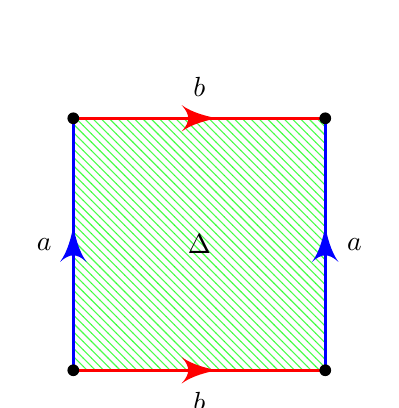
\begin{tikzpicture}[scale=0.8]
      \draw[pattern=north west lines,opacity=0.7,pattern color=green]
        (-2,-2) -- (-2,2) -- (2,2) -- (2,-2) -- cycle;
      \draw[->-=4/0.8,red] (-2,2) -- (2,2);
      \draw[-<-=4/0.8,blue] (2,2) -- (2,-2);
      \draw[-<-=4/0.8,red] (2,-2) -- (-2,-2);
      \draw[->-=4/0.8,blue] (-2,-2) -- (-2,2);
      \node[fill, circle, inner sep=1.5pt] (r1) at (-2,-2) {};
      \node[fill, circle, inner sep=1.5pt] (r2) at (2,2) {};
      \node[fill, circle, inner sep=1.5pt] (r3) at (2,-2) {};
      \node[fill, circle, inner sep=1.5pt] (r4) at (-2,2) {};
      \node[label=left:$a$] (a1) at (-2,0) {};
      \node[label=right:$a$] (a2) at (2,0) {};
      \node[label=above:$b$] (b1) at (0,2) {};
      \node[label=below:$b$] (b2) at (0,-2) {};
      \node[label=center:$\Delta$] (delta) at (0,0) {};
    \end{tikzpicture}
  \end{center}
  We can see that the cellular chain complex is of the form
  \[\begin{tikzcd}[ampersand replacement=\&,cramped]
    \cdots \& 0 \& {\Z\Delta} \& {\Z a \oplus \Z b} \& {\Z v} \& 0
    \arrow["d_{4}",from=1-1, to=1-2]
    \arrow["d_{3}",from=1-2, to=1-3]
    \arrow["d_{2}",from=1-3, to=1-4]
    \arrow["d_{1}",from=1-4, to=1-5]
    \arrow["d_{0}",from=1-5, to=1-6]
  \end{tikzcd}\]
  We know that CW complexes are the same as $\Delta$-complexes
  in dimensions $0$ and $1$ so in particular $d_1(a) = v - v = 0$
  and $d_1(b) = v - v = 0$.
  This means the only map which is (possibly) not the zero map in this chain
  is $d_2$.
  Using the formula for the boundary map we get
  \[
    d_2(\Delta) =
    \deg(\varphi_{\Delta a}) a +
    \deg(\varphi_{\Delta b}) b.
  \]
  In order to compute these degrees we can notice that
  \[
    \varphi_{\Delta a} \colon
    \partial \D_{\Delta}^2 \taking{\quad \varphi_{\Delta} \quad}
    X^{(1)} \cong
    \tikz[eqpic,scale=1]{
      \begin{scope}[xscale=-1]
      \draw[blue,<--] (0:2) arc[start angle=0, end angle=-360, radius=1];
      \end{scope}
      \draw[red,-->] (0:2) arc[start angle=0, end angle=360, radius=1];
      \node[fill, circle, inner sep=1.5pt] (r1) at (0,0) {};
      \node[label=left:$a$] (a) at (-2,0) {};
      \node[label=right:$b$] (b) at (2,0) {};
    } \taking{\quad p_a \quad}
    \tikz[eqpic,scale=1]{
      \begin{scope}[xscale=-1]
      \draw[blue,<--] (0:2) arc[start angle=0, end angle=-360, radius=1];
      \end{scope}
      \node[fill, circle, inner sep=1.5pt] (r1) at (0,0) {};
      \node[label=left:$a$] (a) at (-2,0) {};
    } = S^1_{a}
  \]
  Recall that $\varphi_{\Delta a}$ is a map between spheres,
  in particular $\varphi_{\Delta a} \colon S^1 \to S^1$,
  and we can see that it sends the boundary of $\D^2_{\Delta}$
  to a map which is homotopy equivalent to the constant map.
  \[
    \varphi_{\Delta a}\del{\,
    \tikz[eqpic,scale=0.5]{
      \draw[->-=4/0.5,red] (-2,2) -- (2,2);
      \draw[-<-=4/0.5,blue] (2,2) -- (2,-2);
      \draw[-<-=4/0.5,red] (2,-2) -- (-2,-2);
      \draw[->-=4/0.5,blue] (-2,-2) -- (-2,2);
      \node[fill, circle, inner sep=1.5pt] (r1) at (-2,-2) {};
      \node[fill, circle, inner sep=1.5pt] (r2) at (2,2) {};
      \node[fill, circle, inner sep=1.5pt] (r3) at (2,-2) {};
      \node[fill, circle, inner sep=1.5pt] (r4) at (-2,2) {};
  }\,} =
  \tikz[eqpic,scale=1]{
      \begin{scope}[xscale=-1]
      \draw[blue,<--] (0:2) arc[start angle=0, end angle=-360, radius=1];
      \end{scope}
      \draw[blue,-->] (0:2) arc[start angle=0, end angle=360, radius=1];
      \node[fill, circle, inner sep=1.5pt] (r1) at (0,0) {};
      \node[label=left:$a$] (a) at (-2,0) {};
      \node[label=right:$-a$] (b) at (2,0) {};
    } \simeq \bullet
  \]
  which, I admit, is a weird way to write that going over the boundary
  of the torus (which represents $S^1$) once, is mapped to
  going over $S^1_a$ once in some direction, and then in the opposite
  direction, which, as we know is homotopy equivalent to the constant map.
  This means that $\varphi_{\Delta a} \equiv 0$ and similarly
  $\varphi_{\Delta b} \equiv 0$.
  Since all boundary maps are the zero maps, we get
  \[
    H_k(T^2) =
    \begin{cases}
      \Z, & k = 0 \stor k = 2, \\
      \Z^2, & k = 1, \\
      \set{0}, &\text{otherwise}.
    \end{cases}
  \]
\end{example}

\begin{example}
  \label{exmp:homology-of-genus-two}
  Let $\Sigma_2 = T \# T$ be the compact orientable surface of genus two.
  I suggest looking for an online drawing of it,
  but here is its diagram as a quotient space
  \begin{center}
    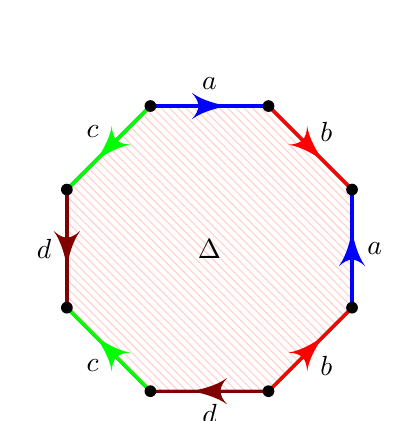
\begin{tikzpicture}

      \def\r{1.960}

      \draw[pattern=north west lines, pattern color=pink, opacity=0.7]
    ({\r*cos(22.5)},   {\r*sin(22.5)}) --
    ({\r*cos(67.5)},   {\r*sin(67.5)}) --
    ({\r*cos(112.5)},  {\r*sin(112.5)}) --
    ({\r*cos(157.5)},  {\r*sin(157.5)}) --
    ({\r*cos(202.5)},  {\r*sin(202.5)}) --
    ({\r*cos(247.5)},  {\r*sin(247.5)}) --
    ({\r*cos(292.5)},  {\r*sin(292.5)}) --
    ({\r*cos(337.5)},  {\r*sin(337.5)}) -- cycle;

      \draw[-<-={1.5},red]
        ({\r*cos(22.5)},  {\r*sin(22.5)})  -- ({\r*cos(67.5)},   {\r*sin(67.5)});
      \draw[-<-={1.5},blue]
        ({\r*cos(67.5)},  {\r*sin(67.5)})  -- ({\r*cos(112.5)},  {\r*sin(112.5)});
      \draw[->-={1.5},green]
        ({\r*cos(112.5)}, {\r*sin(112.5)}) -- ({\r*cos(157.5)},  {\r*sin(157.5)});
      \draw[->-={1.5},mred]
        ({\r*cos(157.5)}, {\r*sin(157.5)}) -- ({\r*cos(202.5)},  {\r*sin(202.5)});
      \draw[-<-={1.5},green]
        ({\r*cos(202.5)}, {\r*sin(202.5)}) -- ({\r*cos(247.5)},  {\r*sin(247.5)});
      \draw[-<-={1.5},mred]
        ({\r*cos(247.5)}, {\r*sin(247.5)}) -- ({\r*cos(292.5)},  {\r*sin(292.5)});
      \draw[->-={1.5},red]
        ({\r*cos(292.5)}, {\r*sin(292.5)}) -- ({\r*cos(337.5)},  {\r*sin(337.5)});
      \draw[->-={1.5},blue] 
        ({\r*cos(337.5)}, {\r*sin(337.5)}) -- ({\r*cos(22.5)},   {\r*sin(22.5)});

      \node[fill, circle, inner sep=1.5pt] at ({\r*cos(22.5)},   {\r*sin(22.5)})   {};
      \node[fill, circle, inner sep=1.5pt] at ({\r*cos(67.5)},   {\r*sin(67.5)})   {};
      \node[fill, circle, inner sep=1.5pt] at ({\r*cos(112.5)},  {\r*sin(112.5)})  {};
      \node[fill, circle, inner sep=1.5pt] at ({\r*cos(157.5)},  {\r*sin(157.5)})  {};
      \node[fill, circle, inner sep=1.5pt] at ({\r*cos(202.5)},  {\r*sin(202.5)})  {};
      \node[fill, circle, inner sep=1.5pt] at ({\r*cos(247.5)},  {\r*sin(247.5)})  {};
      \node[fill, circle, inner sep=1.5pt] at ({\r*cos(292.5)},  {\r*sin(292.5)})  {};
      \node[fill, circle, inner sep=1.5pt] at ({\r*cos(337.5)},  {\r*sin(337.5)})  {};

      \def\R{2.1}
      \node[inner sep=1.5pt, label=center:$a$] at ({\R*cos(0)},     {\R*sin(0)})     {};
      \node[inner sep=1.5pt, label=center:$b$] at ({\R*cos(45)},    {\R*sin(45)})    {};
      \node[inner sep=1.5pt, label=center:$a$] at ({\R*cos(90)},    {\R*sin(90)})    {};
      \node[inner sep=1.5pt, label=center:$c$] at ({\R*cos(135)},   {\R*sin(135)})   {};
      \node[inner sep=1.5pt, label=center:$d$] at ({\R*cos(180)},   {\R*sin(180)})   {};
      \node[inner sep=1.5pt, label=center:$c$] at ({\R*cos(225)},   {\R*sin(225)})   {};
      \node[inner sep=1.5pt, label=center:$d$] at ({\R*cos(270)},   {\R*sin(270)})   {};
      \node[inner sep=1.5pt, label=center:$b$] at ({\R*cos(315)},   {\R*sin(315)})   {};

      \node[inner sep=1.5pt, label=center:$\Delta$] at (0,0) {};

    \end{tikzpicture}
  \end{center}
  with all the vertices identified and denoted by $v$.
  The cellular chain complex is
  \[\begin{tikzcd}[ampersand replacement=\&,cramped]
    \cdots \& 0 \& {\Z \Delta} \& {\Z a \oplus \Z b \oplus \Z c \oplus \Z d} \& {\Z v} \& 0
    \arrow[from=1-1, to=1-2]
    \arrow["d_{3}",from=1-2, to=1-3]
    \arrow["d_{2}",from=1-3, to=1-4]
    \arrow["d_{1}",from=1-4, to=1-5]
    \arrow["d_{0}",from=1-5, to=1-6]
  \end{tikzcd}\]
  It is clear that all maps except (possibly) $d_2$ are zero maps.
  Similarly to what we saw in \Cref{exmp:cw-for-torus-homology}
  we get that
  \[
    \varphi_{\Delta a}\del{\,
    \tikz[eqpic,scale=0.7]{
      \def\r{1.960}
      \draw[-<-={1.5/0.7},red]
        ({\r*cos(22.5)},  {\r*sin(22.5)})  -- ({\r*cos(67.5)},   {\r*sin(67.5)});
      \draw[-<-={1.5/0.7},blue]
        ({\r*cos(67.5)},  {\r*sin(67.5)})  -- ({\r*cos(112.5)},  {\r*sin(112.5)});
      \draw[->-={1.5/0.7},green]
        ({\r*cos(112.5)}, {\r*sin(112.5)}) -- ({\r*cos(157.5)},  {\r*sin(157.5)});
      \draw[->-={1.5/0.7},mred]
        ({\r*cos(157.5)}, {\r*sin(157.5)}) -- ({\r*cos(202.5)},  {\r*sin(202.5)});
      \draw[-<-={1.5/0.7},green]
        ({\r*cos(202.5)}, {\r*sin(202.5)}) -- ({\r*cos(247.5)},  {\r*sin(247.5)});
      \draw[-<-={1.5/0.7},mred]
        ({\r*cos(247.5)}, {\r*sin(247.5)}) -- ({\r*cos(292.5)},  {\r*sin(292.5)});
      \draw[->-={1.5/0.7},red]
        ({\r*cos(292.5)}, {\r*sin(292.5)}) -- ({\r*cos(337.5)},  {\r*sin(337.5)});
      \draw[->-={1.5/0.7},blue] 
        ({\r*cos(337.5)}, {\r*sin(337.5)}) -- ({\r*cos(22.5)},   {\r*sin(22.5)});

      \node[fill, circle, inner sep=1.5pt] at ({\r*cos(22.5)},   {\r*sin(22.5)})   {};
      \node[fill, circle, inner sep=1.5pt] at ({\r*cos(67.5)},   {\r*sin(67.5)})   {};
      \node[fill, circle, inner sep=1.5pt] at ({\r*cos(112.5)},  {\r*sin(112.5)})  {};
      \node[fill, circle, inner sep=1.5pt] at ({\r*cos(157.5)},  {\r*sin(157.5)})  {};
      \node[fill, circle, inner sep=1.5pt] at ({\r*cos(202.5)},  {\r*sin(202.5)})  {};
      \node[fill, circle, inner sep=1.5pt] at ({\r*cos(247.5)},  {\r*sin(247.5)})  {};
      \node[fill, circle, inner sep=1.5pt] at ({\r*cos(292.5)},  {\r*sin(292.5)})  {};
      \node[fill, circle, inner sep=1.5pt] at ({\r*cos(337.5)},  {\r*sin(337.5)})  {}; 
  }\,} =
  \tikz[eqpic,scale=1]{
      \begin{scope}[xscale=-1]
      \draw[blue,<--] (0:2) arc[start angle=0, end angle=-360, radius=1];
      \end{scope}
      \draw[blue,-->] (0:2) arc[start angle=0, end angle=360, radius=1];
      \node[fill, circle, inner sep=1.5pt] (r1) at (0,0) {};
      \node[label=left:$a$] (a) at (-2,0) {};
      \node[label=right:$-a$] (b) at (2,0) {};
    } \simeq \bullet
  \]
  and so similarly $\varphi_{\Delta a}$, $\varphi_{\Delta b}$,
  $\varphi_{\Delta c}$ and $\varphi_{\Delta d}$ are all zero maps
  so $d_2 \equiv 0$ which means that
  \[
    H_n(\Sigma_2) =
    \begin{cases}
      \Z, &n = 0 \stor n = 2, \\
      \Z^4, &n = 1 \\
      \set{0}, &\text{otherwise}.
    \end{cases}
  \]
\end{example}

\begin{remark}
  The argument we saw in \Cref{exmp:homology-of-genus-two}
  does not actually depend on the assumption that the genus of
  the surface is $2$.
  Thus, we can generalize and say that in the case of the compact orientable
  surface of genus $g$, which is $\Sigma_{g} = \#^{g} T^2$,
  we have
  \[
    H_n(\Sigma_g) =
    \begin{cases}
      \Z, &n = 0 \stor n = 2, \\
      \Z^{2g}, &n = 1 \\
      \set{0}, &\text{otherwise}.
    \end{cases}
  \]
\end{remark}

\begin{example}
  Consider the Klein bottle $K$ with the CW complex
  \begin{center}
    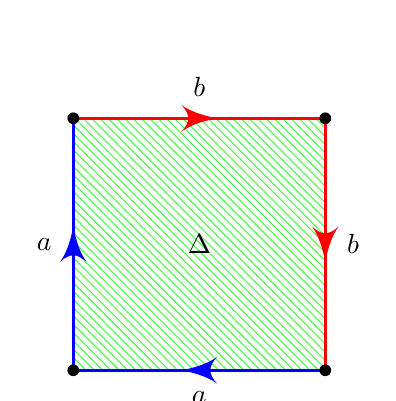
\begin{tikzpicture}[scale=0.8]
      \draw[pattern=north west lines,opacity=0.7,pattern color=green]
        (-2,-2) -- (-2,2) -- (2,2) -- (2,-2) -- cycle;
      \draw[->-=4/0.8,red] (-2,2) -- (2,2);
      \draw[->-=4/0.8,red] (2,2) -- (2,-2);
      \draw[->-=4/0.8,blue] (2,-2) -- (-2,-2);
      \draw[->-=4/0.8,blue] (-2,-2) -- (-2,2);
      \node[fill, circle, inner sep=1.5pt] (r1) at (-2,-2) {};
      \node[fill, circle, inner sep=1.5pt] (r2) at (2,2) {};
      \node[fill, circle, inner sep=1.5pt] (r3) at (2,-2) {};
      \node[fill, circle, inner sep=1.5pt] (r4) at (-2,2) {};
      \node[label=left:$a$] (a1) at (-2,0) {};
      \node[label=right:$b$] (a2) at (2,0) {};
      \node[label=above:$b$] (b1) at (0,2) {};
      \node[label=below:$a$] (b2) at (0,-2) {};
      \node[label=center:$\Delta$] (delta) at (0,0) {};
    \end{tikzpicture}
  \end{center}
  This is not the standard representation of the Klein bottle,
  but it is possible to get to the more standard representation
  but cutting along the anti diagonal and pasting along the side $a$.
  Using our representation we get a cellular chain complex of the form 
  \[\begin{tikzcd}[ampersand replacement=\&,cramped]
    \cdots \& 0 \& {\Z \Delta} \& {\Z a \oplus \Z b} \& {\Z v} \& 0
    \arrow["d_{4}",from=1-1, to=1-2]
    \arrow["d_{3}",from=1-2, to=1-3]
    \arrow["d_{2}",from=1-3, to=1-4]
    \arrow["d_{1}",from=1-4, to=1-5]
    \arrow["d_{0}",from=1-5, to=1-6]
  \end{tikzcd}\]
  As in all of the examples we have seen so far, the interesting map is $d_2$.
  This time, things are a little different.
  We have
  \[
    \varphi_{\Delta a} \colon
    \partial \D_{\Delta}^2 \taking{\quad \varphi_{\Delta} \quad}
    X^{(1)} \cong
    \tikz[eqpic,scale=1]{
      \begin{scope}[xscale=-1]
      \draw[blue,<--] (0:2) arc[start angle=0, end angle=-360, radius=1];
      \end{scope}
      \draw[red,<--] (0:2) arc[start angle=0, end angle=360, radius=1];
      \node[fill, circle, inner sep=1.5pt] (r1) at (0,0) {};
      \node[label=left:$a$] (a) at (-2,0) {};
      \node[label=right:$b$] (b) at (2,0) {};
    } \taking{\quad p_a \quad}
    \tikz[eqpic,scale=1]{
      \begin{scope}[xscale=-1]
      \draw[blue,<--] (0:2) arc[start angle=0, end angle=-360, radius=1];
      \end{scope}
      \node[fill, circle, inner sep=1.5pt] (r1) at (0,0) {};
      \node[label=left:$a$] (a) at (-2,0) {};
    } = S^1_{a}
  \]
  and
  \[
    \varphi_{\Delta a}\del{\,
    \tikz[eqpic,scale=0.5]{
      \draw[->-=4/0.5,red] (-2,2) -- (2,2);
      \draw[->-=4/0.5,red] (2,2) -- (2,-2);
      \draw[->-=4/0.5,blue] (2,-2) -- (-2,-2);
      \draw[->-=4/0.5,blue] (-2,-2) -- (-2,2);
      \node[fill, circle, inner sep=1.5pt] (r1) at (-2,-2) {};
      \node[fill, circle, inner sep=1.5pt] (r2) at (2,2) {};
      \node[fill, circle, inner sep=1.5pt] (r3) at (2,-2) {};
      \node[fill, circle, inner sep=1.5pt] (r4) at (-2,2) {};
  }\,} =
  \tikz[eqpic,scale=1]{
      \begin{scope}[xscale=-1]
      \draw[blue,<--] (0:2) arc[start angle=0, end angle=-360, radius=1];
      \end{scope}
      \draw[blue,<--] (0:2) arc[start angle=0, end angle=360, radius=1];
      \node[fill, circle, inner sep=1.5pt] (r1) at (0,0) {};
      \node[label=left:$a$] (a) at (-2,0) {};
      \node[label=right:$a$] (b) at (2,0) {};
    } \simeq z^2
  \]
  so $\varphi_{\Delta a}$ sends the boundary of the Klein bottle
  (one trip around $S^1 \cong \partial \D_{\Delta}^2$)
  to two trips around $S^1_{a}$ (just like $z^2$)
  and so $\deg(\varphi_{\Delta a}) = 2$.
  Similarly we get that $\deg(\varphi_{\Delta a}) = 2$,
  and thus we have
  \[
    d_2(\Delta) = 2 (a + b).
  \]
  Therefore the only nontrivial homology we have to calculate is
  \[
    H_1(K) =
    \frac{\ker d_{1}}{\im d_{2}} =
    \frac{\Z a \oplus \Z b}{\Z(2(a + b))} =
    \langle a,a+b \mid 2(a+b) \rangle =
    \langle a \rangle \oplus \langle a+b \mid 2(a+b) \rangle \cong
    Z \oplus \Z/2\Z.
  \]
  Therefore
  \[
    H_n(K) =
    \begin{cases}
      \Z, &n = 0, \\
      \Z \oplus \Z/2\Z, &n = 1, \\
      \set{0}, &\text{otherwise}.
    \end{cases}
  \]
\end{example}

\begin{example}
  \label{exmp:homology-of-rpn}
  Let $X = \RP^n$.
  We know that $X$ has a CW complex with one $i$-cell in each dimension
  $0 \le i \le n$.
  Thus the cellular chain complex is
  \[\begin{tikzcd}[ampersand replacement=\&,cramped]
    \cdots \& 0 \& \Z \& \cdots \& \Z \& \Z \& 0
    \arrow["d_{n+2}",from=1-1, to=1-2]
    \arrow["d_{n+1}",from=1-2, to=1-3]
    \arrow["d_{n}",from=1-3, to=1-4]
    \arrow["d_{2}",from=1-4, to=1-5]
    \arrow["d_{1}",from=1-5, to=1-6]
    \arrow["d_{0}",from=1-6, to=1-7]
  \end{tikzcd}\]
  It is not so clear what the boundary maps are anymore.
  Recall that
  \[
    S^{n-1}_{\alpha} \cong
    \partial \D^n_{\alpha} \taking{\,\, \varphi_{\alpha} \,\,}
    X^{(n-1)} \taking{\,\, q \,\,}
    X^{(n-1)} / X^{(n-2)} \cong
    \bigvee_{\delta} S^{n-1}_{\delta} \taking{\,\, p_{\beta} \,\,}
    \bigvee_{\delta} S^{n-1}_{\delta} / \bigvee_{\delta \neq \beta}
      S^{n-1}_{\beta} \cong S^{n-1}_{\beta}.
  \]
  so in our case since $X^{(n)} = \RP^{n}$ and there's only one
  cell in each dimension we get
  \[
    \varphi_{\Delta_n \Delta_{n-1}} \colon
    S^{n-1} \cong
    \partial \D^n \taking{\quad \varphi_{\Delta_n} \quad}
    \RP^{n-1} \taking{\quad q \quad}
    \RP^{n-1} / \RP^{n-2} \cong
    S^{n-1} 
  \]
  and 
  \[
    d_n\del{[\phi_{\Delta_n}]} =
    \sum_{\beta}
      \deg(\varphi_{\Delta_n \Delta_{n-1}}) \cdot [\phi_{\Delta_{n-1}}] =
    \deg(\varphi_{\Delta_n \Delta_{n-1}}) \cdot [\phi_{\Delta_{n-1}}],
  \]
  where $\Delta_n$ represents the $n$-cell of the complex.
  Note that the attaching map
  $\varphi_{\Delta_n} \colon S^{n-1} \to S^{n-1} / x \sim - x \cong \RP^{n-1}$
  is given by the canonical double cover of $\RP^{n-1}$.
  We now use \Cref{prop:local-degree-for-global-degree}.
  Let $y \in S^{n-1}$ not on the equator,
  then $\varphi^{-1}_{\Delta_n \Delta_{n-1}}(y) = \set{x,-x}$
  for some $x \in S^1$.
  This means that
  \[
    \deg(\varphi_{\Delta_n \Delta_{n-1}}) =
    \deg(\varphi_{\Delta_n \Delta_{n-1}}\vert_{x}) +
    \deg(\varphi_{\Delta_n \Delta_{n-1}}\vert_{-x}).
  \]
  However from the multiplicativity of the degree
  $\deg(\varphi_{\Delta_n \Delta_{n-1}}\vert_{-x}) =
  \deg(\varphi_{\Delta_n \Delta_{n-1}}\vert_{x}) \cdot \deg(\alpha \vert_{-x})$
  where $\alpha$ is the antipodal map.
  Since we know that $\varphi_{\Delta_n \Delta_{n-1}}$
  is homotopy equivalent to the identity in a sufficiently small
  neighbourhood of $x$,
  and that $\deg(\alpha \vert_{-x}) = (-1)^{n}$.
  It follows that $\deg(d_n) = 2$ when $n$ is even
  and $\deg(d_n) = 0$ when $n$ is odd.
  This implies that when $n$ is odd
  \[
    H_k(\RP^n) =
    \begin{cases}
      \Z, &k = 0 \stand k = n, \\
      \Z/2\Z, &0 < k < n \stand \text{$k$ is odd}, \\
      \set{0}, &\text{otherwise}.
    \end{cases}
  \]
  and when $n$ is even
  \[
    H_k(\RP^n) =
    \begin{cases}
      \Z, &k = 0, \\
      \Z/2\Z, &0 < k < n \stand \text{$k$ is odd}, \\
      \set{0}, &\text{otherwise}.
    \end{cases}
  \]
\end{example}

\subsection{Extras before cohomology}

\begin{definition}[Euler characteristic]
  Let $X$ be a CW complex with finitely many cells.
  Then we define the Euler characterstic of $X$ to be
  \[
    \chi(X) =
    \sum_{i=0}^{\infty} (-1)^i \#\set{\text{$i$-cells in $X$}} =
    \#\text{Vertices} - \#\text{Edges} + \#\text{2-faces} -
    \cdots
  \]
\end{definition}

\begin{theorem}
  The number $\chi(X)$ is independent of the CW complex on $X$.
  Moreover, if $X \simeq Y$ where $X$ and $Y$ are finite CW complexes,
  then $\chi(X) = \chi(Y)$.
\end{theorem}

\begin{definition}[Rank]
  Let $A$ be a finitely generated abelian group.
  Then from the classification of finitely generated abelian groups
  \[
    A = \Z^r \oplus B
  \]
  for some finite group $B$ and some $r \geq 0$.
  We define $\rank(A) = r$.
\end{definition}

\begin{exercise}
  \label{ex:fga-groups-ranks}
  Let
  \[\begin{tikzcd}[ampersand replacement=\&,cramped]
	0 \& A \& B \& C \& 0
	\arrow[from=1-1, to=1-2]
	\arrow[from=1-2, to=1-3]
	\arrow[from=1-3, to=1-4]
	\arrow[from=1-4, to=1-5]
\end{tikzcd}\]
  be a short exact sequence of abelian groups.
  Then $\rank(B) = \rank(A) + \rank(C)$.
\end{exercise}

\begin{theorem}
  Let $X$ be a finite CW complex.
  Then
  \[
    \chi(X) =
    \sum_{i=0}^{\infty} (-1)^i \rank\del{H_i(X)}
  \]
  where $H_i(X)$ are finitely generated because $C_i^{\CW}$ is finitely
  generated.
\end{theorem}
\begin{proof}
  We have the chain complex
  \[\begin{tikzcd}[ampersand replacement=\&,cramped]
    \cdots \& {C_{i+1}^{\CW}} \& {C_{i}^{\CW}} \& {C_{i-1}^{\CW}} \& \cdots
    \arrow[from=1-1, to=1-2]
    \arrow["{d_{i+1}}", from=1-2, to=1-3]
    \arrow["{d_i}", from=1-3, to=1-4]
    \arrow[from=1-4, to=1-5]
  \end{tikzcd}\]
  so in general if we denote $B_n = \im d_{n+1}$ 
  and $Z_n = \ker d_n$ so that $H_n = Z_n/B_n$
  we get the short exact sequences
  \[\begin{tikzcd}[ampersand replacement=\&,cramped]
    0 \& {B_i} \& {Z_i} \& {H^{\CW}_{i}(X)} \& 0
    \arrow[from=1-1, to=1-2]
    \arrow[from=1-2, to=1-3]
    \arrow[from=1-3, to=1-4]
    \arrow[from=1-4, to=1-5]
  \end{tikzcd}\]
  and
  \[\begin{tikzcd}[ampersand replacement=\&,cramped]
    0 \& {Z_{i}} \& {C^{\CW}_{i}(X)} \& {B_{i-1}} \& 0
    \arrow[from=1-1, to=1-2]
    \arrow[from=1-2, to=1-3]
    \arrow[from=1-3, to=1-4]
    \arrow[from=1-4, to=1-5]
  \end{tikzcd}\]
  so from \Cref{ex:fga-groups-ranks}
  we obtain the formulas
  \begin{gather*}
    \rank(Z_i) = \rank(B_i) + \rank(H_i) \\
    \rank(C_{i}^{\CW}) = \rank(B_{i-1}) + \rank(Z_{i})
  \end{gather*}
  so by simple arithmetic calculations
  \begin{align*}
    \chi(X) &=
    \sum_{i=0}^{\infty} (-1)^i \#\set{\text{$i$-cells in $X$}} \\ &=
    \sum_{i=0}^{\infty} (-1)^i \del{\rank(B_{i-1}) + \rank(Z_i)} \\ &=
    \sum_{i=0}^{\infty} (-1)^i
      \del{\rank(Z_{i-1}) - \rank(H_{i-1}) + \rank(Z_i)} \\ &=
    \sum_{i=0}^{\infty} (-1)^{i-1} \rank\del{H_{i-1}(X)}
  \end{align*}
  where the last step follows from the fact the series is a telescopic
  sum.
\end{proof}

\begin{remark}
  In every odd dimension the Euler characteristic of any compact
  manifold is zero.
\end{remark}

\begin{theorem}[Jordan curve theorem]
  Let $h \colon S^1 \to S^2$. Then $h(S^1)$ decomposes $S^2$
  into two path connected components.
  Formally, $S^2 - h(S^1)$ has two path connected components,
  or in the language of homology, $\widetilde H_0(S^2 - h(S^1)) = \Z$.
\end{theorem}
\begin{theorem}[Jordan--Schoenflies]
  Let $h \colon S^1 \to S^2$.
  Then $h$ can be extended to a homeomorphism $H \colon S^2 \taking{\cong} S^2$
  so that $H\vert_{E} = h$, where $E \cong S^1$ is the equator of $S^2$.
\end{theorem}

\begin{example}
  This theorem can not be generalized to higher dimensions.
  Let $h(S^2) \subset S^3$ be Alexander's horned sphere.
  It's a counterexample, it's very hard to draw here just look it up.
  % to be added
\end{example}

\begin{theorem} \phantom{}
  \begin{enumerate}
    \item[(1)] Let $h \colon \D^k \hookrightarrow S^n$ be a continuous map.
      Then $\widetilde H_i(S^n - h(\D^k)) = 0$ for all $i$.
    \item[(2)] Let $h \colon S^k \hookrightarrow S^n$
      be a continuous map so that $k < n$. Then
      \[
        \widetilde H_i(S^n - h(S^k)) \cong
        \begin{cases}
          \Z, &i = n - k - 1, \\
          0, &\text{otherwise}.
        \end{cases}
      \]
  \end{enumerate}
\end{theorem}
\begin{proof} \phantom{}
  \begin{enumerate}
    \item[(1)] We prove this by induction on $k$.
      When $k = 0$ we have $\D^k = \set{*}$
      and then $S^n - \set{*} \cong \R^n$ so since this is contractible
      $\widetilde H_i(S^n - h(\D^k)) = \widetilde H_i(\R^n) = 0$ for all $i$.

      Next we identify $\D^k \cong [0,1]^k = I^k$.
      Define
      \begin{gather*}
        A' = [0,1/2] \times I^{k-1} \\
        B' = [1/2,1] \times I^{k-1}
      \end{gather*}
      Then we define $A = S^n - h(A')$ and $B = S^n - h(B')$
      which are open.
      We then have $A \cap B = S^n - h(I^k)$ which
      means we want to compute $\widetilde H_{i}(A \cap B)$.
      In order to use Mayer--Vietoris we compute the union
      $A \cup B = S^n - h(A \cap B) = S^n - \set{1/2} \times I^{k-1}$.
      Then from Mayer--Vietoris we get
      % https://q.uiver.app/#q=WzAsNixbMSwwLCJcXHdpZGV0aWxkZSBIX3tpKzF9KEEgXFxjdXAgQikiXSxbMiwwLCJcXHdpZGV0aWxkZSBIX3tpfShBIFxcY2FwIEIpIl0sWzMsMCwiXFx3aWRldGlsZGUgSF97aX0oQSkgXFxvcGx1cyBcXHdpZGV0aWxkZSBIX3tpfShCKSJdLFs0LDAsIlxcd2lkZXRpbGRlIEhfe2l9KEEgXFxjdXAgQikiXSxbMCwwLCJcXGNkb3RzIl0sWzUsMCwiXFxjZG90cyJdLFs0LDBdLFswLDFdLFsxLDJdLFsyLDNdLFszLDVdXQ==
\[\begin{tikzcd}[ampersand replacement=\&,cramped]
	\cdots \& {\widetilde H_{i+1}(A \cup B)} \& {\widetilde H_{i}(A \cap B)} \& {\widetilde H_{i}(A) \oplus \widetilde H_{i}(B)} \& {\widetilde H_{i}(A \cup B)} \& \cdots
	\arrow[from=1-1, to=1-2]
	\arrow[from=1-2, to=1-3]
	\arrow[from=1-3, to=1-4]
	\arrow[from=1-4, to=1-5]
	\arrow[from=1-5, to=1-6]
\end{tikzcd}\]
  but since the groups at the edges are trivial we have
  $\widetilde H_{i}(A \cap B) \cong
  \widetilde H_{i}(A) \oplus \widetilde H_{i}(B)$.
  Assume, by way of contradiction, that $\widetilde H_{i}(A \cap B)$
  is not trivial.
  Then there exists $0 \neq c \in \widetilde H_{i}(A \cap B)$
  so that either $0 \neq c \in \widetilde H_{i}(A)$ or
  $0 \neq c \in \widetilde H_{i}(B)$.
  In the first case denote $A_1 = A$, in the second $A_1 = B$.
  Continue the process on $A_1$ instead of $S^n$
  and so on indefinitely to get a sequence
  $A_1 \subseteq \cdots \subseteq A_n \subseteq \cdots$
  so that $A'_1 \supseteq \cdots \supseteq A'_n \supseteq$ indefinitely.
  Then we have $\bigcap A'_n = \set{*} \times I^{k-1}$.
  This implies that
  $0 \neq c \in \widetilde H_i(S^n - h(\set{*} \times I^{k-1})) = 0$,
  but by the induction hypothesis we get that $c = \partial d$ for some
  $d \in C_{i+1}(S^n - h(\set{*} \times I^{k-1}))$.
  to be finished.
    \item[(2)] We know that $S^k = D_1 \sqcup D_2$ for some $k$-discs
      glued at their boundary.
      Then again by letting
      \begin{gather*}
        A = S^n - h(D_1) \\
        B = S^n - h(D_2)
      \end{gather*}
      we get from Mayer--Vietrois and part $(1)$ the desired
      isomorphism.
  \end{enumerate}
\end{proof}

\begin{definition}[Wild knot]
  An embedding $h \colon S^1 \hookrightarrow S^3$ is called a wild knot.
\end{definition}

\begin{remark}
  A wild knot is a called ``wild'' because it can be very pathological.
  A knot that is not wild is called tame.
  One way to rid the knot of pathological behaviour,
  is by requiring it to be smooth.
  Smooth knots are not the only tame knots.
\end{remark}

\begin{corollary}
  Let $h$ be a wild knot.
  Then $\widetilde H_i(S^3 - h(S^1)) = \Z$.
\end{corollary}

\begin{remark}
  In modern terminology a domain $U$ is an open connected set.
  A long time ago a domain was just another term for an open set.
\end{remark}

\begin{theorem}[Invariance of domain]
  \label{thm:invariance-of-domain}
  Let $U \subseteq \R^n$ be an open set and let
  $f \colon U \to \R^n$ be a continuous and injective map.
  Then $f(U) \subseteq \R^n$ is open.
  It follows that $f$ is an open map.
\end{theorem}
\begin{proof}
  We know that $\R^n \subset S^n$.
  We will show that $f \colon U \to S^n$ is open.
  Let $x \in \D \subset U$.
  We have $\D = \D^n \subseteq \R^n$.
  From the previous Jordan theorem we know that
  the $n - (n - 1) - 1 = 0$th homology is
  \[
    \widetilde H_0(S^n - f(\partial \D)) = \Z.
  \]
  This means that $S^n - f(\partial \D)$ has two path connected components.
  We know that the path connected components are
  \[
    \begin{cases}
      f(\D - \partial \D) \\
      S^n - f(\D)
    \end{cases}
  \]
  Since path connected components of a locally path connected space are open,
  thus in particular $f(\D - \partial \D) =  f(\mathring \D)$ is open.
  % to be processed
\end{proof}

\begin{definition}[Topological $n$-manifold]
  Let $M$ be a second countable Hausdorff space.
  Then $M$ is said to be an $n$-manifold if $M$
  is locally homeormophic to $\R^n$.
  Moreover, $M$ is a closed $n$-manifold if $M$ is compact.
\end{definition}

\begin{theorem}
  Let $N$ and $M$ be closed connected $n$-manifolds
  and let $f \colon M \to N$ be a continuous injective map.
  Then $f$ is a homeomorphism.
\end{theorem}
\begin{proof}
  From \Cref{thm:invariance-of-domain} $f$ is open.
  Thus $f(M)$ is open and closed.
  Since $N$ is connected, it follows that $f(M) = N$.
\end{proof}

\subsection{Homology with coefficients}
\begin{remark}
  $\Z$ is the most important group in the world.
\end{remark}
\begin{remark}
  Let $(G,+)$ be an abelian group.
  Then we can define $C_n(X;G) = \bigoplus G\sigma$.
  This chain complex induces homology groups $H_n(X;G)$.
\end{remark}
\begin{remark}
  All previous propositions and theorems like excision,
  Mayer--Vietoris still apply when doing homology with coefficients.
\end{remark}
\begin{remark}
  Let $f \colon S^n \to S^n$ be a map.
  We then have $f_* \colon H_n(S^n ; G) \to H_n(S^n ; G)$
  and since $H_n(S^n ; G) \cong G$ we have $f_* \colon G \to G$
  and in particular $f_*(g) = \deg(f) \cdot g$.
\end{remark}

\begin{example}
  Let $X = \RP^n$ and $G = \Z/2\Z$.
  Recall example \Cref{exmp:homology-of-rpn}.
  Now we have a chain complex of the form
  \[\begin{tikzcd}[ampersand replacement=\&,cramped]
    0 \& {\Z/2\Z} \& \cdots \& {\Z/2\Z} \& {\Z/2\Z} \& 0
    \arrow[from=1-1, to=1-2]
    \arrow["0", from=1-2, to=1-3]
    \arrow["{2=0}", from=1-3, to=1-4]
    \arrow["0", from=1-4, to=1-5]
    \arrow[from=1-5, to=1-6]
  \end{tikzcd}\]
  and in particular
  \[
    H_i(\RP^n : \Z/2\Z) =
    \begin{cases}
      \Z/2\Z, &0 \le i \le n, \\
      0, &i > n.
    \end{cases}
  \]
\end{example}

\begin{theorem}
  \label{thm:odd}
  Let $f \colon S^n \to S^n$ be an odd function.
  Then $\deg(f)$ is odd.
\end{theorem}
\begin{proof}
  We know from the previous topology course that
  for the quotient map $g \colon S^n \to \RP^n = S^n / x \sim -x$
  we have that for all $\sigma \colon \Delta^n \to \RP^n$ continuous
  that there exist only
  two lifts $\tilde \sigma_1, \tilde \sigma_2 \colon \Delta^k \to S^k$
  such that $q \circ \tilde \sigma_i = \sigma$.
  We also have that $\tilde \sigma_2 = \alpha \circ \tilde \sigma_1$
  where $\alpha \colon S^n \to S^n$ is $\alpha(x) = -x$.

  Denote $P^n = \RP^n$.
  We have the short exact sequence
  \[\begin{tikzcd}[ampersand replacement=\&,cramped]
    0 \& {C(\RP^n;\Z/2\Z)} \& {C(S^n;\Z/2\Z)} \& {C(\RP^n;\Z/2\Z)} \& 0
    \arrow[from=1-1, to=1-2]
    \arrow[from=1-2, to=1-3]
    \arrow["{f_{\#}}", from=1-3, to=1-4]
    \arrow[from=1-4, to=1-5]
  \end{tikzcd}\]
  This induces a long eact sequence in homology
  % https://q.uiver.app/#q=WzAsNSxbMSwwLCJIX3tufShcXFJQXm4gOyBcXFovMlxcWikiXSxbMCwwLCJIX3tuKzF9KFxcUlBebiA7IFxcWi8yXFxaKSJdLFsyLDAsIkhfe259KFNebiA7IFxcWi8yXFxaKSJdLFszLDAsIkhfe259KFxcUlBebiA7IFxcWi8yXFxaKSJdLFs0LDAsIlxcYnVsbGV0Il0sWzEsMF0sWzAsMl0sWzIsM10sWzMsNCwiXFxjZG90cyJdXQ==
  \[\begin{tikzcd}[ampersand replacement=\&,cramped]
    {H_{n+1}(\RP^n ; \Z/2\Z)} \& {H_{n}(\RP^n ; \Z/2\Z)} \& {H_{n}(S^n ; \Z/2\Z)} \& {H_{n}(\RP^n ; \Z/2\Z)} \& \bullet
    \arrow[from=1-1, to=1-2]
    \arrow[from=1-2, to=1-3]
    \arrow[from=1-3, to=1-4]
    \arrow["\cdots", from=1-4, to=1-5]
  \end{tikzcd}\]
  Because of known
  results $H_0(S^n ; \Z/2\Z) \cong H_n(S^n ; \Z/2\Z) \cong \Z/2\Z$
  and
  \[
    H_i(\RP^n : \Z/2\Z) =
    \begin{cases}
      \Z/2\Z, &0 \le i \le n, \\
      0, &i > n.
    \end{cases}
  \]
  we get a few isomorphisms $H_k(\RP^n ; \Z/2\Z) \cong H_{k-1}(\RP^n ; \Z/2\Z)$
  for almost all $k$.

  We have the commutative diagram
  \[\begin{tikzcd}[ampersand replacement=\&,cramped]
    {S^n} \& {S^n} \\
    {\RP^n} \& {\RP^n}
    \arrow["f", from=1-1, to=1-2]
    \arrow["g"', from=1-1, to=2-1]
    \arrow["g", from=1-2, to=2-2]
    \arrow["{\bar f}", from=2-1, to=2-2]
  \end{tikzcd}\]
  and a short exact sequence
  \[\begin{tikzcd}[ampersand replacement=\&,cramped]
	0 \& {C(\RP^n;\Z/2\Z)} \& {C(S^n;\Z/2\Z)} \& {C(\RP^n;\Z/2\Z)} \& 0 \\
	0 \& {C(\RP^n)} \& {C(S^n)} \& {C(\RP^n)} \& 0
	\arrow[from=1-1, to=1-2]
	\arrow[from=1-2, to=1-3]
	\arrow["{\bar f_{\#}}", from=1-2, to=2-2]
	\arrow[from=1-3, to=1-4]
	\arrow["{\bar f_{\#}}", from=1-3, to=2-3]
	\arrow[from=1-4, to=1-5]
	\arrow["{\bar f_{\#}}", from=1-4, to=2-4]
	\arrow[from=2-1, to=2-2]
	\arrow[from=2-2, to=2-3]
	\arrow[from=2-3, to=2-4]
	\arrow[from=2-4, to=2-5]
\end{tikzcd}\]
  This does not immediately commute but we can verify that it commutes
  and is exact.
  Thus $f_*$ induces isomorphisms
  $f_* \colon H_n(S^n,\Z/2\Z) \taking{\cong} H_n(S^n;\Z/2\Z)$.
  Thus $f_*$ is a map from $\Z/2\Z$ to $\Z/2\Z$ so it must be 
  that $\deg(f) = 1 \pmod 2$.
\end{proof}

\begin{theorem}[Borsuk--Ulam]
  Let $S^n \to \R^n$ be a continuous function.
  Then there exists $x \in S^n$ so that $f(x) = f(-x)$.
\end{theorem}
\begin{proof}
  Assume, by way of contradiction,
  there does not exist $x \in S^n$ so that $f(x)= f(-x)$.
  We can define $g \colon S^n \to \R^n - \set{0}$ so that
  $g(x) = f(x) - f(-x)$.
  Let $\tilde g := g(x) / \|g(x)\|$.
  In particular $\tilde g \colon S^{n} \to S^{n-1}$ and $\tilde g$ is odd.
  
  From \Cref{thm:odd} the function $g$ is odd
  % to be continued
\end{proof}

\newpage

\section{Cohomology}
\begin{definition}
  Let $G$ be an abelian group.
  Then we define
  \[
    C^n(X;G) = \Hom(C_n(X;\Z),G)
  \]
  where $\Hom(C_n(X),G)$ denotes the homomorphisms of abelian groups.
  Recall that $C_n(X;\Z) \cong \bigoplus_{\sigma \in I} \Z \cdot \sigma$.
  Equivalently,
  \[
    C^n(X;G) = \set{f \colon \set{\sigma}_{\sigma \in I} \to G}.
  \]
  called cochains or $0$-cochains
\end{definition}

\begin{example}
  Let $G = \Z$.
  Suppose we had a graph
  \begin{center}
    \begin{tikzpicture}
      \node[circle,fill,inner sep=1.5] (a) at (0,0) {};
      \node[circle,fill,inner sep=1.5] (b) at (2,0) {};
      \node[circle,fill,inner sep=1.5] (c) at (1.2,1) {};
      \node[circle,fill,inner sep=1.5] (d) at (0.3,-1.5) {};
    \end{tikzpicture}
  \end{center}
  We had that $C_0 = \bigoplus \Z \sigma$
  and now we have $\prod \Z \sigma$.
  The boundary map is $C^1 \ot^{\delta} C^0$. %fix
  It is given by
  \begin{gather*}
    \delta f(e) = f(e_+) - f(e_-). \\
    f \colon V \to \Z \\
    \delta f \colon E \to \Z
  \end{gather*}
  where $e_+$ and $e_-$ are the vertices of the directed edges.
\end{example}

\begin{example}
  Given a graph with weights on the vertices.
  Can we construct a kduma function so that defined like in $f$
  its image will math the weights?
  If we can, we can always add $+C$ like in normal analysis
\end{example}

\begin{remark}
  For $g$ to have a primitive $f \colon g = \delta f$.
  We need $\delta g = 0$.
\end{remark}

%cocyle - its delta is zero

\begin{definition}[Cohomology]
  Let $G$ be an abelian group.
  Let $X$ be a topological space with a CW/$\Delta$-complex structure
  on it that gives a chain complex
  \[\begin{tikzcd}[ampersand replacement=\&,cramped]
	\cdots \& {C_{i+1}(X)} \& {C_{i}(X)} \& {C_{i-1}(X)} \& \cdots
	\arrow[from=1-1, to=1-2]
	\arrow["\partial", from=1-2, to=1-3]
	\arrow["\partial", from=1-3, to=1-4]
	\arrow[from=1-4, to=1-5]
\end{tikzcd}\]
  We define
  \[
    C^i(X;G) = \Hom(C_i(X),G).
  \]
  We define $\delta \colon C^i(X;G) \to C^{i+1}(X;G)$.
  \[
    \delta := \partial^*
  \]
  so that
  \[
    \delta f = f \circ \partial.
  \]
\end{definition}

\begin{remark}
  Let $f \in C^0(X;G)$.
  We can think of $f$ as a map from the $0$-simplices to $G$.

  We see that
  \[
    \delta f(e) =
    \partial^* f(e) =
    f \circ \partial e =
    f(e_+ - e_-) =
    f(e_+) - f(e_-).
  \]
  When we have $\delta f \equiv 0$ we get that for every path $e$
  that $f(e_+) = f(e_-)$.
  This happens if and only if $f$ is constant on path components of $X$.
  Therefore
  \[
    H^0(X;G) =
    \ker \delta =
    % \prod_{\text{text connected components}} G
    \set{f \colon X \to G \mid
    \text{$f$ is constant on path connected components}}
  \]
  Compare to $\bigoplus_{\text{text connected components}} \Z$.
  The direct sum is the dual of the direct product.
  \[
    H^0(X;G) =
    \del{H_0(X;G)}^{*}.
  \]
  We may conjecture that
  \[
    H^n(X;G) =
    \del{H_n(X;G)}^{*}.
  \]
  This is not far from the truth, but it is not the truth.
\end{remark}

\begin{example}
  We compute $H^i(\RP^3)$.
  Recall the the cellular chain complex is
  \[\begin{tikzcd}[ampersand replacement=\&,cramped]
    0 \& \Z \& \Z \& \Z \& \Z \& 0
    \arrow[from=1-1, to=1-2]
    \arrow["0", from=1-2, to=1-3]
    \arrow["2", from=1-3, to=1-4]
    \arrow["0", from=1-4, to=1-5]
    \arrow[from=1-5, to=1-6]
  \end{tikzcd}\]
  Since $G = \Z$ the dual chain complex is
  \[\begin{tikzcd}[ampersand replacement=\&,cramped]
    0 \& \Z \& \Z \& \Z \& \Z \& 0
    \arrow[from=1-2, to=1-1]
    \arrow["0",from=1-3, to=1-2]
    \arrow["2",from=1-4, to=1-3]
    \arrow["0",from=1-5, to=1-4]
    \arrow[from=1-6, to=1-5]
  \end{tikzcd}\]
  We have $\alpha \colon 1 \mapsto m$.
  And $\alpha^* \colon $?

  The torsion $\Z/2\Z$ moved up one dimension.
\end{example}

\begin{remark}
  This is not far from the truth, but it is not the truth.
  We have now seen this ni the example
\end{remark}

\subsection{Universal coefficient theorem}
\begin{remark}
  The goal is to describe $H^i(X;G)$ in terms of $H_i(X)$ and $G$.
\end{remark}

\begin{remark}
  The first goal is to construct a map $H^i(X;G)$ to $\del{H_i(X)}^*$.

  Let $f \in \ker \delta = \Z^i(X;G)$ (an $i$-cocycle).
  We have that
  \[
    f \partial = \delta f = 0 \iff
    f\vert_{B_i(X)} \equiv 0.
  \]
  % replace $X$ with $\mathcal C$.
  Then $f \colon C_i(\mathcal C) \to G$ induces a map
  $f\vert_{Z_i} \colon Z_i \to G$ which induces
  $\bar f \colon Z_i/B_i = H_i(\mathcal C) \to G$.

  If $f \in B^i = \im \delta$
  then
  \[
    f = \delta \psi \implies
    f = \psi \circ \partial \implies
    f\vert_{Z_i}(z) = \psi \underbrace{\partial (z)}_{=\,0} \implies
    f\vert_{Z_i} \equiv 0
  \]
  This implies that $\bar f \equiv 0$.
  Therefore the map
  \begin{gather*}
    h \colon H^i(X;G) \to \del{H_i(X)}^* \\
    h(f) = \bar f
  \end{gather*}
  completes our first goal.
\end{remark}
\begin{remark}
  Show the surjectivity in the example
\end{remark}

\begin{lemma}[Splitting lemma]
  Assume we have the short exact sequence of abelian groups
  \[\begin{tikzcd}[ampersand replacement=\&,cramped]
    0 \& A \& B \& C \& 0
    \arrow[from=1-1, to=1-2]
    \arrow["\alpha", from=1-2, to=1-3]
    \arrow["\beta", from=1-3, to=1-4]
    \arrow[from=1-4, to=1-5]
  \end{tikzcd}\]
  Then the following are equivalent
  \begin{enumerate}
    \item[(1)] There exists $s \colon C \to B$
      so that $\beta \circ s = \id_{C}$.
    \item[(2)] There exists a ``retraction'' $r \colon B \to A$ sp that
      $\gamma \circ \alpha = \id_{A}$.
    \item[(3)] $B \cong A \oplus C$ such that $\alpha$ and $\beta$
      are the obvious map.
  \end{enumerate}
\end{lemma}
\begin{remark}
  This equivalency is equivalent to the axiom of choice.
\end{remark}

\begin{proof}
  The directions $(3 \to 1)$ and $(3 \to 2)$ are obvious,
  so we will only show directions $(1 \to 2)$ and $(2 \to 3)$.
  \begin{enumerate}
    \item[$(1 \to 2)$] Let $b \in B$, then $\beta(s\beta b - b) = 0$,
      so by exactness $(s\beta b - b) \in \ker(\beta) = \im(\alpha)$.
      Since $\alpha$ is injective there exists a unique $a \in A$
      such that $\alpha(a) = s\beta b - b$.
      We define $r \colon B \to A$ by $r(b) := a$.
      In this way we have $r\alpha(a) = a$ so $r\alpha = \id_A$
      and it is left to show that $r$ is a homomorphism.
      Denote $r(b_1 + b_2) = a$, $r(b_1) = a_1$ and $r(b_2) = a_2$.
      We now have from previous definitions that
      \[
        \alpha(a - (a_1 + a_2)) =
        s\beta (b_1 + b_2) - (b_1 + b_2) -
        (s\beta (b_1 + b_2) - (b_1 + b_2)) = 0,
      \]
      but $\alpha$ is injective so $a - (a_1 + a_2) = 0$,
      which means that $a = a_1 + a_2$, which completes this part of the proof.
    \item[$(2 \to 3)$] Define $\varphi \colon B \to C \oplus A$ by
      $\varphi(b) = (\beta(b),r(b))$.
      The map $\varphi$ is a homomorphism, and we will show that it is
      an isomorphism directly.
      If $b \in \ker(\varphi)$ then $\beta(b) = r(b) = 0$,
      but since $b \in \ker(\beta) = \im(\alpha)$,
      there exists $a$ so that $\alpha a = b$,
      so $r(\alpha a) = r(b) = 0$,
      but also by the assumption $r(\alpha a) = \id_A(a) = a$.
      This implies that $a = 0$, and thus $b = 0$,
      so $\ker(\varphi) = 0$, and $\varphi$ is an injection.
      We will now show surjectivity.
      Let $(c,a) \in C \oplus A$.
      Since $\beta$ is surjective, there exists $b \in B$ so that
      $\beta(b) = c$.
      Since $\im \alpha = \ker \beta$
      and $\alpha(a - r(b)) \in \im(\alpha)$
      we get $\beta(b + \alpha(a - r(b))) = \beta(b) = c$,
      and we also have
      $r(b + \alpha(a - r(b))) = r(b) + (a - r(b)) = a$,
      so $\varphi(b + \alpha(a - r(b))) = (c,a)$,
      which means it is a surjection.
      We have shown that $\varphi$ satisfies all properties of an isomorphism,
      therefore it is an isomorphism.
      \[\begin{tikzcd}[ampersand replacement=\&,cramped]
      \&\& B \\
      0 \& A \&\& C \& 0 \\
      \&\& {A \oplus C}
      \arrow["\beta", from=1-3, to=2-4]
      \arrow["\varphi", from=1-3, to=3-3]
      \arrow["0", from=2-1, to=2-2]
      \arrow["\alpha", from=2-2, to=1-3]
      \arrow["i", from=2-2, to=3-3]
      \arrow["0", from=2-4, to=2-5]
      \arrow["\pi", from=3-3, to=2-4]
    \end{tikzcd}\]
    We have shown that $\varphi$ is an isomorphism.
    Since $\varphi \alpha(a) = r \alpha a = i_A(a)$ for all $a$,
    we get that $\alpha$ is the inclusion map.
    Since $\pi \varphi(b) = \beta(b)$, it is clear that the projection $\pi$
    is $\beta$ (equivalently $\beta$ is the projection),
    which completes the proof.
  \end{enumerate}
\end{proof}

\begin{definition}[Split sequence]
  If a short exact sequence satisfies any of the conditions above,
  we say that it splits, or that it is a split sequence.
\end{definition}

\begin{remark}
  We show that $h$ is surjective.

  Under the assumption that $C_i$ are abelian groups
  ..
\end{remark}

\begin{remark}
  We show that $h$ depends only on $H_*(\mathcal C)$ and $G$.
\end{remark}

% free resolution?

We define $H_i(F^*;G) = \Ext^i(H;G)$.

\begin{theorem}
  Let $\mathcal C$ be a free chain complex.
  Then the following short exact sequence splits
  \[\begin{tikzcd}[ampersand replacement=\&,cramped]
    0 \& {\Ext^1(H_{i-1}(\mathcal C),G)} \& {H^{i}(\mathcal C;G)} \& {\Hom(H_i(\mathcal C);G)} \& 0
    \arrow[from=1-1, to=1-2]
    \arrow[from=1-2, to=1-3]
    \arrow[from=1-3, to=1-4]
    \arrow[from=1-4, to=1-5]
  \end{tikzcd}\]
\end{theorem}
%%%%%%%%%%%%%%%%%%%%

\begin{theorem}
  Let $\mathcal C$ be a chain complex of finitely generated abelian groups.
  Then the following short exact sequence splits.
  \[\begin{tikzcd}[ampersand replacement=\&,cramped]
    0 \& {\Ext^1(H_{n-1}(\mathcal C),G)} \& {H^{n}(\mathcal C;G)} \&
      {\Hom(H_n(\mathcal C);G)} \& 0
    \arrow[from=1-1, to=1-2]
    \arrow[from=1-2, to=1-3]
    \arrow[from=1-3, to=1-4]
    \arrow[from=1-4, to=1-5]
  \end{tikzcd}\]
\end{theorem}
\begin{proof}
  Recall that
  \[
    \Ext(H_1 \oplus H_2;G) =
    \Ext(H_1 ; G) \oplus
    \Ext(H_1 ; G).
  \]
  Since
  \begin{align*}
    \Ext(\Z ; G) &= 0 \\
    \Ext(\Z/n\Z ; G) &= G / nG
  \end{align*}
\end{proof}
\begin{remark}
  Let $H = F \oplus T$ be a finitely generated abelian group and $G = \Z$.
  Then
  \[
    \Ext(H,\Z) = T = \text{torsion of } H.
  \]
\end{remark}
\begin{remark}
  Consider $\Hom(H,\Z) = F^* \cong F$.
\end{remark}

\begin{remark}
  The following corollary is a very good way to compute cohomology,
  under the assumption we know the homology groups.
\end{remark}

\begin{corollary}
  Let $X$ be a topological space so that $H_n(X)$ is finitely generated.
  Then
  \[
    H^n(X;\Z) \cong
    \text{torsion of } H_{n-1}(X) \oplus
    \text{free part of } H_{n}(X).
  \]
\end{corollary}
\begin{remark}
  This is a good time to compute the cohomology of $\RP^3$ using
  the homology of $\RP^3$, and notice that it turns out the same
  as when we computed the cohomology of $\RP^3$ directly.
\end{remark}

\begin{remark}[Naturality]
  Let $\mathcal C \taking{\alpha} \mathcal C'$ be two chain complexes
  connected by a map $\alpha$.
  Suppose you also have $C'^{*} \taking{\alpha^*} C^{*}$.
  Then the following diagram commutes
\end{remark}

\begin{remark}
  Let $\mathbb F$ be a field.
  We have
  \[
    H^n(\mathcal C ; \mathbb F) =
    \Hom_{\mathbb F}(H_n(\mathcal C;F), \mathbb F).
  \]
\end{remark}

\begin{remark}
  Let $X$ be a topological space.
  We have that
  \[
    H^0(X;G) =
    \underbrace{\Ext(H_{-1}(X),G)}_{=\,0} \oplus \Hom(H_0(X),G) =
    \Hom(H_0(X),G).
  \]
  We also have that
  \[
    H^1(X;G) =
    \underbrace{\Ext(H_{0}(X),G)}_{=\,0} \oplus \Hom(H_1(X),G) =
    \Hom(H_1(X),G).
  \]
  This is because $H_0$ is always free.
  Moreover,
  \[
    H^1(X;G) =
    \Hom(H_1(X),G) =
    \Hom(\pi_1(X),G),
  \]
  since $H_1(X)$ is the abelianization of $\pi_1(X)$.
\end{remark}

\begin{remark}
  Category theory arose from algebraic topology.
\end{remark}

\begin{remark}
  Homotopy invariance still holds for cohomology.
  Let $f,g \colon X \to Y$ be so that $f \simeq g$.
  Then $f^* = g^* \colon H^n(X) \to H^n(Y)$.
\end{remark}

\begin{remark}
  Relative cohomology and cohomology of a pair is the same.
\end{remark}

\begin{remark}
  In excision we had that if $Z \subseteq A \subseteq X$
  so that $\overline Z \subseteq \mathring A$.
  Then
  \[
    H_n(X - Z, A - Z) \taking{\cong} H_n(X,A).
  \]
  Similalry, we have
  \[
    H^n(X - Z, A - Z) \taking{\cong} H^n(X,A).
  \]
  However, $H_n(X - Z, A - Z)$ and $H^n(X - Z, A - Z)$ are not always
  dual of each other.
\end{remark}

% similarly for the rest of the theorems

\subsection{Cup product}

\begin{definition}[Cup product]
  The cup product is an operator
  \[
    \cup \colon H^{k}(X) \times H^l(X) \to H^{k+l}(X).
  \]
  Equivalently
  \[
    \cup \colon C^{k}(X) \times C^l(X) \to C^{k+l}(X).
  \]
  Let $\varphi \in C^k(X)$ and $\psi \in C^l(X)$.
  We map $\sigma \colon \Delta^{k + l} \to X$ as follows:
  \[
    \varphi \cup \psi (\sigma) =
    \varphi\del{\sigma\vert_{[v_0,\dots,v_k]}} \cdot
    \psi\del{\sigma\vert_{[v_k,\dots,v_{k+l}]}}
  \]
  The definition is multiplication is not necessarily defined.
  Recall that $\varphi$ and $\psi$ map to an abelian group $G$,
  which only has addition.
  Thus the cup product is defined if and only $G$ is a ring like $\Z$
  or a field $\mathbb F$.
\end{definition}
\begin{remark}
  The cup product $\cup$ is blinear.
  This exactly means that the multiplication is distributive.
\end{remark}

\begin{lemma}
  Let $\varphi \in C^k(X)$ and $\psi \in C^l(X)$.
  We have that
  \[
    \del(\varphi \cup \psi) =
    \del{(\delta \varphi) \cup \psi} + (-1)^k \del{\varphi \cup (\delta \psi)}.
  \]
\end{lemma}
\begin{proof}
  Take $\sigma \colon [v_0,\dots,v_{k+l+1}] \to X$.
  We have that
  % \begin{align*}
  %   \delta(\varphi \cup \psi) \del{[v_0,\dots,v_{k+l+1}]} \\ &=
  %   \varphi \cup \psi \del{\delta [v_0,\dots,v_{k+l+1}]} \\ &=
  %   \varphi \cup \psi \del{ \sum_{i=0}^{k+l+1} (-1)^i [v_0,\dots,\hat v_i,\dots,v_{k+l+1}]} \\ &=
  %   \sum_{i=0}^{k+l+1} (-1)^i \varphi \cup \psi \del{[v_0,\dots,\hat v_i,\dots,v_{k+l+1}]} \\ &=
  %   \varphi \del{\sum_{0 \le i \le k} (-1)^{i} [v_0,\dots,\hat v_i,\dots,v_{k+1}]} \cdot
  %   \psi \del{[v_{k+1},\dots,v_{k+l+1}]} +
  %   \sum_{k+1 \le i \le k + l + 1} (-1)^{i} \varphi([v_0,\dots,v_k]) \psi([v_0,\dots,\hat v_i,\dots,v_{k+l+1}]) \\ &=
  % \end{align*}
  % overfull box
\end{proof}

\begin{remark}
  Let $\varphi$ and $\psi$ be cocycles.
  Then $\varphi \cup \psi$ is a cocycle.
\end{remark}

\begin{example}
  Let $\Sigma_g$ be the orientable surface with genus $g$.
  This is simply the connected sum of $g$ tori.
  In this example we let $g = 2$ for simplicity.
  We can give $\Sigma_g$ a simple CW complex structure.
  % add 4g-gon.
  The CW complex chain is
  \[\begin{tikzcd}[ampersand replacement=\&,cramped]
    0 \& \Z \& {\Z^{2g}} \& \Z \& 0
    \arrow[from=1-1, to=1-2]
    \arrow[from=1-2, to=1-3]
    \arrow[from=1-3, to=1-4]
    \arrow[from=1-4, to=1-5]
  \end{tikzcd}\]
  Both boundary maps turn out to be the zero maps.
  We can even compute the generators so for example
  \[
    H_1(\Sigma g) =
    \Z a_1 \oplus \Z b_1 \oplus \cdots \oplus \Z a_g \oplus \Z b_g.
  \]
  From the universal coefficient theorem we get that
  \[
    H^i(\Sigma_g ; \Z) =
    \begin{cases}
      \Z, &i = 0,2 \\
      \Z^{2g}, &i = 1
    \end{cases}.
  \]
  Recall that
  \[
    H^1(\Sigma_g ; \Z) = \Hom(H_1(\Sigma_g), \Z) \cong \Z^{2g}
  \]
  and suppose it is generated by $\alpha_1,\beta_1,\dots,\alpha_g,\beta_g$.
  We also have that
  \[
    H^2(\Sigma_g ; \Z) = \Hom(H_2(\Sigma_g), \Z) \Z.
  \]
  so it is only generated by one element.
  We have that
  \[
    \alpha_i(a_j) = \delta_{ij} \tand
    \alpha_i(b_j) = 0 \tand
    \beta_i(a_j) = 0 \tand
    \beta_i(b_j) = \delta_{ij}.
  \]
  We are going to compute $\alpha_i \cup \beta_i$.
  Consider a simplicial structure for $\Sigma_g$
  (we are doing this for the formula from )% Cref a \cup b to make sense

  Let's be more practical and find $\alpha_1$.
  We see that
  \[
    \alpha_1(a_1) = 1 \tand
    \alpha_1(b_1) = \alpha_1(b_2) \tand \alpha_1(a_2) = 0.
  \]
  Thus the cocycle $\alpha_1$ is any map that connects $a_1$ and the other
  $a_1$ edges.
  Similarly for the rest of the cycles.
  
  Accodring to the formula o the cup product we get that for $T_1$
  (a triangle with edges $e_1,e_2,a_1$)
  \[
    \alpha_1 \cup \beta_1 (T_1) = \alpha_1(e_1) \cdots \beta_1(a_1) = 0
  \]
  We also get
  \[
    \alpha_1 \cup \beta_1 (T_1) = \alpha_1(e_2) \cdots \beta_1(b_1) = 1
  \]
  Thus $\alpha_1 \cup \beta_1(T_i) = 1$ if and only if $i = 2$
  and otherwise it is equal to $0$.

  We proceed to look for the generator of $H_2(\Sigma_g)$.
  We see (by guesswork) that one element (cycle) with the image zero is
  \[
    \sigma = T_1 + T_2 - T_3 - T_4 + T_5 + T_6 - T_7 - T_8.
  \]
  Thus, since $H_2(\Sigma_g) \cong \Z$, and since we chose the minimal
  coefficients for $T_1,\dots,T_8$ ($\pm 1$),
  so it is not a multiple of any other element (it can't be $n$ times
  another element), so it is clear that $\sigma$ generates $H_2(\Sigma_g)$.
  We want to find a generator for $H^2(H_2(\Sigma_g),\Z)$.
  The generator is just the dual of $\sigma$ which is the map
  \[
    \sigma^*(\sigma) = 1
  \]
  so $\sigma^* \in \Hom(H_2(\Sigma_2),\Z)$ so $\sigma^*$ is the generator.
  Therefore since $\alpha_1 \cup \beta_1 (\sigma) = 1$
  we get that $\alpha_1 \cup \beta_1 = \sigma^*$.

  We proceed to compute $\beta_1 \cup \alpha_1$.
  We get that $\beta_1 \cup \alpha_1(T_i) = 1$ if and only if $i = 3$
  and otherwise it is equal to $0$.
  Thus $\beta_1 \cup \alpha_1(\sigma) = -1$ so $\beta_1 \cup \alpha_1 = -\sigma^*$.
  One may check that $\alpha_1 \cup \alpha_1 = \beta_1 \cup \beta_1 = 0$
  and $\beta_2 \cup \alpha_2 = -\sigma^*$ and
  $\alpha_2 \cup \beta_2 = \sigma^*$.
  Recall that the cup product is bilinear so it makes computations easier.
\end{example}
% check if homologies are right.

\begin{example}
  Let $X$ be the connected sum of $k$ copies of $\RP^2$.
  In this example we are working with coefficients in $\Z/2\Z$.
  We can construct a CW complex for $X$ as follows.
  %CW complex
  \[\begin{tikzcd}[ampersand replacement=\&,cramped]
    0 \& \Z \& {\Z^{k}} \& \Z \& 0
    \arrow[from=1-1, to=1-2]
    \arrow[from=1-2, to=1-3]
    \arrow[from=1-3, to=1-4]
    \arrow[from=1-4, to=1-5]
  \end{tikzcd}\]
  where $\Z^{k}$ is generated by $a_1,\dots,a_k$.
  The attaching maps are sending $1 \in H_2(X ; \Z/2\Z)$ to
  $(2,2,\dots,2) \in \Z^k$ and any $a \in H_1(X ; \Z/2\Z)$ to $0$.
  Since we are working with coefficents in $\Z/2\Z$ both maps are zero maps
  (in cohomology?)
  \[\begin{tikzcd}[ampersand replacement=\&,cramped]
    0 \& {\Z/2\Z} \& {(\Z/2\Z)^{k}} \& {\Z/2\Z} \& 0
    \arrow[from=1-2, to=1-1]
    \arrow[from=1-3, to=1-2]
    \arrow[from=1-4, to=1-3]
    \arrow[from=1-5, to=1-4]
  \end{tikzcd}\]
  Denote generators of $H^1$ by $\alpha_1,\alpha_2,\dots,\alpha_k$.
  We have that $\alpha_i(a_j) = \delta_{ij}$.
  % in whatsapp there is picture of the cocyle which is alpha_1 etc
  %rmk: if we choose homology over Z/2Z then by universal coefficients theorem
  % since Z/2Z is a field, we get that cohomology is the dual of homology
  \[
    H^2(X ; \Z/2\Z) \cong \Hom(H_2(X ; \Z/2\Z), \Z/2\Z).
  \]
  $H_2(X ; \Z/2\Z)$ is generated by $\sigma = T_1 + T_2 + \cdots + T_{2k}$.
  $H^2(X ; \Z/2\Z)$ is generated by $\sigma^*$.

  Notice that $\alpha_i \cup \alpha_j = 0$ when $i = j$.
  We see that $\alpha_i \cup \alpha_i(T_n) = 1$ if and only if $n = 2i$.
  Thus $\alpha_i \cup \alpha_i(\sigma) = 0 + \cdots + 1 + \cdots + 0 = 1$
  so $\alpha_i \cup \alpha_i = \sigma^*$.
\end{example}

%rmk: the cup product is related to the minimal intersection of the curves
% ``you cant move \alpha_1 so that it wouldn't intersect with its original
% curve

\begin{theorem}
  Let $R$ be a commutative ring.
  Then $\alpha \cup \beta = (-1)^{k \cdot l} \beta \cup \alpha$
  where $\alpha \in H^k(X ; R)$ and $\beta \in H^l(X ; R)$.
\end{theorem}
\begin{remark}
  In particular we have that when $k$ and $l$ are odd then
  $\alpha \cup \beta = -\beta \cup \alpha$.
  And that $\alpha \cup \alpha = -\alpha \cup \alpha$ so
  $2(\alpha \cup \alpha) = 0$.
\end{remark}
\begin{proof}
  We have that
  % \begin{align*}
  %   \alpha \cup \beta \del{[v_0,\dots,v_n]} &=
  %   \alpha\del{[v_0,\dots,v_k]} \cdot \beta\del{[v_k,\dots,v_n]}
  %   \beta \cup \alpha \del{[v_n,\dots,v_0]} &=
  %   \beta\del{[v_n,\dots,v_k]} \cdot \alpha\del{[v_n,\dots,v_k]}
  % \end{align*}
  and since $R$ is commutative
  \[
    \beta \cup \alpha \del{[v_n,\dots,v_0]} =
    \alpha\del{[v_n,\dots,v_k]} \cdot \beta\del{[v_n,\dots,v_k]}.
  \]
  Let $\sigma \colon \set{0,1\dots,n} \to \set{0,1,\dots,n}$
  be the permutation that sends $i \mapsto n - i$.
  Let $\rho \colon C_n \to C_n$ be given by
  $[v_0,\dots,v_n] \mapsto \sigma[v_n,\dots,v_0]$
  We can verify that $\rho$ is a chain map ($\partial \rho = \rho \partial$)
  that is homotopic to the identity (
  find $P \colon C_{n} \to C_{n+1}$ so that
  $\partial P + P \partial = \rho - \id$).
  The rest of the proof will not be added.
  Suppose $\rho$ is chain homotopic to the identity.
  Let $\varphi \in H^k$ and $\psi \in H^l$,
  \[
    \varphi \cup \psi \del{[v_0,\dots,v_{k+l}]} =
    \varphi \del{[v_0,\dots,v_k]} \cdot \psi \del{[v_{k},\dots,v_{k+l}]}.
  \]
  We get that $\rho^*$ so that $\psi^* \varphi = \varphi$ in cohomology.
  Then
  \begin{align*}
    \del{\rho^* \varphi \cup \rho^* \psi} [v_0,\dots,v_{k+1}] &=
      \rho^*  \varphi [v_0,\dots,v_k] \rho^* \psi [v_{k},\dots,v_{k+l}] \\ &=
      \varphi \rho [v_0,\dots,v_k] \psi \rho [v_{k},\dots,v_{k+l}] \\ &=
  \end{align*}
  to be completed?
\end{proof}

\begin{lemma}
  Let $f \colon X \to Y$ be continuous,
  and let $R$ be a commutative ring.
  Then for $f^* \colon H^n(Y;R) \to H^n(X;R)$
  \[
    f^* \varphi \cupp f^* \psi = f^*(\varphi \cupp \psi).
  \]
  In fact,
  \[
    f^{\#} \varphi \cupp f^{\#} \psi = f^{\#}(\varphi \cupp \psi).
  \]
\end{lemma}
% proof?

\subsection{The cohomology ring}
\begin{remark}
  Let $H^*(X ; R) = \bigoplus_{k \geq 0} H^k(X ; R)$ be
  equipped with the cup product
  \[
    \cupp \colon H^*(X ; R) \times H^*(X ; R) \to H^*(X ; R)
  \]
  defined on $\varphi \in H^k$ and $\psi \in H^l$ as we saw before,
  and extended to $H^*(X ; R) \times H^*(X ; R)$ blinearly.
\end{remark}
\begin{remark}
  Recall that $\cupp$ be bilinear (distributive) on
  $H^k \times H^l \to H^{k + l}$.
\end{remark}

\begin{example}
  Let $\varphi \in H^{k_1}$, $\varphi \in H^{k_2}$, $\psi_1 \in H^{l_1}$
  and $\psi_2 \in H^{l_2}$.
  Then
  \[
    \del{\varphi_1 + \varphi_2} \cupp \del{\psi_1 + \psi_2} =
    % \varphi_1 \cupp \psi_1 \cupp
    % \psi_1 \cupp \varphi_1 \cupp
    % \psi_1 \cupp \psi_1 \cupp
    % \varphi_1 \varphi \psi_1
  \]
\end{example}

\begin{remark}
  If $R$ has a unit $1 \in R$ then $H^*(X ; R)$ has an identity element
  $1 \in H^0(X ; R)$ so that $1\del{[v]} = 1 \in R$.
\end{remark}

\begin{definition}[$\N$-graded ring]
  A $\N$-graded ring is a ring of the form $A = \bigoplus_{k \in \N} A_k$
  such that $A_k \cdot A_l \subseteq A_{k+l}$.
\end{definition}
\begin{remark}
  If $a \in A_k$ then we denote $|a| = k$.
\end{remark}
\begin{remark}
  We say that a graded ring $A$ is graded commutative if for
  $a \in A_k$ and $b \in A_l$ we have that
  $ab = (-1)^{kl} ba$ or $ab = (-1)^{|a| \cdot |b|} ba$.
\end{remark}

\begin{example}
  The ring of polynomials $P = \bigoplus_{k \in \N} \Sp\{x^k\}$
  is an $\N$-graded ring.
  %ss
\end{example}

\begin{example}[Exterior algebra]
  We define $\Lambda_R[x_1,\dots,x_n]$ the be the polynomials in
  $x_1,\dots,x_n$, but we require $|x_i| = 1$ (the dimension of $x_i$ is $1$)
  which implies that $x_i x_j = x_j x_i$ and we require $x_i x_i = 0$
  (this is also implied from the requirement if $2 \neq 0$).
  We have that
  \begin{align*}
    \Lambda_R[x_1,\dots,x_n] &=
    \del{R \cdot 1} (A_0) \\ &=
    \del{R x_1 \oplus R x_2 \oplus \cdots \oplus R x_n} (A_1) \\ &\oplus
    \del{R x_1x_2 \oplus R x_1x_3 \oplus \cdots \oplus R x_{n-1}x_{n}} \\
      &\vdots \\ \oplus
    \del{R x_1x_2\cdots x_n}
  \end{align*}
\end{example}

\begin{theorem}
  The cohomology ring of $\RP^n$ (with coefficients in $\Z/2\Z$)
  is $\Z/2\Z[x] / (x^{n+1}) = \Z/2\Z \cdot 1 \oplus \Z/2\Z x \oplus \cdots \oplus \Z/2\Z x^n$
  where $H^k = \Z/2\Z x^n$ is of grade $k$.
\end{theorem}
\begin{proof}

\end{proof}

%%% idk

\begin{remark}
  We that $H^*(\RP^n ; \Z/2\Z) = \Z/2\Z[x] / (x^{n+1})$
  and $H^*(\CP^n ; \Z) = \Z[x] / (x^{n+1})$.
  % |x| = 1 and |x| = 2
\end{remark}

\begin{remark}
  Although we have that the reduced homology and cohomology of $S^2 \vee S^4$
  and $\CP^2$ are equal,
  their cohomology rings are not equal $H^*(S^2 \vee S^4) \neq H^*(\CP^2)$.
  That is because
  \[
    H^*(S^2 \vee S^4) =
    H^*(S^2) \oplus H^*(S^4) \neq
    \Z[x] / (x^{3}) =
    H^*(\CP^2).
  \]
\end{remark}

% the following result is not part of the course, but it is important

\subsection{K\"unneth formulas}
\begin{remark}
  The goal of this subsection is to describe
  the cohomology ring $H^*(X \times Y)$ in terms
  of $H^*(X)$ and $H^*(Y)$.
\end{remark}

\begin{definition}[Cross product]
  The cross product is a map $H^i(X) \times H^j(Y) \to H^{i + j}(X \times Y)$.
  Let $\varphi \in H^i(X)$ and $\psi H^j(Y)$,
  and let $\rho_X \colon X \times Y \to X$
  and $\rho_Y \colon X \times Y \to Y$ be the projections on $X$ and $Y$
  respectively.
  Then the cross product is the map
  \[
    (\varphi, \psi) \mapsto (\rho_X^* \varphi) \cupp (\rho_Y^* \psi) :=
    \varphi \times \psi.
  \]
  Note that $\rho_X^* \varphi \in H^i(X \times Y)$
  and $\rho_Y^* \psi \in H^j(X \times Y)$.
\end{definition}

% crash course on tensor products

\begin{definition}[Tensor product of spaces]
  Let $U$ and $V$ be vector spaces.
  Then $U \otimes V$ is the unique vector space such that the diagram
  \[\begin{tikzcd}[ampersand replacement=\&,cramped]
    {U \times V} \&\& W \\
    \& {U \otimes V}
    \arrow["f", from=1-1, to=1-3]
    \arrow["\otimes"', from=1-1, to=2-2]
    \arrow["{\exists!g}"', from=2-2, to=1-3]
  \end{tikzcd}\]
  commutes for any vector space $W$
  and any bilinear map $f \colon U \times V \to W$.
\end{definition}

\begin{remark}
  We have that
  \[
    U \otimes V =
    \vspan_{\mathbb F}(U \times V) / (u_1 + u_2, v) = (u_1,v) + (u_2,v) \cdots
  \]
\end{remark}

\begin{remark}
  Let $B_U$ be a basis for $U$ and
  let $B_V$ be a basis for $V$.
  Then $U \otimes V$ has
  basis $\set{\alpha \otimes \beta \mid \alpha \in B_U \stand \beta \in B_V}$.
  In particular $\dim(U \otimes V) = \dim(U) \dim(V)$.
\end{remark}

\begin{theorem}
  Let $X$ and $Y$ be CW complexes.
  Then there exists an isomorphism
  \[
    H^*(X \times Y) \cong H^*(X) \otimes H^*(Y)
  \]
  given by the
  cross product $\alpha \otimes \beta \mapsto \alpha \times \beta$.
  Recall that $H^*(X) = \bigoplus H^i(X)$ etc.
\end{theorem}

\begin{proposition}
  For any $\alpha \in H^*(X)$ and $\beta \in H^*(Y)$ we have
  \[
    (\alpha \otimes \beta) (\alpha' \otimes \beta') =
    (-1)^{|\alpha'| |\beta|} (\alpha \alpha') \otimes (\beta \beta')
  \]
\end{proposition}

\begin{corollary}
  We have that $H^i(T^n ; \mathbb F) = \mathbb F^{\binom{n}{i}}$.
\end{corollary}

\begin{remark}
  We are not going to prove this corollary,
  we are going to prove a more general corollary.
\end{remark}

\begin{corollary}
  We have that
  \[
    H^i(X \times Y) =
    \bigoplus_{k=0}^{i} H^k(X) \otimes H^{i - k}(Y) \cong H^i(X \times Y).
  \]
  In particular
  \[
    \sum_{k=0}^{i} \dim(H^k(X)) \dim(H^{i - k}(Y)) = \dim(H^i(X \times Y)).
  \]
\end{corollary}

\newpage

\section{Manifolds and Poincar\'e duality}

\subsection{Introduction}

\begin{definition}[Topological $n$-manifold]
  Let $M$ be a second countable Hausdorff space.
  Then $M$ is said to be an $n$-manifold if $M$
  is locally homeormophic to $\R^n$.
  Moreover, $M$ is a closed $n$-manifold if $M$ is compact.
\end{definition}
\begin{remark}
  We say that $M$ is closed if it is compact.
\end{remark}

% examples of manifolds
\begin{example}

\end{example}

% betty numbers?

% table of homologies of different maniolds

\begin{theorem}[Poincar\'e duality]
  Let $M$ be a closed connected $n$-manifold.
  Then
  \[
    H_i(M ; \Z/2\Z) \cong H_{n-i}(M ; \Z/2\Z).
  \]
  In particular $H_n(M ; \Z/2\Z) = \Z/2\Z$.
\end{theorem}

\subsection{Orientation}

\begin{remark}
  Let $M$ be an $n$-manifold.
  Recall that the local homology of $M$ at $x \in M$
  is given by $H_i(M \mid x) := H_i(M,M - \set{x})$.
  More generally for $A$ we denote $H_i(M \mid A) = H_i(M, M - A)$.

  By excision by any neighbourhood $U$ of $x$ we have
  \[
    H_i(M \mid x) \cong
    H_i(U \mid x) \cong
    H_i(\R^n \mid x) =
    \begin{cases}
      \Z &i = n, \\
      0 &i \neq n.
    \end{cases}
  \]

  For any $x,y \in B \subseteq U \cong \R^n$,
  since $U - \set{x} \simeq_{\dfr} U - B$, we have
  \begin{align*}
    H_n(M \mid x) &= H_n(U \mid x) \\
                  &\cong H_n(U,U - \set{x}) \\
                  &\cong H_n(U, U - B) \\
                  &\cdots \\
                  &\cong  H_n(M \mid y)
  \end{align*}
\end{remark}

\begin{definition}[$\Z$-orientation]
  A $\Z$-orientation on $M$
  is a choice $x \mapsto \mu_x \in H_n(M \mid x ; \Z) \cong \Z$
  such that
  \begin{enumerate}
    \item[(1)] $\mu_x$ generates $H_n(M \mid x)$.
    \item[(2)] $\mu_x$ is consistant.
      That is, if $x,y \in U \cong \R^n$ for some $U \subseteq M$
      then $H_n(M \mid x) \cong H_n(U, U - B) \cong H_n(M \mid y)$
      sends $\mu_x$ to $\mu_y$.
  \end{enumerate}
\end{definition}

\begin{definition}[Orientable manifold]
  We say that $M$ is orientable if it admits an orientation.
  In fact, $M$ is orientable if and only if it admits exactly two orientations.
\end{definition}

\begin{example}
  The open M\"obius band is non-orientable.
\end{example}

\begin{definition}[$\Z/2\Z$-orientation]
  A $\Z/2\Z$-orientation on $M$
  is a choice $x \mapsto \mu_x \in H_n(M \mid x ; \Z/2\Z) \cong \Z/2\Z$
  such that
  \begin{enumerate}
    \item[(1)] $\mu_x$ generates $H_n(M \mid x)$.
    \item[(2)] $\mu_x$ is consistant.
      That is, if $x,y \in U \cong \R^n$ for some $U \subseteq M$
      then $H_n(M \mid x) \cong H_n(U, U - B) \cong H_n(M \mid y)$
      sends $\mu_x$ to $\mu_y$.
  \end{enumerate}
\end{definition}
\begin{remark}
  Notice that every surface $M$ is $\Z/2\Z$ orientable.
  That is because every $x \in M$ is send to $1$,
  and this satisfies our conditions for orientation.
\end{remark}

\begin{definition}[$\Z$-section]
  A $\Z/2\Z$-section on $M$
  is a choice $x \mapsto \mu_x \in H_n(M \mid x ; \Z) \cong \Z$
  such that
  \begin{enumerate}
    \item[(1)] $\mu_x$ is consistant.
      That is, if $x,y \in U \cong \R^n$ for some $U \subseteq M$
      then $H_n(M \mid x) \cong H_n(U, U - B) \cong H_n(M \mid y)$
      sends $\mu_x$ to $\mu_y$.
  \end{enumerate}
\end{definition}

\begin{remark}
  Let $M$ be a manifold with a $\Z$-section $\mu$.
  Then we define
  \[
    \widetilde M :=
    \set{(x,\mu_x) \mid x \in M \stand \mu_X \text{ generates } H_n(M \mid x)}.
  \]
\end{remark}

% orientation is a section of generators?

\begin{theorem}
  \label{thm:orientation-and-nth-homology}
  Let $M$ be a closed connected $n$-manifold.
  Then
  \begin{enumerate}
    \item[(1)] If $M$ is an $R$-orientable, then the the map
      $\varphi \colon H_n(M) \to H_n(M \mid x ; R)$ is an isomorphism.
    \item[(2)] If $M$ is not $\Z$-orientable,
      then $H_n(M ; \Z) = 0$.
    \item[(3)] $H_i(M) = 0$ for $i > n$.
  \end{enumerate}
\end{theorem}
\begin{remark}
  A closed connected $n$-manifold $M$ is orientable
  if and only if $H_n(M : \Z) = \Z$.
  More generally, a closed connected $n$-manifold $M$ is orientable
  if and only if $H_n(M : \Z) \neq 0$.
\end{remark}
\begin{lemma}
  \label{lem:orientation-and-nth-homology}
  Let $M$ be an $n$-manifold
  and let $A \subseteq M$ be compact.
  \begin{enumerate}
    \item[(i)] If $x \mapsto \alpha_x$ is a section,
      then there exists a unique class $\alpha_A \in H_n(M \mid A)$
      such that for all $x \in A$
      we have that $\alpha_A \mapsto \alpha_x$
      in $H_n(M \mid A) \to H_n(M \mid x)$.
      % this is an opposite statement
      % to the statement in the picture i took right now on the phone
    \item[(ii)] $H_i(M \mid A) = 0$ for all $i > n$.
  \end{enumerate}
\end{lemma}
\begin{proofof}{\Cref{thm:orientation-and-nth-homology}}
  % Since $M$ is compact $A = M$ then $(ii)$ implies $(3)$
  % \[
  %   H_i(M) = H_i(M \mid M) = 0
  % \]
  % for all $i > n$.
  Here we use the lemma to prove \Cref{thm:orientation-and-nth-homology}.
\end{proofof}

\begin{proofof}{\Cref{lem:orientation-and-nth-homology}}
  to be added
\end{proofof}

\begin{theorem}
  Let $M$ be a noncompact connected $n$-manifold.
  Then $H_i(M) = 0$ for all $i \geq n$.
\end{theorem}
\begin{proof}
  % Let $\alpha \in H_i(M)$.
  % Then $\alpha$ induces a section $x \mapsto \alpha_x \in H_n(M)$.
  % If $x$ is not in the image of $\alpha$
  % then $\alpha_x = 0 \in H_n(M,M-\set{x})$.
  % Since $M$ is connected this implies that $\alpha_y = 0$ for all $y \in M$.
  % Let $U$ be open such that 
\end{proof}


%%%%%%%%%%%%%%%%%%%%%%%%%%%%%%%%%%%%%%%%%%%%%%%%%%%%%%%%%%%%%%%%%%%%%%%%%%

\begin{remark}
  Last lecture we have seen that if $M$ is an orientable manifold
  then
  \[
    H_i(M ; \Z) =
    \begin{cases}
      \Z &i = n,\\
      0 &i > n, \\
      ? &\text{otherwise}.
    \end{cases}
  \]
\end{remark}

\begin{lemma}
  Let $x \mapsto \alpha_x \in H_n(M \mid x)$ be a section
  and let $A \subseteq M$ be compact.
  Then there exists a unique $\alpha_A \in H_n(M \mid A)$
  so that for all $x \in A$ we have $\alpha_x \in H_n(M \mid x)$.
  Moreover, $H_i(M \mid A) = 0$ for all $i > n$.
\end{lemma}

\begin{theorem}
  Let $M$ be a noncompact $n$-manifold.
  Then $H_i(M ; \Z) = 0$ for all $i \geq 0$.
\end{theorem}
\begin{proof}
  Let $z \in H_i(M ; \Z)$
  and let $U \subseteq M$ be an open subset such that $U$ contains
  the simplicies of $z$ such that $\overline U$ is compact.
  We have $V := M - \overline U$.

  Consider the long exact sequence for the triple $(M, U \cup V, V)$.
  \[\begin{tikzcd}[ampersand replacement=\&,cramped]
    \cdots \& {H_n(U \cup V,V)} \& {H_n(M,V)} \& {H_n(M,U \cup V)} \& {H_{n-1}(U \cup V,V)} \& \cdots
    \arrow[from=1-1, to=1-2]
    \arrow[from=1-2, to=1-3]
    \arrow[from=1-3, to=1-4]
    \arrow[from=1-4, to=1-5]
    \arrow[from=1-5, to=1-6]
  \end{tikzcd}\]
  proof not to be added.
  using this sequence and the lemma.
\end{proof}

\subsection{Kervaire--Laudinbach conjecture}
Let $1 \neq G = \langle S \mid R \rangle$.
Then for all $r \in F(s,t)$ for some new element $t$ we have
\[
    G * \langle r \rangle / \ll r \gg =
    \langle s,t \mid R,r \rangle \neq 1.
\]

For example in a general relation is of the form
\[
  r = g_0 t^{\epsilon_0} g_1 t^{\epsilon_2} \cdots t^{\epsilon_n} g_n
\]
for $\epsilon_i \in \Z$ and $g_i \in \Z$.

We clearly have that if $\langle G,t \mid r, G \rangle$ is nontrivial
then $\langle G,t \mid r \rangle$ is clearly nontrivial.
We see that
\[
  \langle G,t \mid r, G \rangle =
  \langle t \mid t^{\exp_t(r)} \rangle
\]
where we define $\exp_t(r) := \sum \epsilon_i$.
$\langle t \mid t^{\exp_t(r)} \rangle$
is nontrivial when $\exp_t(r) \neq \pm 1$ so the only intresting
cases are when $\exp_t(r) = \pm 1$.
Without loss of generality we can see assume that $\exp_t(r) = 1$.

A stronger version of the conjecture is that when $\exp_t(r) \neq 0$
or $G$ is torsion free then there exists an embedding
$G \hookrightarrow \langle G,t \mid r \rangle$.

For example consider $S_3$.. (it is finite and $\exp$ is zero)

\begin{theorem}[Gerstenhaber--Rothams]
  The Kervaire--Laudinbach conjecture holds for finite $G$.
\end{theorem}
\begin{proof}
  We will show that when $G$ is finite that there exists an embedding
  $G \hookrightarrow \langle G,t \mid r \rangle$.

  In order to prove this it suffices to find $G \leqslant \widetilde G$
  and $\bar g \in \widetilde G$ such that $r(\tilde g) = 1$.
  % (why?) it's like in the universal property
  % there exists a map G \to \langle G,t \mid r \rangle
  % and \langle G,t \mid r \rangle to \widetilde G
  % which is injective. This will shows that the map G \to \langle G,t \mid r \rangle is an embedding

  By Caylay's theorem $G \leqslant S_n$
  and $S_n \actson \C^n$ by $\sigma e_i = e_{\sigma(i)}$.
  This is a map $S_n \to U(n) := \widetilde G$
  where $U(n) := \set{A \in M_{n \times n}(\C) \mid A^* A = I}$.

  This is a group, which is also a connected and closed manifold.
  Therefore $H_n(\widetilde G ; \Z/2\Z) = \Z/2\Z$. (why)
  Actually we even have $H_n(\widetilde G ; \Z) = \Z$ (dont need to know why).

  Since $M$ is a connected comapact orientable $n$-manifold,
  we can define a degree map $f \colon M \to M$
  with $\deg(f) = k$ if $f_* \colon H_n(M ; \Z) \to H_n(M ; \Z)$
  (which is a map $f_* \colon \Z \to \Z$) maps $m \mapsto m \cdot k$.
  We need to find $\tilde g \in \widetilde G$
  so that for $r \colon \widetilde G \to \widetilde G$ 
  defined by $r(x) = g_0 x^{\epsilon_1} g_1 \cdots x^{\epsilon_n} g_n$
  we have $r(\tilde g) = 1$.
  If $\forall \tilde g \in \widetilde G$ we have that $r(\tilde g) \neq 1$
  then since
  \[\begin{tikzcd}[ampersand replacement=\&,cramped]
    {\widetilde G} \&\& {\widetilde G} \\
    \& {\widetilde G - \set{1}}
    \arrow[from=1-1, to=1-3]
    \arrow[from=1-1, to=2-2]
    \arrow[from=2-2, to=1-3]
  \end{tikzcd}\]
  commmutes and $H_n(\widetilde G - \set{1}) = 0$ we get that $\deg(r) = 0$.

  On the other hand we can choose paths $\gamma_i$ that maps
  continuously each
  ``coefficient'' $g_i$ of
  $r(x) = g_0 x^{\epsilon_1} g_1 \cdots x^{\epsilon_n} g_n$
  to $1$.
  Therefore there exists a homotopy between $r(x)$ to
  \[
    g_0 x^{\epsilon_1} g_1 \cdots x^{\epsilon_n} g_n = x^{\exp_t(r)} = x.
  \]
  This means that $r(x)$ is homotopic to the identity and so
  \[
    \deg(r) = \deg(\id) = 1.
  \]
  This contradiction completes the proof.
\end{proof}


\subsection{Poincar\'e duality}

\begin{remark}
  If $M$ is triangulated ($M$ is homeomorphic to a $(PL)$(partially linear)
  simplicial complex $X$).
\end{remark}

\begin{theorem}[Poincar\'e duality]
  $H^k(M ; \Z/2\Z) \cong H_{n - k}(M ; \Z/2\Z)$.
\end{theorem}
\begin{proof}
  nah uh
\end{proof}

\begin{definition}[Cap product]
  Let $l \le k$.
  Then the cap product is a map $C_k \times C^l \taking{\capp} C_{k-l}$.
  It is defined by
  \[
    \sigma \capp \varphi =
    \varphi \del{\sigma\vert_{[v_0,\dots,v_l]}} \cdot
    \sigma\vert_{[v_l,\dots,v_k]}
  \]
  where $\sigma \colon \Delta^k = [v_0,\dots,v_k] \to X$.
\end{definition}

\begin{remark}
  We have that $\psi(\sigma \capp \varphi) = (\psi \cupp \varphi)(\sigma)$
  where $\varphi \in C^{k - l}$ and $\sigma \in C_k$ and $\varphi \in C^l$
  and $(\psi \cupp \varphi) \in C^k$.
\end{remark}

\begin{remark}
  The cap product is also well defined as a map
  $\capp H_n(X) \times H^k(X) \to H_{n - k}(X)$.
\end{remark}

\begin{lemma}
  $\partial(\sigma \capp \varphi) =
  (-1)^l (\partial \sigma \capp \varphi - \sigma \capp \delta \varphi)$.
\end{lemma}
\begin{proof}
  Since $\capp$ is bilinear we get that
  \[
    \partial[v_0,\dots,v_n] \capp \varphi =
    \sum_{i=0}^{k} (-1)^{i} [v_0,\dots,\hat v_i,\dots,v_{n}] \capp \varphi.
  \]
  Then
  \begin{align*}
    \partial[v_0,\dots,v_n] \capp \varphi &=
    \sum_{i=0}^{k} (-1)^{i} [v_0,\dots,\cap v_i,\dots,v_{n}] \capp \varphi. \\ &=
    \sum_{i=0}^{l} (-1)^i \varphi\del{[v_0,\dots,\cap v_i,\dots,v_{l+1}]}
      \cdot [v_{l+1},\dots,v_k] \\ &+
    \sum_{i=l+1}^{k} (-1)^i \varphi\del{[v_0,\dots,v_{l}]}
      \cdot [v_{l+1},\dots,\hat v_i,\dots,v_k].
  \end{align*}
  We have that
  \[
    (*) \quad \partial(\sigma \capp \varphi) =
    \sum_{i=l+1}^{k} (-1)^{i - l} \varphi\del{[v_0,\dots,v_{l}]} \cdot
    [v_{l+1},\dots,\hat v_i,\dots,v_k].
  \]
  Also, we know that
  \begin{align*}
    (\#) \quad \sigma \capp \delta \varphi &=
    (\varphi \partial) \del{[v_0,\dots,v_{l+1}]} \cdot [v_{l+1},\dots,v_k] \\ &=
    \sum_{i=0}^{l+1} (-1)^i \varphi\del{[v_0,\dots,\hat v_i,\dots,v_{l+1}]} \cdot
    [v_{l+1},\dots,v_k]
  \end{align*}
  We also have that
  \[
    \del{l\text{-term of }(*)} =
    (-1)^{l+1} \del{(l+1)\text{-term of }(\#)}.
  \]
  From this we can derive the proof %the lecture ended.
\end{proof}

\begin{remark}
  The cap product, we defined on relative homology is a map
  $\capp \colon H_n(X,A) \times H^k(X,A) \to H_{n-k}(X)$.
\end{remark}

\begin{remark}
  The cap product is functorial.
  That is, $f_{*}(\alpha) \capp \varphi = f_{*}(\alpha \capp f^{*}(\varphi))$.
\end{remark}

\begin{definition}[Fundamental class]
  Let $M$ be a closed oriented topological manifold.
  The class $\mu := [M] \in H_n(M) \mapsto \mu_x \in H_{n}(M \mid x)$
  is called the fundamental class of $M$.
\end{definition}

\begin{theorem}[Poincar\'e duality]
  Let $M$ be a closed oriented topological manifold.
  Then the map $D_M \colon H^i(M) \to H_{n - i}(M)$
  defined by $D_M = [M] \capp$ is an isomorphism.
\end{theorem}
\begin{remark}
  Poincar\'e duality also holds without the assumption that $M$ is orientable
  so long as we consider homology and cohomology with coefficients in $\Z/2\Z$.
\end{remark}

\begin{example}
  Consider $X = \Sigma_2$.
  \begin{center}
    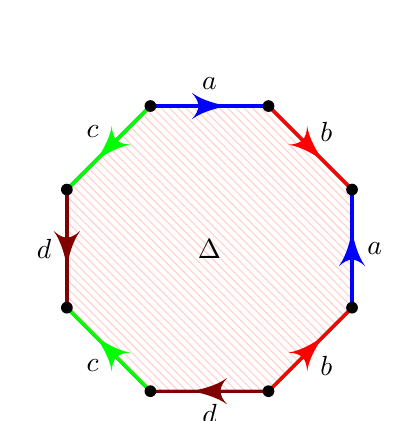
\begin{tikzpicture}

      \def\r{1.960}

      \draw[pattern=north west lines, pattern color=pink, opacity=0.7]
    ({\r*cos(22.5)},   {\r*sin(22.5)}) --
    ({\r*cos(67.5)},   {\r*sin(67.5)}) --
    ({\r*cos(112.5)},  {\r*sin(112.5)}) --
    ({\r*cos(157.5)},  {\r*sin(157.5)}) --
    ({\r*cos(202.5)},  {\r*sin(202.5)}) --
    ({\r*cos(247.5)},  {\r*sin(247.5)}) --
    ({\r*cos(292.5)},  {\r*sin(292.5)}) --
    ({\r*cos(337.5)},  {\r*sin(337.5)}) -- cycle;

      \draw[-<-={1.5},red]
        ({\r*cos(22.5)},  {\r*sin(22.5)})  -- ({\r*cos(67.5)},   {\r*sin(67.5)});
      \draw[-<-={1.5},blue]
        ({\r*cos(67.5)},  {\r*sin(67.5)})  -- ({\r*cos(112.5)},  {\r*sin(112.5)});
      \draw[->-={1.5},green]
        ({\r*cos(112.5)}, {\r*sin(112.5)}) -- ({\r*cos(157.5)},  {\r*sin(157.5)});
      \draw[->-={1.5},mred]
        ({\r*cos(157.5)}, {\r*sin(157.5)}) -- ({\r*cos(202.5)},  {\r*sin(202.5)});
      \draw[-<-={1.5},green]
        ({\r*cos(202.5)}, {\r*sin(202.5)}) -- ({\r*cos(247.5)},  {\r*sin(247.5)});
      \draw[-<-={1.5},mred]
        ({\r*cos(247.5)}, {\r*sin(247.5)}) -- ({\r*cos(292.5)},  {\r*sin(292.5)});
      \draw[->-={1.5},red]
        ({\r*cos(292.5)}, {\r*sin(292.5)}) -- ({\r*cos(337.5)},  {\r*sin(337.5)});
      \draw[->-={1.5},blue] 
        ({\r*cos(337.5)}, {\r*sin(337.5)}) -- ({\r*cos(22.5)},   {\r*sin(22.5)});

      \node[fill, circle, inner sep=1.5pt] at ({\r*cos(22.5)},   {\r*sin(22.5)})   {};
      \node[fill, circle, inner sep=1.5pt] at ({\r*cos(67.5)},   {\r*sin(67.5)})   {};
      \node[fill, circle, inner sep=1.5pt] at ({\r*cos(112.5)},  {\r*sin(112.5)})  {};
      \node[fill, circle, inner sep=1.5pt] at ({\r*cos(157.5)},  {\r*sin(157.5)})  {};
      \node[fill, circle, inner sep=1.5pt] at ({\r*cos(202.5)},  {\r*sin(202.5)})  {};
      \node[fill, circle, inner sep=1.5pt] at ({\r*cos(247.5)},  {\r*sin(247.5)})  {};
      \node[fill, circle, inner sep=1.5pt] at ({\r*cos(292.5)},  {\r*sin(292.5)})  {};
      \node[fill, circle, inner sep=1.5pt] at ({\r*cos(337.5)},  {\r*sin(337.5)})  {};

      \def\R{2.1}
      \node[inner sep=1.5pt, label=center:$a$] at ({\R*cos(0)},     {\R*sin(0)})     {};
      \node[inner sep=1.5pt, label=center:$b$] at ({\R*cos(45)},    {\R*sin(45)})    {};
      \node[inner sep=1.5pt, label=center:$a$] at ({\R*cos(90)},    {\R*sin(90)})    {};
      \node[inner sep=1.5pt, label=center:$c$] at ({\R*cos(135)},   {\R*sin(135)})   {};
      \node[inner sep=1.5pt, label=center:$d$] at ({\R*cos(180)},   {\R*sin(180)})   {};
      \node[inner sep=1.5pt, label=center:$c$] at ({\R*cos(225)},   {\R*sin(225)})   {};
      \node[inner sep=1.5pt, label=center:$d$] at ({\R*cos(270)},   {\R*sin(270)})   {};
      \node[inner sep=1.5pt, label=center:$b$] at ({\R*cos(315)},   {\R*sin(315)})   {};

      \node[inner sep=1.5pt, label=center:$\Delta$] at (0,0) {};

    \end{tikzpicture}
  \end{center}
  The fundamental class $[M] \in H_1(X)$ is
  \[
    a + b - a - b + d + c - d - c
  \]
  We know that
  $H^1(X) = \Z \alpha + \Z \beta + \Z \gamma + \Z \delta$.
  We see that $\alpha_1(a_1) = 1$ %check a_1 in picture
  When we compute $D_M(\alpha_1)$ we get
  \[
    D_M(\alpha_1) = [M] \capp \alpha_1 = -\tau_1 \capp \alpha_1 =
    -\alpha_1(e_1) a_1 - \alpha_1(e_2) b_1 + \alpha_1(e_1) a_1 = -b_1.
  \]
\end{example}

\begin{definition}[Compactly supported cohomology]
  Let $X$ be a locally finite ($\Delta$, CW, or simplicial) complex.
  Then
  \[
    C_C^k :=
    \set{f \in C^k \mid f \text{ is supported on finitely many simplices}}.
  \]
  Check that $\delta \colon C_C^k \to C_C^{k+1}$.
\end{definition}

\begin{remark}
  When $K \subset X$ is compact we denote $K \subset \subset X$.
\end{remark}

\begin{remark}
  In singular cohomology we get that
  \[
    C_C^k(X) = \bigcup_{K \subset \subset X} C^k(X,X-K).
  \]
  or
  \[
    C_C^k(X) = \set{f \colon \text{singular $k$-simplices} \to \Z \mid
    \exists K \st f(\sigma) := f(X - K) = 0}.
  \]
\end{remark}

\begin{remark}
  A partially order set $(X,\le)$ is said to be directed if for
  all $i,j \in I$ there exists $k \in I$ so that $k \geq i,j$.
\end{remark}

\begin{definition}[Direct limit]
  Let $\set{A_i}_{i \in I}$ be a collection is of abelian groups
  so that $(I,\le)$ is a directed partially ordered sets.
  For all $i \le j$ let $f_{ij} \colon A_i \to A_j$ be maps.
  Then
  \begin{align*}
    \varinjlim A_i &=
    \bigoplus A_i /
    \langle \set{a_i - f_{ij}(a_i) \mid i \le j \stand a_i \in A_i} \rangle \\ &=
    \bigsqcup A_i / a_i \sim f_{ij} a_i \quad \forall i \le j \stand a_i \in A_i.
  \end{align*}
\end{definition}

\begin{example}
  The sets $(\N,\le)$
  and $(K,\subseteq)$ where $K$ is the set of all compact subsets of
  a topological space $X$.
\end{example}

\begin{remark}
  We have that $H_C^K(X) = \varinjlim H^k(X,X-K)$
  for $K \subset \subset X$.
\end{remark}

\begin{definition}[Cofinal set]
  We say that $J \subseteq I$ is cofinl if for all $i \in I$
  there exists $j \in J$ such that $i \le j$.
\end{definition}

\begin{definition}[Proper map]
  A map so that the preimage of a compact set is compact is called proper.
\end{definition}

\begin{remark}
  We have that $H_i(X) = \varinjlim_{K \subseteq X} H_i(K)$.
\end{remark}

\begin{remark}
  We have that $D_M \colon \varinjlim_{K} H^i(M \mid K) \to H_{n - i}(M)$.
\end{remark}

\begin{theorem}[Poincar\'e duality]
  Let $M$ be an oriented $n$-manifold with orientation $x \mapsto \mu_x$.
  Then $D_M$ is an isomorphism.
\end{theorem}









\end{document}
